\documentclass{article}
% SI NO PENSAS IMPRIMIRLO EN FORMATO LIBRO PODES USAR
%\documentclass[11pt,a4paper]{tesis}

\usepackage[spanish, es-noshorthands]{babel}
\addto\captionsspanish{\renewcommand{\tablename}{Tabla}} %Para que diga Tabla en vez de Cuadro
\usepackage{dsfont, amsmath, amsthm}

\usepackage{caption}
\usepackage{subcaption}  % Para tener captions dentro de las subfiguras
\captionsetup{font=small}%para que las captions de las figuras sean más chicas

\usepackage{amssymb}
\usepackage{booktabs} % For better table formatting
\usepackage{graphicx} % Required for inserting images
\usepackage[colorlinks=true, urlcolor=blue, linkcolor=blue, citecolor=green]{hyperref}
%linkColor = citas internas cómo ref
\usepackage{tikz}
\usetikzlibrary{arrows.meta}
\usetikzlibrary{decorations.pathmorphing}
\usepackage{algorithm}
\usepackage{algpseudocode}
\usepackage{pgf} % For arithmetic operations in TikZ
\usepackage{comment}
\usepackage{booktabs}
\usepackage{url} %For writing paths
\usepackage[normalem]{ulem}
\usepackage{multirow}
\newcommand{\scc}[1]{{\color{red}#1}}

\usepackage[a4paper,margin=1in]{geometry} %Para achicar los márgenes

% AI stuff
\newcommand{\domain}{\mathds{D}}
\newcommand{\entities}{\texttt{ent}}
\newcommand{\consistsWith}{\texttt{cw}}
\newcommand{\charFunML}{\charactheristicFunction}
\newcommand{\aCircuit}{\mathcal{C}}

% Computational complexity stuff
\newcommand{\NP}{\textsc{NP}}
\newcommand{\NPhard}{\textsc{NP-hard}}
\newcommand{\NPcomplete}{\textsc{NP-complete}}
\newcommand{\sharpPhard}{\textsc{\#P-hard}}

% Sets and probability stuff
\newcommand{\R}{\mathds{R}}
\newcommand{\perm}{perm}
\newcommand{\aDistribution}{\mathcal{D}}
\newcommand{\expectancy}{\mathds{E}}
% Important names and stuff
\newcommand{\SHAPscore}{\textsc{SHAP-score}}
\newcommand{\aBayesianDistribution}{\mathcal{B}}
\newcommand{\set}[1]{ \{ #1 \} }

% Game Theory
\newcommand{\charactheristicFunction}{\nu}
\newcommand{\players}{\mathcal{I}}
\newcommand{\Shap}{Shap}
\newcommand{\assym}{\Shap^{assym}}

% DAG and Assym Notation
\newcommand{\toOr}{\pi} %topologicalOrder
\newcommand{\rel}{R} %relation
\newcommand{\union}{union}
\newcommand{\equivalenceClass}{[\pi]_{\rel}} %equivalenceClass
\newcommand{\eqClassSize}{eqClassTopos}
\newcommand{\equivalenceClassRep}{\mathsf{Rep}(\equivalenceClass)}
\newcommand{\numEqCl}{\#EC} %equivalenceClass formula
\newcommand{\unrEqCl}{UnrEC} %unrelated equivalenceClass formula
\newcommand{\heuristicASVFormula}{\frac{1}{|\topo(G)|} \sum_{\equivalenceClass \in eqCl(G, x_i)} (\charactheristicFunction(\toOr_{<i} \cup \{x_i\}) - \charactheristicFunction(\toOr_{<i})) \cdot |\equivalenceClass|} %New Formula
\newcommand{\eqClassSizes}{eqClassSizes} %unrelated equivalenceClass sizes formula
\newcommand{\leftPossibleOrders}{\#LO} %Left possible orders

%% Drawing graphs

\newcommand{\drawUnrelatedTreeWithColor}[5]{
    \node[circle, draw=#5] (#1) at (#2, #3) {#4};
    \pgfmathsetmacro{\x}{#2-2}
    \pgfmathsetmacro{\y}{#3-0.3} 
    \draw[#5, wiggly] (#2, \y)
        -- ++(-1,-1.6) 
        -- ++(2,0) 
        -- cycle;
    \node[text=#5] at (\x, \y) {#4 subtree};
}

\newcommand{\drawUnrelatedTree}[4]{
    \drawUnrelatedTreeWithColor{#1}{#2}{#3}{#4}{red}
}

\newcommand{\drawUnrelatedTreeWithTag}[6]{
    \drawUnrelatedTreeWithColor{#1}{#2}{#3}{#4}{#5}

    % Texto de nodos disponibles (más abajo del contorno)
    \pgfmathsetmacro{\ysubtree}{#3 - 0.3}
    \pgfmathsetmacro{\ytext}{\ysubtree - 2.0}
    \node[text=#5] at (#2, \ytext) {#6};
}


% Comments and stuff
%\definecolor{darkred}{rgb}{0.55, 0.0, 0.0}
%\usepackage[dvipsnames,svgnames,x11names]{xcolor}
\usepackage[backgroundcolor=orange, textcolor=black, textsize=tiny]{todonotes}
\newcommand{\santi}[1]{\todo[inline,caption={},color=blue!30]{{\bf Santi:} #1}}
\newcommand{\echu}[1]{\todo[inline,caption={},color=orange!30]{{\bf Echu:} #1}}
\newcommand{\sergio}[1]{\todo[inline,caption={},color=green!30, size=\footnotesize]{{\bf Sergio:} #1}} 
\newcommand{\sidesergio}[1]{\todo[caption={},color=green!30, size=\footnotesize]{{\bf Sergio:} #1}}
\newcommand{\aMechanism}[0]{\mathcal{D}}
\newcommand{\anAlgorithm}[0]{\mathcal{A}}

% Graphs and networks
\newcommand{\topo}{topos}
\newcommand{\numTopo}{\#topos}
\newcommand{\aBayesianNetwork}{N}
\newcommand{\parents}{\textit{Parents}}
\newcommand{\dtrees}{\emph{dtrees}}
\newcommand{\dtree}{\emph{dtree}}
\newcommand{\childNetwork}{\emph{Child}}
\newcommand{\cancerNetwork}{\emph{Cancer}}
\newcommand{\variableNetwork}[1]{\texttt{#1}}
\newcommand{\intersectionNode}{i_{\cap}}
\newcommand{\subtree}{s}


% Theorems %Traducidos 18/3
\newtheorem{example}{Ejemplo}
\newtheorem{theorem}{Teorema}
\theoremstyle{plain} %Nota amsthm es necesario para Theoremstyle
% \newtheorem{proposition}[theorem]{Proposition} Si lo hago de este modo todos compartirían el mismo contador y no quiero que eso pase. 
\newtheorem{proposition}{Proposición} 
\newtheorem{lemma}{Lema}
\newtheorem{corollary}{Corolario}
\newtheorem{observation}{Observación}  
\newtheorem{formula}{Fórmula}  
\newtheorem{sketch}{Boceto} 
\newtheorem{acknowledgements}{Agradecimientos}
%
\newtheorem{fact}{Hecho}
%\theoremstyle{definition}  % Para que no sea en italics
%\newtheorem{definition}[theorem]{Definition}

%Definition 

\theoremstyle{definition} % The style more suitable for definitions, examples, etc.
\newtheorem{definition}{Definición}[section] % This will not share the counter with theorems

\tikzset{
    nodo/.style={
        shape=circle,
        draw=black,
        line width=1pt,   
        minimum size=7mm
    },
    arista/.style={
        line width=1pt,  
        -{Latex[length=3mm]}  
    },  
    mySnake/.style={
        decorate, 
        decoration={snake, amplitude=.4mm, segment length=4mm, post length=1mm}
    }
}

\begin{document}



%%%% CARATULA

\def\autor{Ezequiel Companeetz}
\def\tituloTesis{Optimización de ASV para árboles de decisión}
\def\runtitulo{Optimización de ASV para árboles de decisión}
\def\runtitle{ASV optimization for Decision Trees}
\def\director{Santiago Cifuentes}
\def\codirector{Sergio Abriola}
\def\lugar{Buenos Aires, 2025}
\newcommand{\HRule}{\rule{\linewidth}{0.2mm}}
%
\thispagestyle{empty}

\begin{center}\leavevmode

\vspace{-2cm}

\begin{tabular}{l}

\includegraphics[width=2.6cm]{img/logofcen.pdf}
\end{tabular}


{\large \sc Universidad de Buenos Aires

Facultad de Ciencias Exactas y Naturales

Departamento de Computaci\'on}

\vspace{6.0cm}

%\vspace{3.0cm}
%{
%\Large \color{red}
%\begin{tabular}{|p{2cm}cp{2cm}|}
%\hline
%& Pre-Final Version: \today &\\
%\hline
%\end{tabular}
%}
%\vspace{2.5cm}

\begin{huge}
\textbf{\tituloTesis}
\end{huge}

\vspace{2cm}

{\large Tesis de Licenciatura en Ciencias de la Computaci\'on}

\vspace{2cm}

{\Large \autor}

\end{center}

\vfill

{\large

{Director: \director}

\vspace{.2cm}

{Codirector: \codirector}

\vspace{.2cm}

\lugar
}

\newpage\thispagestyle{empty}


%%%% ABSTRACTS, AGRADECIMIENTOS Y DEDICATORIA
\pagestyle{empty}
\section*{\runtitulo}


\noindent En esta tesis se aborda el problema de la explicabilidad en modelos de aprendizaje automático mediante métodos de feature attribution.

En particular, se estudia una variante de los Shapley values conocida como Asymmetric Shapley Values (ASV), que permite incorporar conocimiento causal en la explicación de modelos de forma model-agnostic. A partir del análisis de su complejidad, se demuestra que el cálculo exacto de ASV es polinomial en modelos cuya distribución de entrada está representada por una red bayesiana del tipo Naive Bayes, en contraste con SHAP, que es \#P-hard aún en este caso restringido.

Con el objetivo de extender estos resultados a clases más generales de redes bayesianas, se introduce una noción de clases de equivalencia sobre los órdenes topológicos del grafo causal subyacente, lo cual permite reducir drásticamente el número de permutaciones necesarias para computar ASV. Se presenta un algoritmo polinomial en el número de clases para identificarlas, y se implementa un esquema de cómputo exacto de ASV basado en estas clases. Además, se propone un nuevo método para computar en tiempo polinomial la predicción esperada de un árbol de decisión, sobre una distribución dada por una red bayesiana arbitraria, permitiendo así evaluar el algoritmo desarrollado para el cómputo de ASV en estos modelos. 

Por último, se propone un algoritmo aproximado para calcular el ASV en familias de DAG's causales del tipo polytree. Para ello, se desarrolla un algoritmo de muestreo aleatorio de órdenes topológicos de polytrees. Estos resultados respaldan la viabilidad del enfoque propuesto en estructuras causales realistas, y se contrastan empíricamente con SHAP tanto en precisión como en eficiencia computacional.
    \bigskip
    
    \noindent\textbf{Palabras clave:} Explicabilidad, Árboles de decisión, Asymmetric Shapley Values (ASV), Shap, Polytrees, Ordenes topológicos

\cleardoublepage

\section*{\runtitle}

\noindent This thesis addresses the problem of explainability in machine learning models through feature attribution methods.

In particular, it studies a variant of the Shapley values known as Asymmetric Shapley Values (ASV), which allows for the incorporation of causal knowledge into model-agnostic explanations. Through a complexity analysis, it is shown that the exact computation of ASV is polynomial for models whose input distribution is represented by a Naive Bayes Bayesian network, in contrast to SHAP, which is \#P-hard even in this restricted case.

To extend these results to more general classes of Bayesian networks, a notion of equivalence classes over the topological orderings of the underlying causal graph is introduced. This approach drastically reduces the number of permutations required to compute ASV. A polynomial-time algorithm is presented to identify these classes, and an exact ASV computation scheme based on them is implemented. Additionally, a new method is proposed to compute the expected prediction of a decision tree in polynomial time over a distribution given by an arbitrary Bayesian network, thereby enabling the evaluation of the developed ASV computation algorithm on these models.

Finally, an approximate algorithm is proposed to compute the ASV in families of causal DAGs of the polytree type. To this end, a random sampling algorithm for topological orderings of polytrees is developed. These results support the feasibility of the proposed approach in realistic causal structures and are empirically compared with SHAP in terms of both accuracy and computational efficiency.
\bigskip

\noindent\textbf{Keywords:} Explainability, Decision Trees, Asymmetric Shapley Values (ASV), Shap, Polytrees, Topological Orders


\cleardoublepage
\section*{Agradecimientos}

Primero que nada, agradezco a mis directores, Santiago y Sergio, los cuales no sólo me ayudaron a encontrar un tema acorde a lo que buscaba. Si no que también me dieron excelentes comentarios y correcciones, que me guiaron en el proceso de realizar esta tesis. 

Muchísimas gracias a mi familia, la cual me acompaño en todo este trayecto universitario y sin la cual no hubiera podido llegar adonde estoy. Por la contención, el aguante y por estar ahí.

Muchas gracias a los jurados, Pablo Riera y Eric Brandwein, por tomarse el tiempo de leer y evaluar esta tesis. 

Gracias a Carlos Miguel Soto y Pablo Terlisky por la colaboración con el algoritmo de conteo de órdenes topológicos en polytrees. 

Gracias a mis amigos y compañeros de cursada, los cuales me contagiaron su pasión: Rama, Male, Franquito, Lombi, Chara, Tomi, Pedrito, Fede, Pau, La Plebe, Amigos de Berto y todos los amigos de un cuatri que hice. Realmente no hubiera podido hacerlo sin su apoyo, desde guías resueltas a excelentes compañeros de trabajos prácticos. 

Gracias también a Exactas por ser un espacio tan bello tanto para juntarse a estudiar, jugar al voley o dar clase. 

También estoy muy agradecido de los excelentes docentes del departamento de computación con los que tuve el placer de cursar. Los cuales daban clases que te desafiaban, despertaban tu curiosidad y  lograban transmitirte su pasión. Por último, gracias a la universidad pública por permitir que esto suceda. 
    


 

\cleardoublepage
\tableofcontents

\pagestyle{headings}

%%%% ACA VA EL CONTENIDO DE LA TESIS

\section{Introducción}

\begin{comment}
    Introducción
        XAI y las distintas métricas que existen
            Feature attribution, counterfactual, rule based, sufficient reason, etc
        Algoritmos de feature attribution
        Código fuente 
\end{comment}

Las capacidades de los distintos modelos de inteligencia artificial (IA) han ido creciendo exponencialmente en los últimos años. Tareas que creíamos imposibles de realizar a través de estas técnicas, como la resolución de problemas matemáticos complejos, hoy en día pueden ser resueltas por los LLMs \cite{frontierMath}. No sólo aumentó la complejidad de las tareas que pueden resolver, sino también la complejidad y el tamaño de sus arquitecturas. Los modelos de hace unos años tenían 1e8 parámetros, mientras que hoy en día ya llegan a 1e12. \cite{EpochLargeScaleModels2024}. El problema que esto genera es que cada vez es más difícil entender cómo funcionan y cómo obtienen las respuestas que nos dan. Esto es algo sumamente importante, ya que si uno está utilizando estas técnicas para diagnósticos médicos u otras situaciones igual de delicadas, es fundamental  entender como los modelos alcanzan sus conclusiones . Ahí es donde entra en juego el área de XAI, Explainable Artificial Intelligence.

El objetivo principal de esta área de investigación consiste en encontrar una explicación para las decisiones o predicciones de los distintos modelos de IA, para poder entender el razonamiento detrás de las mismas. Dentro de esta área hay dos ramas principales, la explicabilidad y la interpretabilidad. La primera se centra en obtener estas explicaciones, y es el área en la cual nos centramos en este trabajo. La segunda en entender a los modelos y su representación interna \cite{interpretabilityPaper}. Estas explicaciones no son útiles únicamente en tanto permiten que los usuarios entiendan el porqué de la respuesta, sino también debido a que ayudan a detectar errores o sesgos indeseados que se hayan generado durante el entrenamiento. 

Dentro del área de explicabilidad hay varios tipos de métodos \cite{interpretabilityBook}, los cuales pueden agruparse de acuerdo a distintos ejes:
\begin{itemize}
    \item \textit{Modelo}
        \begin{itemize}
            \item Agnóstico: Son los métodos que se pueden aplicar a todo tipo de modelos. Por ejemplo en SHAP, el método que describiremos más adelante, su valor no depende de la implementación interna del modelo. %\santi{A qué te referís acá?} 
            \item Específico: Son los métodos que tienen una implementación que está acoplada al modelo que buscan explicar, como en el caso de \textit{Tree-Shap} , una versión de SHAP desarrollada para árboles de decisión, que en su implementación utiliza los caminos del árbol para calcular su valor, aprovechando propiedades de la estructura del modelo.
            %\santi{Acá creo que sería mejor usar como ejemplo que en el caso de árboles podés tomar el camino como justificación. Eso es claramente único al modelo, mientras que Tree-shap es un concepto agnóstico al modelo pero que se calcula de forma piola en árboles.} 
        \end{itemize}
    \item \textit{Alcance}
        \begin{itemize}
            \item Explicación global: Busca descubrir cualidades o comportamientos que el modelo tenga en todas sus predicciones. Por ejemplo, para entender por qué un modelo le otorga un préstamo a un individuo, se observa que el nivel de ingresos siempre es un feature relevante. %.\santi{Acá siento que queda medio vago lo de explicar en su totalidad. Una alternativa es "busca descubrir cualidades o comportamientos que el modelo tenga en todas sus predicciones, como por ejemplo si el modelo mira o no la cantidad de metros cuadrados de una casa, pensando en los datasets de Housing".}
            \item Explicación local: Busca descubrir cualidades o comportamiento que el modelo tenga para un conjunto reducido de instancias del dataset. Por ejemplo, para entender por qué un modelo le otorga un préstamo a un individuo, podemos encontrar que para las personas casadas, la cantidad de hijos es un feature que toma más relevancia.  %\santi{Idem anterior, ser mas precisos y ejemplificar.}
        \end{itemize}
    \item \textit{Tipo de explicación:} Hay varias categorías del tipo de explicación que puede tener un método, por ejemplo \textit{feature importance}, el cual asigna valores a cada feature. También hay \textit{interpretaciones visuales} como saliency maps o correlations plots. Incluso hay métodos que generan un modelo más simple a partir del modelo original, como \textit{Lime}. 

    Cabe destacar que no existe un consenso absoluto sobre qué constituye una "explicación" en el contexto de la inteligencia artificial. Muchas de las técnicas mencionadas —como feature attribution o interpretaciones visuales— son aproximaciones pragmáticas a un problema mucho más amplio y complejo, vinculado a cuestiones filosóficas sobre comprensión, causalidad e interpretación humana \cite{MILLER20191, lipton2017mythosmodelinterpretability}. En este sentido, lo que hoy se considera una explicación en XAI responde más a criterios de utilidad y simplicidad interpretativa que a una definición formal y universalmente aceptada.

    %\santi{Ojo que está incompleto. Btw, en esta parte podrías agregar un párrafo cuestionando qué es una explicación, y podemos buscar citas a discusiones más filosóficas. Onda, que quede claro que feature attribution y etc son una aproximación a una ambición filosófica mucho mayor.}\sergio{agreed}
\end{itemize}

En esta tesis nos centramos en \textit{SHAP} \cite{shapOriginalPaper}, el cual es un método que, en principio, provee explicaciones agnósticas al modelo, con un alcance local y que es del tipo de feature attribution. Esto significa que para una predicción individual que realiza el modelo, \textit{SHAP} va a devolver un valor asociado a cada feature de la instancia. Decimos que es agnóstico, puesto que su valor depende simplemente del output del modelo, por lo que no esta acoplado a su representación interna. Aún así, \textit{SHAP} actualmente es un framework que engloba varios tipos de métodos, ya que hay distintas aproximaciones según cuál sea tu tipo de modelo. Por ejemplo, existen métodos como DeepExplainer, TreeExplainer y LinearExplainer dentro del  \textcolor{blue}{\href{https://shap.readthedocs.io/en/latest/index.html}{framework}}  SHAP, los cuales se utilizan para modelos específicos, pero también hay otros métodos como KernelExplainer, que son agnósticos al modelo.

%\santi{Pero no es este el motivo por el cual decimos que es agnóstico, no? Decimos que es agnóstico porque su valor depende únicamente del mappeo de entradas a salidas. O sea, es una propiedad del mappeo subyacente al modelo, ignorando la arquitectura específica. Entiendo que la idea original es esa, y estas versiones que se nombras después son aproximaciones imperfectas (pq muchas veces nisiquiera coinciden con los shapley o SHAP) para modelos particulares.}

Uno de los problemas principales de este framework es lo costoso que es calcularlo, y en particular, hay estudios que analizan esta dificultad desde el punto de vista de la complejidad computacional. Por ejemplo, se demostró que calcular SHAP para un clasificador trivial es NP-completo, o intratable, para datos con distribuciones más o igual de complejas que una Naive Bayes \cite{arenas2021tractability}.
A raíz de esto, nos resultó interesante analizar si existía alguna variación de SHAP, la cual pueda ser calculada en tiempo polinomial para una distribución de red bayesiana. Además, actualmente hay trabajos similares a este, que buscan analizar la complejidad de SHAP según la variante, el modelo y la distribución \cite{marzouk2025computationaltractabilitymanyshapley} %\santi{Hace poco salió este paper, habría que agregarlo en algún lado -> On the Computational Tractability of the (Many) Shapley Values} 

SHAP está basado en los Shapley values \cite{shapley1953value}, un valor de teoría de juegos.  Una variación de los mismos son los assymetric shapley values (ASV), los cuales pueden introducir el factor de causalidad al cálculo de los mismos. De esta manera, se define ASV \cite{frye2019asymmetric}, un framework similar a SHAP, el cual además tiene en cuenta el grafo causal de los datos. El objetivo es esta tesis es lograr calcular ASV en tiempo polinomial de forma exacta y aproximada para datos con distribuciones de redes bayesianas.

\subsection{Explicaciones basadas en causalidad: Un ejemplo comparativo entre SHAP y ASV} \label{asvCaseExample}
%\echu{¿Juega el ejemplo así?}

En esta sección presentamos un ejemplo tomado de la sección 4.1 del artículo original de ASV \cite{frye2019asymmetric}, con el objetivo de ilustrar como la incorporación de información causal puede enriquecer las explicaciones de un modelo. Se utiliza como caso de estudio datos del conjunto Census Income de la UCI \cite{dua2017uci}, en el cual se entrena un modelo (en este caso una red neuronal) para predecir si el ingreso de un individuo supera los \$50\,000. Dado que algunas de las variables demográficas presentes en este conjunto (por ejemplo, la edad) son claramente causas de otras (por ejemplo, el nivel educativo), es especialmente pertinente considerar información causal al interpretar la predicción del modelo. El conjunto $A$ son las variables definidas como los ancestros causales, con $A= \set{age, sex, native \ country, race}$ y el resto de variables son descendientes de estas. Luego en base a estas variables tenemos 

Para este experimento se calculan dos variaciones de SHAP, una \emph{off-manifold} y otra \emph{on-manifold}, la diferencia es la función de probabilidad que ambas usan. En el enfoque \emph{on-manifold} se respetan las restricciones que hay entre las distintas variables, por ejemplo a la hora de calcular SHAP se va a descartar cualquier instancia tal que $age=3 \land occupation = teacher$, ya que eso no es posible. Pero en el enfoque \emph{off-manifold} no va a haber ninguna restricción a la hora de combinar los distintos valores de cada feature. Estas restricciones se obtienen a través de las correlaciones entre las distintas variables del dataset. Además, vamos a calcular los valores globales para SHAP y ASV, esto se realiza haciendo el promedio entre los valores de SHAP y ASV para cada una de las instancias. 
%\santi{Este párrafo queda raro. El lector todavía no sabe que hay una distribución involucrada. Por otro lado, hace unos párrafos dijiste que Shap era local, pero ahora estás asignando scores globales.}

\begin{figure}
    \centering
    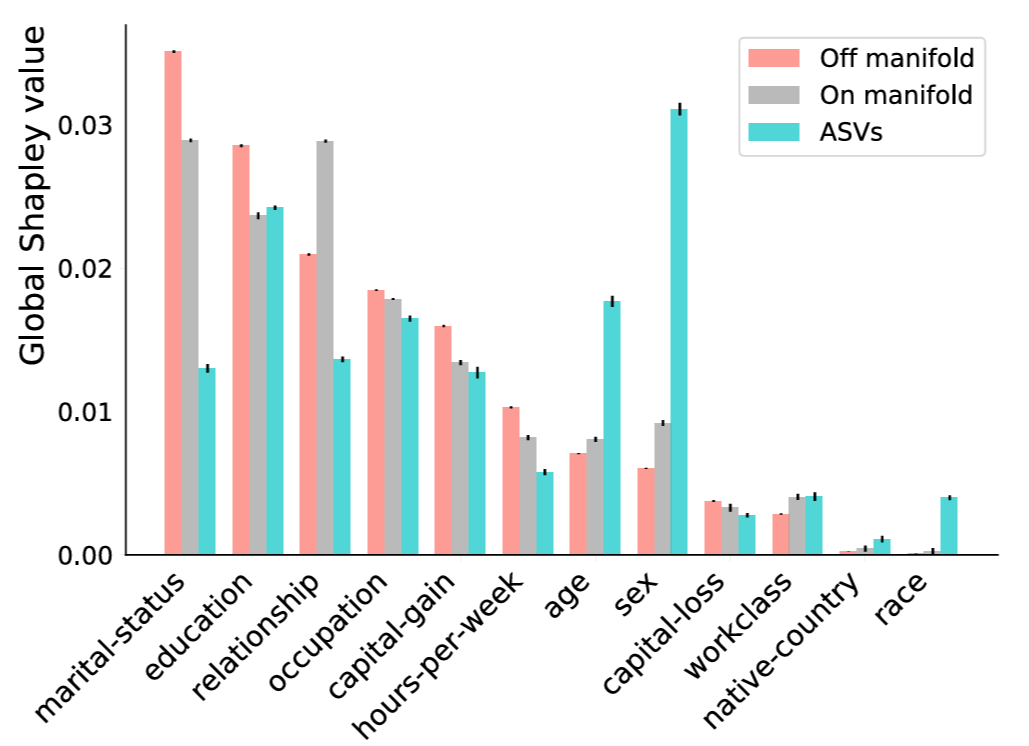
\includegraphics[width=0.5\linewidth]{img/asvPaperPlotExample.png}
    \caption{Valores globales de los Shapley Values y ASV para el modelo entrenado para el Census Income dataset.}
    \label{fig:asvPaperPlotExample}
\end{figure}

La Figura \ref{fig:asvPaperPlotExample} muestra como la variable \emph{género} presenta un Shapley value relativamente pequeño en el análisis off-manifold. En cambio, al incorporar el conocimiento causal mediante ASV, se observa que dicha variable recibe un valor significativamente mayor. Este hallazgo evidencia que, a pesar de que el género tenga una influencia moderada en el modelo cuando se considera de forma aislada, su papel en la explicación se amplifica una vez que se tiene en cuenta su relación causal con otras variables (como el estado civil o la relación actual). De esta forma, los ASVs proporcionan una medida más precisa y contrastada de la contribución de cada variable, permitiendo detectar aspectos de discriminación o sesgo que de otro modo pasarían desapercibidos.

Este ejemplo evidencia cuándo es útil incorporar información causal en la explicación de modelos: en situaciones donde se conoce una relación de causa y efecto entre las variables, el uso de ASVs no solo mejora la interpretabilidad de la explicación, sino que también aporta una perspectiva más fiel al proceso generador de los datos, contribuyendo así a la construcción de modelos más transparentes y confiables.

%\sergio{En general me parece que hay que poner más motivación y ejemplos en esta sección. Estos también pueden servir para ser referenciados y hacer más concretos los conceptos que se introducen después, como ser en la sección 2.}

%\santi{Agreed. Haría un ejemplito con una predicción, y un típico gráfico de esos que muestran los SHAP scores. Idealmente es un ejemplo donde por no tener cuenta correlaciones se asignan mal los scores. Dps cuando introducis ASV mostras que usando la red causal mejora el ranking (i.e. refleja mejor la importancia de los features)}


\subsection{Código fuente}

Todos los algoritmos presentados en este trabajo fueron implementados. El código fuente puede ser encontrado online en el siguiente repositorio: 

\begin{table}[H]
\centering
\begin{tabular}{ll}
\toprule
\textbf{Repository} & \textbf{Repository} \\
\midrule
Source code & \url{https://github.com/EchuCompa/pasantia-BICC} \\
\end{tabular}
\end{table}

\section{Introducción a Shapley y ASV}\label{Section:ComplejidadShap}

\begin{frame}{Definiciones}
	\dificultyLevel{2}
	\begin{itemize}
		\item Sean $X$ los features y $ent(x)$ el conjunto de entidades.
		\item Luego $M$ es el modelo y $\phi$ un \textit{feature attribution score}
	\end{itemize}
	\begin{figure}
		\centering
		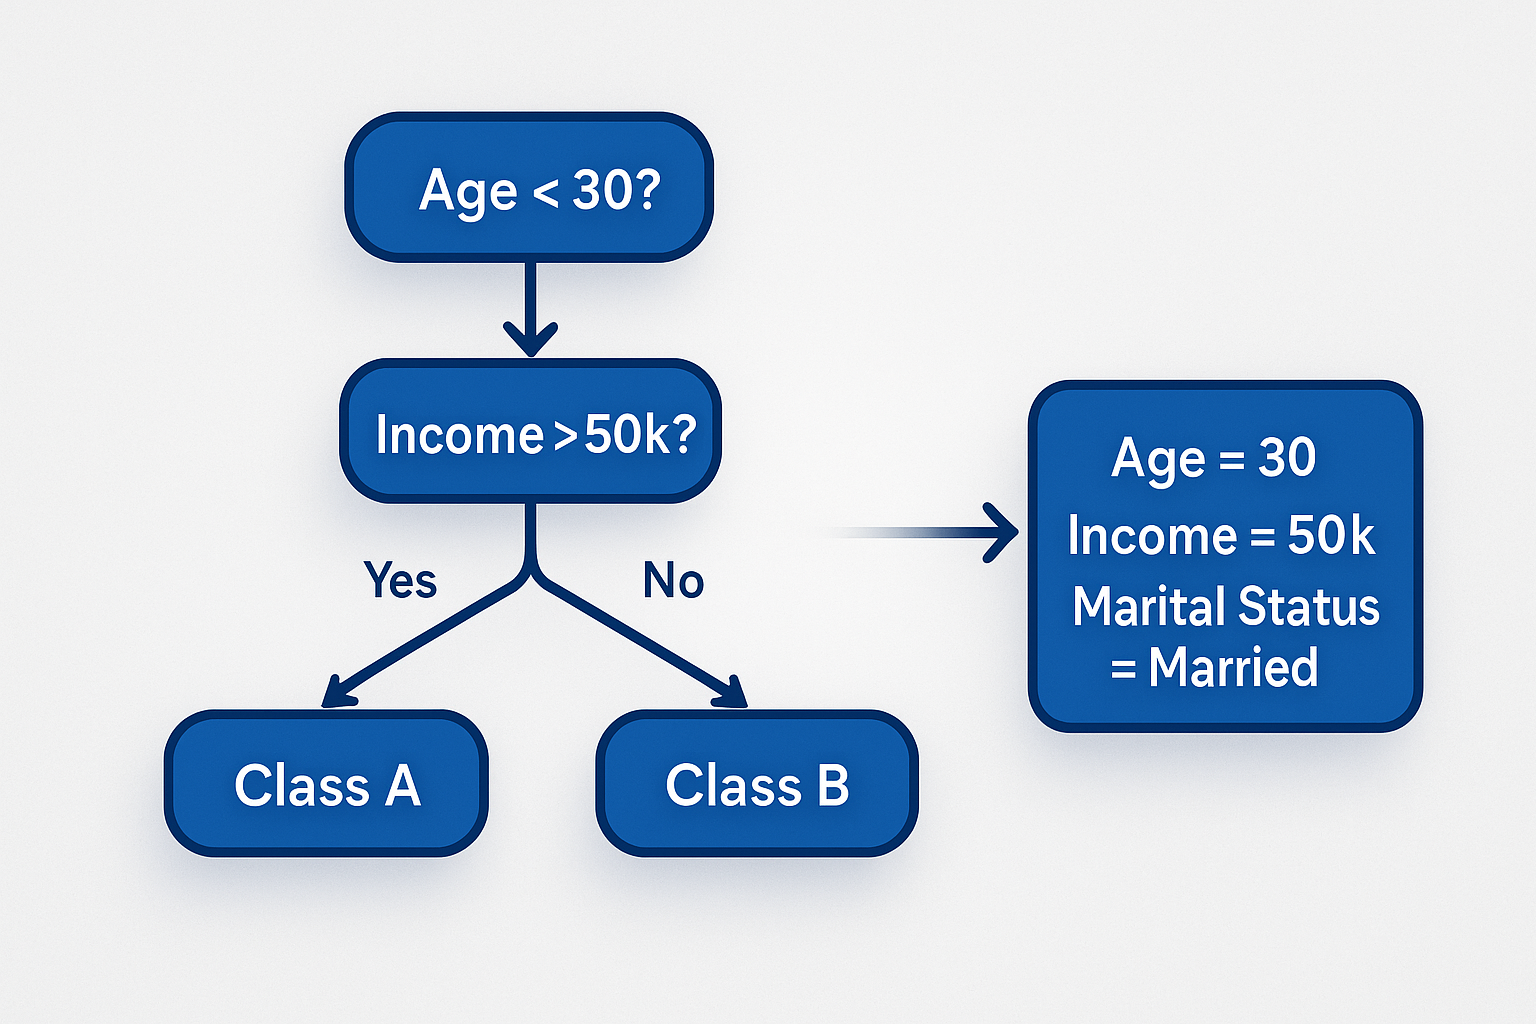
\includegraphics[width=0.7\linewidth]{pic/img/XAI/modelAndEntityExample.png}
	\end{figure}
\end{frame}


\begin{comment}
	\begin{frame}{Definiciones}
		\dificultyLevel{2}
		\begin{mydefinition}[Entidades]
			Sea $X$ el conjunto de features, definimos a $ent(X)$ cómo el conjunto de todas las entidades, con un espacio de probabilidad definido por una distribución $Pr$.
		\end{mydefinition}
	\end{frame}
	
	\begin{frame}{Definiciones}
		\begin{mydefinition}[Modelo]
			Un modelo $M$ es una función  $\phi : ent(X) \to \set{0,1}$, que dada una entidad $e$ devuelve 0 o 1, siendo esta su clasificación.
		\end{mydefinition}
		\begin{mydefinition}[Feature attribution score]
			Un \textit{feature attribution score} es una función $\phi : X \to \mathbb{R}$, esta indica la \textit{relevancia} de cada feature con respecto a una predicción $M(e)$.
		\end{mydefinition}
	\end{frame}
\end{comment}

\begin{frame}{Shapley Values}
    \dificultyLevel{2}
    \textbf{SHAP} se basa en los \textit{Shapley Values} de teoría de juegos cooperativos. Podemos interpretar a este valor $\phi_i(\charactheristicFunction)$ como el aporte del jugador $i$ al juego definido por la función $\charactheristicFunction$.
\end{frame}

\begin{frame}{Asado Familiar : Subconjunto original}
		\begin{figure}
		\centering
		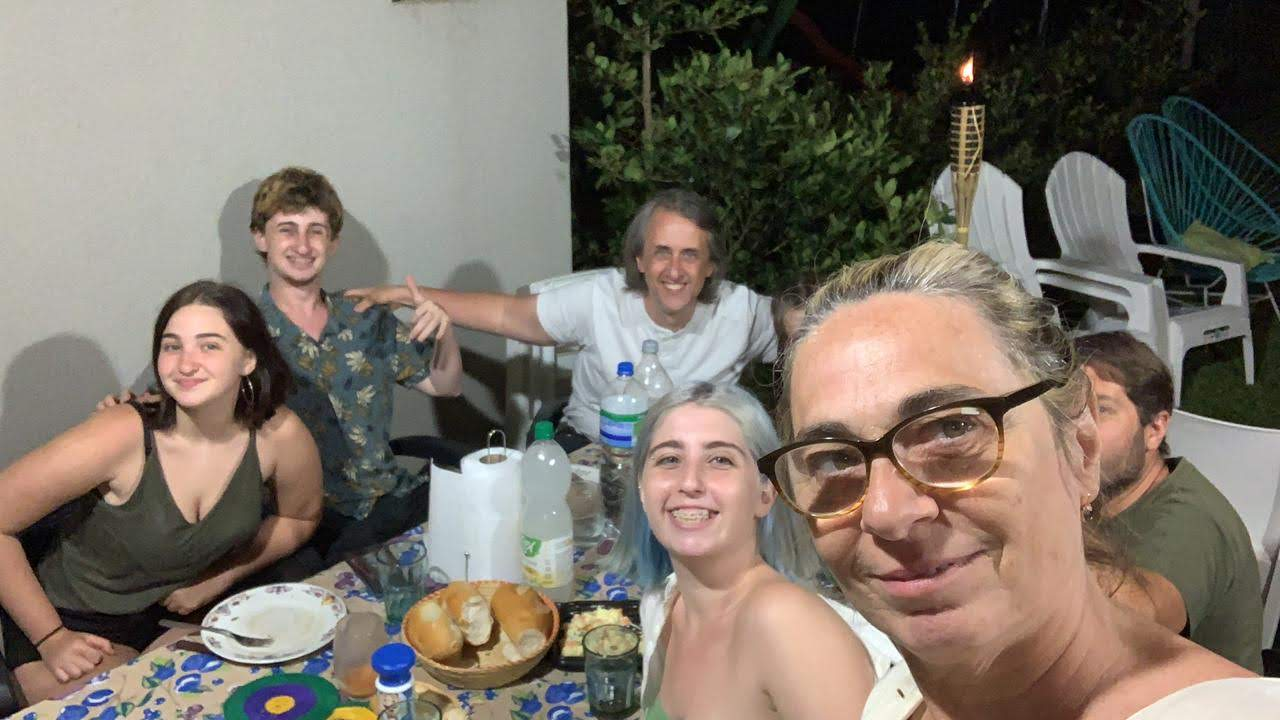
\includegraphics[width=0.9\linewidth]{pic/img/XAI/subconjuntoTotal.jpg}
	\end{figure}
\end{frame}

\begin{frame}{Asado Familiar : Subconjunto óptimo}
	\begin{figure}
		\centering
		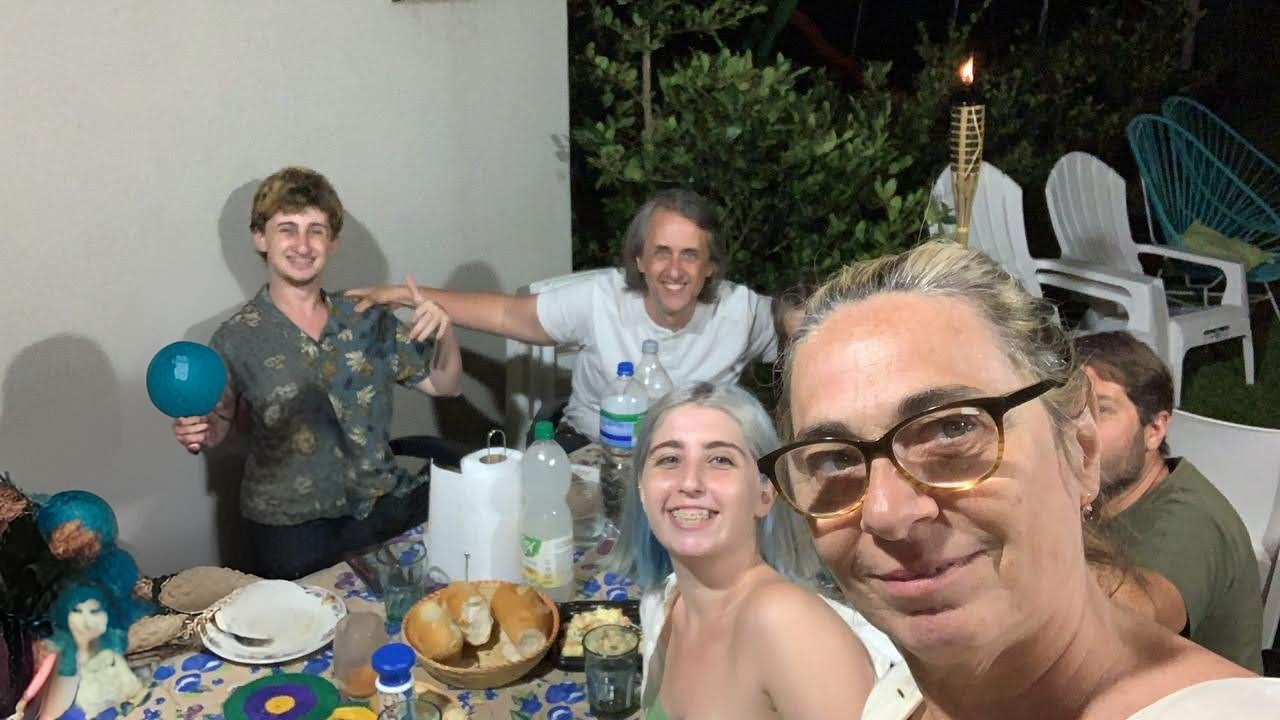
\includegraphics[width=0.9\linewidth]{pic/img/XAI/subconjuntoOptimo.png}
	\end{figure}
\end{frame}

\begin{comment}
	Definición Shapley Values: Ejemplo
	El "Juego": Medir el nivel de éxito y disfrute de un asado familiar, en una escala del 1 (intoxicación masiva) al 10 (gloria culinaria). La "predicción base" o el resultado promedio de cualquier juntada es un 6.
	Los "Jugadores" (Features):
	El que pone la casa y la parrilla.
	El que trae una ensalada de rúcula y parmesano espectacular.
	La que compra un vino de calidad cuestionable.
	Tu hermana (jugador i), que no trajo nada, usó tu silla preferida y se quejó del punto de la carne.
	
\end{comment}

\begin{frame}{Propiedades Shapley Values}
	Las propiedades de los \textit{Shapley Values} son:
	\begin{itemize}
		\item \textbf{Eficiencia:} Toda la ganancia es distribuida 
		%La sumatoria de los shapley values para cada feature es igual a la predicción promedio del modelo. 
		\item \textbf{Simetría:} Jugadores equivalentes reciben el mismo valor.  
		%Si para todas las coaliciones a las que se suman estos jugadores, su valor es el mismo -> tienen el mismo shapley value
		\item \textbf{Linealidad:} El valor de Shapley es lineal respecto a la función característica. 
		% Podes sumar y multiplicar las funciones características, y los shapley values se verán linealmente afectados.  -> \phi_i(a \v + \v2) =  a \phi_i(\v) + \phi_i(\v2)
		\item \textbf{Jugador Nulo:} Si no aporta, su valor es 0.
	\end{itemize}
\end{frame}

\begin{frame}{Fórmula Shapley}
	\dificultyLevel{3}
	\textbf{Fórmula general:}
	
	% Parte visual progresiva de la fórmula
	\only<1,2>{%
		\begin{mydefinition}[Shapley Value]
			\[
			\phi_i(\charactheristicFunction) = \text{Shapley Value del jugador $i$ para la función $\charactheristicFunction$}
			\]
		\end{mydefinition}
	}
	\only<3>{%
		\begin{mydefinition}[Shapley Value]
			\[
			\phi_i(\charactheristicFunction) = \alert<3>{\charactheristicFunction(\pi_{<i}\cup\{i\}) - \charactheristicFunction(\pi_{<i})}
			\]
		\end{mydefinition}
	}
	\only<4>{%
		\begin{mydefinition}[Shapley Value]
			\[
			\phi_i(\charactheristicFunction) = \alert<4>{\sum_{\pi \in perm(X)}}\; \charactheristicFunction(\pi_{<i}\cup\{i\}) - \charactheristicFunction(\pi_{<i})
			\]
		\end{mydefinition}
	}
	\only<5>{%
		\begin{mydefinition}[Shapley Value]
			\[
			\phi_i(\charactheristicFunction) = \alert<5>{\frac{1}{|X|!}}\; \sum_{\pi \in perm(X)} \bigl(\charactheristicFunction(\pi_{<i}\cup\{i\}) - \charactheristicFunction(\pi_{<i})\bigr)
			\]
		\end{mydefinition}
	}
	
	\only<2>{
		\begin{mydefinition}
			La función característica se define como:
			\[
			\charactheristicFunction : \mathcal{P}(X) \to \mathbb{R}
			\]
			Asigna un real a cada posible \textit{coalición} de jugadores, es decir, a cada subconjunto de \( X \).
		\end{mydefinition}
	}
	
	% Lista explicativa
	\begin{itemize}
		\item<3-> \alert<3>{Se calcula cuánto colabora $i$ a $\pi$: $\charactheristicFunction(\pi_{<i}\cup\{i\})-\charactheristicFunction(\pi_{<i})$.}
		\item<4-> \alert<4>{Se suman todas las permutaciones de $X$, para ver cuánto colabora $i$ a cada una.}
		\item<5-> \alert<5>{Se divide todo por $|X|!$, porque se está promediando sobre todas las permutaciones posibles.}
	\end{itemize}
\end{frame}


\begin{comment}

	\begin{frame}{Fórmula función característica en ML}
		\dificultyLevel{3}
		% Parte visual progresiva de la fórmula
		\only<1>{%
			\begin{mydefinition}[Función característica]
				\scriptsize
				\[
				v_{M,e,\Pr}(S) = \text{Predicción promedio de $M$ cuando los features $S$ toman los valores de $e$}
				\]
			\end{mydefinition}
		}
		\only<2>{%
			\begin{mydefinition}[Función característica]
				\[
				v_{M,e,\Pr}(S) = \alert<2>{\sum_{e' \in \consistsWith(e,S)}} \cdots
				\]
			\end{mydefinition}
		}
		\only<3>{%
			\begin{mydefinition}[Función característica]
				\[
				v_{M,e,\Pr}(S) = \sum_{e' \in \consistsWith(e,S)} \alert<3>{\Pr[e'|\consistsWith(e,S)]} \cdot \cdots
				\]
			\end{mydefinition}
		}
		\only<4,5>{%
			\begin{mydefinition}[Función característica]
				\[
				v_{M,e,\Pr}(S) = \sum_{e' \in \consistsWith(e,S)} \Pr[e'|\consistsWith(e,S)] \cdot \alert<4>{M(e')}
				\]
			\end{mydefinition}
		}
		
		% Lista explicativa
		\begin{itemize}
			\item<2-> \alert<2>{Se consideran las instancias $e'$ que coinciden con la entidad $e$ en los atributos de $S$: $\consistsWith(e,S)$.}
			\item<3-> \alert<3>{Se pondera cada $e'$ según su probabilidad condicional dado que coincide con $e$ en $S$: $\Pr[e'|\consistsWith(e,S)]$.}
			\item<4-> \alert<4>{Se evalúa el modelo $M$ sobre cada $e'$.}
			\item<5-> \alert<5>{En resumen: $v(S)$ es la predicción promedio del modelo dejando fijos los features de $S$.}
		\end{itemize}
	\end{frame}
\end{comment}



\begin{frame}{SHAP en Aprendizaje Automático}
\dificultyLevel{2}
	\begin{itemize}
	    \item Features $X$ son los jugadores, y $\charactheristicFunction_{M,e,Pr}(S)$ es la predicción promedio.
	    %\item Utilizamos la fórmula $c_m$ para agrupar permutaciones con el mismo subconjunto. 
	    \item Así la fórmula de SHAP nos queda: \pause
	    %\item Por último utilizando la notación $c_m = \frac{m! (|X|-m-1!)}{|X|!}$, podemos encontrar la fórmula de Shap. \pause 
	    \begin{mydefinition}[SHAP]
	    Teniendo un modelo $M$, una entidad $e$, un feature $x_i$ y una función de probabilidad $Pr$ definimos $\Shap$ como:
	    \[ \Shap_{M,e,\Pr}(x_i) = \sum_{S \subseteq X \setminus \{x_i\}} c_{|S|} (\charactheristicFunction(S \cup \{x_i\}) - \charactheristicFunction(S)) \]    
	    \end{mydefinition}
	    %Mencionar las críticas a SHAP cómo:
	        %Nótese que los axiomas que estos valores satisfacen no tienen un significado claro en el contexto de la inteligencia artificial, ya que dependen de la definición de v[10]. Además, para algunas nociones simples y robustas de atribución de características basadas en explicaciones abductivas [22], los valores de Shapley no logran asignar un puntaje de 0 a features irrelevantes [11].
	    
	\end{itemize}
\end{frame}

% Slide 1: Motivación y definición general
\begin{frame}{Asymmetric Shapley Values (ASV)}
\dificultyLevel{2}

\begin{itemize}[<+- | alert@+>]
	\item La definición clásica de Shapley values asigna el \textbf{mismo peso a todas las permutaciones}.
	\item En ASV se busca \textbf{asignarle más peso a ciertas permutaciones}.  
	\item Para capturar esta idea \textbf{relajamos la propiedad de la simetría}, definiendo una función de peso $w$ sobre las permutaciones
	%\[	w : \perm(\players) \to \R 	\quad\text{con}\quad 	\sum_{\pi} w(\pi)=1\,, 	\]
\end{itemize}
%Sin embargo, cuando hay relaciones causales entre features, algunos órdenes no son coherentes (p.ej. evaluar “educación” antes que “edad”).  


\end{frame}

\begin{frame}{Definición formal de ASV}
\dificultyLevel{3}

\begin{mydefinition}[Asymmetric Shapley Values]
Dada una función característica
\(\;\charactheristicFunction : \mathcal{P}(\players)\to\R\)\; y un peso \(w\) sobre permutaciones, los ASV son
\[
\phi^{assym}_i(v)
\;=\;
\sum_{\pi \in \perm(\players)} 
   \alert{w(\pi)}\bigl(\charactheristicFunction(\pi_{<i}\cup\{i\})-\charactheristicFunction(\pi_{<i})\bigr).
\]
\end{mydefinition}

\end{frame}

\begin{frame}{Ejemplo : Naive Bayes como DAG causal}
\dificultyLevel{2}
    \begin{figure}[ht]
    \centering
    \scalebox{0.8}{
        \begin{tikzpicture}[
            every node/.style={circle, minimum size=1.2cm, font=\small, text=white},
            class/.style={draw, fill=red!70},
            feature/.style={draw, fill=blue!60},
            node distance=1.8cm and 1.8cm,
            ->, thick
        ]
    
            % Central class node
            \node[class] (Disease) {Enfermo};
    
            % Features aligned horizontally below
            \node[feature, below left=of Disease, xshift=-3.6cm] (Fever) {Fiebre};
            \node[feature, right=of Fever] (Cough) {Tos};
            \node[feature, right=of Cough] (Fatigue) {Fatiga};
            \node[feature, right=of Fatigue] (Test) {Dolor};
            \node[feature, right=of Test] (Age) {Edad};
    
            % Edges
            \draw (Disease) -- (Fever);
            \draw (Disease) -- (Cough);
            \draw (Disease) -- (Fatigue);
            \draw (Disease) -- (Test);
            \draw (Disease) -- (Age);
    
        \end{tikzpicture}
    }
	\end{figure}
    
   % \pause     
    %\begin{itemize}     	\item En el caso que nuestro DAG $G$ fuera esta red de ejemplo, las únicas permutaciones válidas serían las cuáles contengan al nodo \textbf{Enfermo} primero.     \end{itemize}
\end{frame}


\begin{frame}{Función de peso desde un DAG causal}
	\dificultyLevel{2}
	
	Dado un DAG causal \(G=(X,E)\). El conjunto de \textbf{órdenes topológicos} son las permutaciones que respetan al grafo causal. % \(\topo(G)\subseteq\perm(X)\).
	\begin{figure}
		\centering
		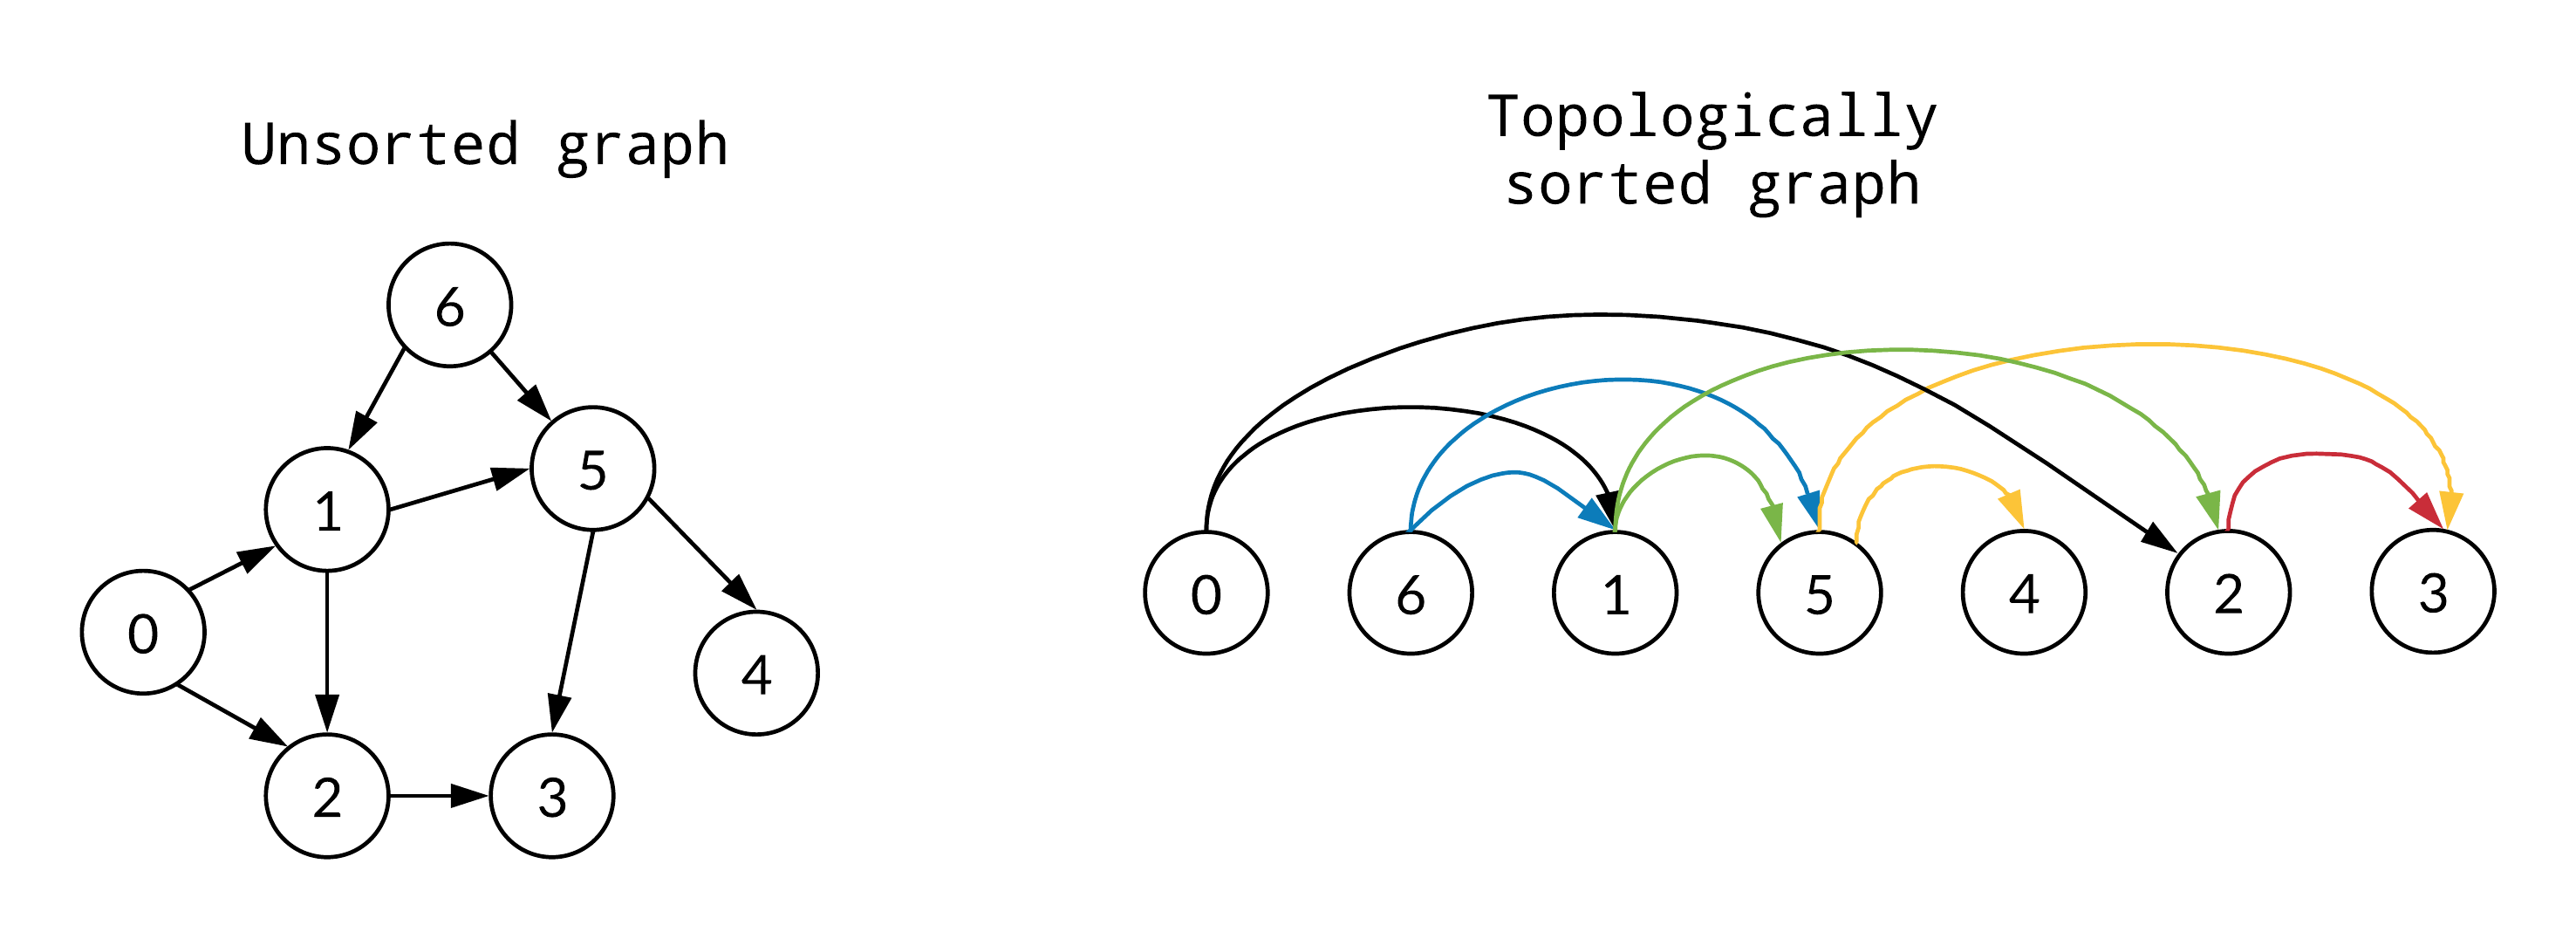
\includegraphics[width=0.9\linewidth]{pic/img/SHAP/topologicalSortExample.png}
	\end{figure}
\end{frame} 

\begin{comment}
		\only<2>{
		\begin{mydefinition}[Orden topológico]
			Dado un grafo dirigido acíclico (DAG) \(G = (V, E)\), un orden topológico es una permutación \(\pi\) de los nodos \(V\) tal que para toda arista \((u, v) \in E\), se cumple que \(\pi(u) < \pi(v)\).
			
			Esto garantiza que todo nodo aparece después de sus predecesores en el grafo.
		\end{mydefinition}
	}
\end{comment}

\begin{frame}{Función de peso desde un DAG causal}
	\dificultyLevel{3}
	
	Así es como \textbf{cada orden recibe el mismo peso}, y cada permutación que \textbf{no es un orden tópologico no debe ser contabilizada}. De esta forma $w$ nos queda:
	\[
	w(\pi)=
	\begin{cases}
		\displaystyle \tfrac1{|\topo(G)|},&\pi\in\topo(G),\\
		0,&\text{en otro caso.}
	\end{cases}
	\]
	
\end{frame}


\begin{frame}{ASV en aprendizaje automático}
	\dificultyLevel{3}
	
	\begin{mydefinition}[ASV con DAG Causal]
		%Teniendo un modelo \(M\), una entidad \(e\), un feature \(x_i\), una función de probabilidad \(\Pr\), y un DAG causal \(G\) sobre los features, definimos \(\assym\) como: \pause
		\[
		\assym_{M,e,\Pr}(x_i) = \alert{\frac{1}{|\topo(G)|}} \sum_{\alert{\pi \in \topo(G)}} \left( \charactheristicFunction(\pi_{<i} \cup \{x_i\}) - \charactheristicFunction(\pi_{<i}) \right)
		\]
	\end{mydefinition}
	\pause
	\begin{itemize}[<+- | alert@+>]
		\item Es la misma fórmula que SHAP, solo que tomamos las permutaciones que sean órdenes topológicos
		\item Este enfoque prioriza las permutaciones causalmente válidas y \textit{asigna más importancia} a las causas que a las consecuencias.
	\end{itemize}
	
\end{frame}

%TODO: Meter meme de basta de fórmulas o algo por el estilo

\begin{comment}
	\begin{frame}{Complejidad Computacional de SHAP y ASV}
		\dificultyLevel{3}
		En ~\cite{van2022tractability} Guy Van et al. demostraron que:
		\begin{itemize}[<+- | alert@+>]
			\item El cálculo general de SHAP es $\sharpPhard$.
			\item Con la distribución \textit{empírica}, SHAP es $\sharpPhard$ incluso para árboles.
			\item Con la distribución Naive Bayes con modelo trivial $f(x)=x_1$, también es $\sharpPhard$.
			\item SHAP es tratable para una familia de modelos bajo distribución \textit{producto} sii el promedio es tratable
		\end{itemize}
		
	\end{frame}
\end{comment}

\begin{comment}
	\item Formalmente, si \(X = \{x_1, \ldots, x_n\}\), con raíz \(x_1\), entonces:
	\[
	\Pr[e] = \Pr[x_1 = e(x_1)] \cdot \prod_{j=2}^{n} \Pr[x_j = e(x_j) \mid x_1 = e(x_1)]
	\]
\end{comment}

\begin{comment}
	\begin{frame}{Ejemplo: Distribución Naive Bayes}
		\dificultyLevel{2}
		
		\begin{itemize}
			\item Una red Naive Bayes define una \textbf{distribución de probabilidad sobre entidades } \(e\), basada en un nodo raíz que condiciona a todos los demás. \pause
			
			\item En nuestro contexto, usamos esta \textbf{distribución como la \(\Pr\) y $DAG$ causal} de nuestras entidades. Podría ocurrir que el grafo causal sea distinto a esta red. 
		\end{itemize}
		
		\begin{figure}[ht]
			\centering
			\scalebox{0.6}{
				\begin{tikzpicture}[
					every node/.style={circle, minimum size=1.2cm, font=\small, text=white},
					class/.style={draw, fill=red!70},
					feature/.style={draw, fill=blue!60},
					node distance=1.8cm and 1.8cm,
					->, thick
					]
					% Central class node
					\node[class] (Disease) {Enfermo};
					
					% Features aligned horizontally below
					\node[feature, below left=of Disease, xshift=-3.6cm] (Fever) {Fiebre};
					\node[feature, right=of Fever] (Cough) {Tos};
					\node[feature, right=of Cough] (Fatigue) {Fatiga};
					\node[feature, right=of Fatigue] (Test) {Dolor};
					\node[feature, right=of Test] (Age) {Edad};
					
					% Edges
					\draw (Disease) -- (Fever);
					\draw (Disease) -- (Cough);
					\draw (Disease) -- (Fatigue);
					\draw (Disease) -- (Test);
					\draw (Disease) -- (Age);
				\end{tikzpicture}
			}
		\end{figure}
	\end{frame}
\end{comment}


\begin{frame}{Complejidad de ASV}
	\dificultyLevel{2}
	Nuestro objetivo es estudiar la \textbf{tratabilidad} de ASV para los casos que SHAP no es tratable.Luego teniendo en cuenta que: \pause 
	
	\begin{itemize}[<+- | alert@+>]
		\item El conjunto sobre el cual se itera en ASV es más reducido que el de SHAP
		\item La distribución Naive Bayes se asemeja a una producto.
	\end{itemize}
	
	\pause
	llegamos a nuestro primer resultado: 
	\begin{mytheorem}[Tratabilidad de ASV]
		\small
		ASV puede calcularse en tiempo polinomial bajo una distribución Naive Bayes para una familia de modelos $\mathcal{F}$ si y solo si SHAP puede calcularse para $\mathcal{F}$ bajo distribución producto.
	\end{mytheorem}
\end{frame}

\begin{frame}{Objetivo de la tesis}
	\dificultyLevel{2}
	\begin{itemize}[<+- | alert@+>]
		\item A raíz del teorema anterior surge el objetivo inicial de la tesis, el cuál era realizar \emph{el cálculo exacto de ASV en tiempo polinomial para una red bayesiana.} 
		\item Como vamos a necesitar evaluar a $\charactheristicFunction$, necesitamos un modelo el cual pueda calcular el promedio en tiempo polinomial. Por eso nos vamos a centrar en \textbf{árboles de decisión.}
		\item El cálculo del promedio va a depender de su distribución $Pr$, que en este caso es una \textbf{Red Bayesiana}. 
		%\item Por lo que es necesario entender estas distribuciones para poder realizar este cálculo. 
	\end{itemize}
	
\end{frame}

\newpage

\section{Grafos Causales}\label{Section:RedesBayesianas}

%\santi{Para mi esto debería estar antes. Principalmente porque ya aparecio una red bayesiana en la demo anterior. Capaz podes ponerlo pegado a la seccion 3.1, que es también medio introductoria. Sino también puede ir antes}

\begin{comment}
    Una Red Bayesiana para features \(X\) es una tupla \(\aBayesianNetwork = (X, E, \Pr)\), donde \((X, E)\) es un DAG que tiene los features \(X\) como nodos, $E$ sus aristas y \(\Pr\) es una función que codifica, para cada feature \(X\), su distribución de probabilidad condicional \(\Pr(X | \parents(X))\). La semántica topológica especifica que cada variable es condicionalmente independiente de sus no-descendientes, dado sus padres (y es por esto que la información de \(\Pr\) es suficiente para reconstruir la distribución conjunta de \(X\)).

\echu{¿Tiene sentido poner esta definición acá si después vamos a definirlo de vuelta en la siguiente sección? Podemos poner sólo la de la naive bayes sin tener en cuenta la de la red bayesiana. }
\sergio{Creo que es mejor evitar repetición directa, y además es mejor si se introducen los nuevos conceptos de manera más gradual cuando tiene sentido}
\santi{Banco a muerte no repetir, pero soy de la escuela de definir todo al principio. Da igual de todas formas.}

Dada una Red Bayesiana \(\aBayesianNetwork\), sea \(\pi \in perm(X)\) un orden topológico para el DAG de \(\aBayesianNetwork\). Entonces, la probabilidad para alguna entidad \(e\) se calcula como \footnote{A partir de ahora, denotamos por \(X_i\) la variable aleatoria asociada al feature \(x_i\).}

\begin{align}\label{eq:bayesian_probability}
    \Pr[e] = \Pr\left[\bigwedge_{i=1}^n X_i = e(x_i)\right] &= \prod_{i=1}^n \Pr\left[X_{\pi(i)} = e(x_{\pi(i)}) | \bigwedge_{i=1}^{i-1} X_{\pi(i)} = e(x_{\pi(i)})\right]\nonumber \\
    &= \prod_{i=1}^n \Pr\left[X_{\pi(i)} = e(x_{\pi(i)}) | \bigwedge_{x_j \in \parents(x_i)} X_j = e(x_j)\right]
\end{align}

donde en la última desigualdad usamos las restricciones topológicas para condicionar únicamente en los padres de \(x_i\). \cite{Darwiche_2009} Esta fórmula se basa en utilizar el teorema de Bayes para descomponer a la conjunción de valores que representa la entidad $e$ en varias probabilidades condicionales utilizando las distintas dependencias entre las variables que tiene un orden tópologico. 

Este modelo se basa en un grafo acíclico dirigido (DAG) donde la variable objetivo \(Y\) es el único nodo padre y todos los features \(X_i\) son hijos independientes. Dado que cualquier familia razonable de modelos contiene este tipo de funciones, la posibilidad de desarrollar algoritmos eficientes para calcular los Shapley values bajo distribuciones bayesianas parece limitada. Aún así hay familias de modelos para los cuáles se puede computar si tenemos una distribución de Markov \cite{marzouk2024tractabilityshapexplanationsmarkovian}.

%\echu{¿Meto esto que esta en el comment en algún lado o ya lo elimino? No se si suma tanto } Rta Cifu: No suma tanto, afueraa esto

\end{comment}

Como mencionamos en la sección anterior, $ASV$ utiliza el grafo causal asociado al problema para definir una función $w$, que nos va a permitir filtrar permutaciones no deseadas que no respeten la causalidad. Luego cuando tenemos una permutación $\topo$ que sí nos interesa, vamos a querer realizar la operación $\charactheristicFunction(\pi_{<i})$, la cual consiste en evaluar la esperanza teniendo en cuenta nuestra distribución elegida y un valor fijo para los feature en $\pi_{<i}$. Para realizar este cálculo necesitamos entender cómo se calculan probabilidades en una red bayesiana y cuál es su complejidad. 

\subsection{Redes Bayesianas}
Una Red Bayesiana $\aBayesianNetwork$ es un $DAG$, donde cada nodo representa una variable diferente y los arcos representan las dependencias condicionales entre ellas, puesto que para calcular la probabilidad de la cabeza necesitamos la de la cola. Por ejemplo, si tenemos el arco $A \longrightarrow B$, esto representa que la variable $B$ depende\footnote{Aunque no necesariamente significa que $A$ dependa de $B$ causalmente, puesto que podríamos armar una red bayesiana que no se condiga con el DAG causal de las variables. } de $A$, y esto se cuantifica usando la probabilidad condicional $P(B|A)$. Un nodo puede tener múltiples padres, por lo que la distribución de los valores del nodo se definirá en una \emph{Tabla de Probabilidad Condicional} (CPT), que define la probabilidad de que tome algún valor, dado los posibles valores de sus nodos padres. Con esto, podemos definir una Red Bayesiana como:

%\santi{Diría que esto es \textit{Intuitivamente}. Nada impide que armes una red bayesiana con todas las dependencias al revés. El truco es que si respetas la causalidad la red debería quedar con pocos ejes, pero en principio cualquier distribución se puede representar tomando cualquier ordenamiento de las variables aleatorias. La definción correcta correcta es que tenés tablitas, y se definen en función de los padres, y todas las tablas juntas dan una distribución.} Echu : Con dependencias condicionales me refería a que dependen en la probabilidad condicional de sus padres
% \santi{Creo que esto queda mejor en un footnote.}

\begin{definition}
Una Red Bayesiana para variables \(X\) es una tupla \(\aBayesianNetwork = (X, E, \Pr)\), donde \((X, E)\) es un DAG que tiene las variables \(X\) como nodos, $E$ como aristas y \(\Pr\) es una función que codifica, para cada variable \(x \in X\), su distribución de probabilidad condicional \(\Pr(x | \parents(X))\):

\begin{itemize}
    \item Para cada variable $x \in X$, sabemos que $x$ tiene un conjunto finito de estados mutuamente excluyentes, estos son los posibles valores que puede tomar.
    \item Para cada variable $x \in X$, con padres $B_1, \dots, B_n$, se tiene una tabla de probabilidad condicional (CPT) $Pr(x \mid B_1, \dots, B_n)$. Así es cómo esta definida $Pr$.
\end{itemize}
    
\end{definition}

\begin{figure}[ht]
    \centering
    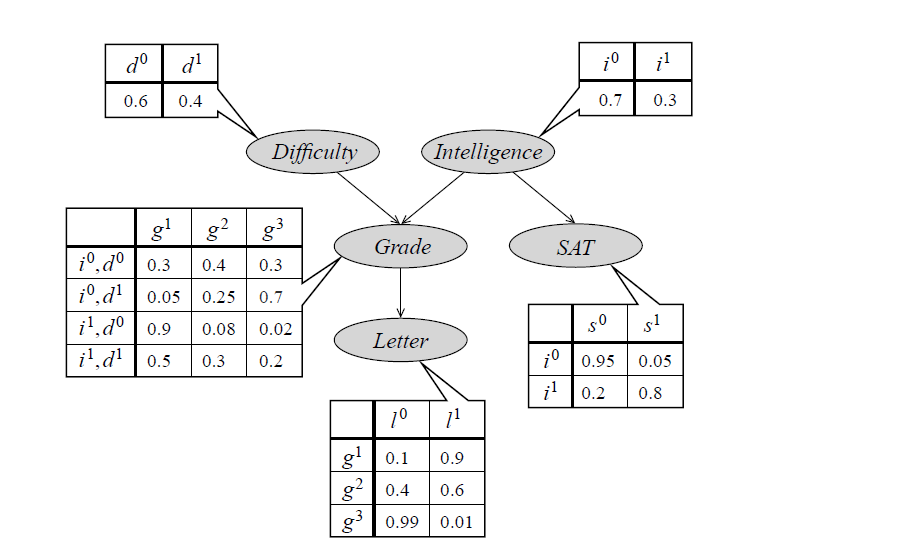
\includegraphics[scale=0.4]{img/bayesianNetworks/bayesianNetworks.png}
    \caption{Red Bayesiana para determinar la inteligencia de un estudiante. Podemos ver que cada nodo tiene una $CPT$ que se calcula en función de sus padres, aquí las variables son ternarias o binarias. Fuente: \cite{probabilisticGraphicalModels}}
    \label{fig:bayesian_network_example}
\end{figure}

 
Este tipo de redes nos ayuda a simplificar el cálculo de distribuciones de probabilidad conjunta. Una de sus propiedades más importantes es la \emph{regla de la cadena}, que proporciona una estructura fundamental para entender cómo las probabilidades conjuntas pueden descomponerse en estas redes. Específicamente, establece que si consideramos que $\aBayesianDistribution$ es una red Bayesiana sobre un conjunto de variables \( \{A_1, \dots, A_n\} \), entonces $\aBayesianDistribution$ especifica una única distribución de probabilidad conjunta \( Pr(U) \), donde \( U = \{A_1, \dots, A_n\} \), que puede expresarse como el producto de todas las CPT's especificadas en $\aBayesianDistribution$. Matemáticamente, se representa como:
\begin{align}\label{eq:bayesian_probability}
    Pr(U) = \prod_{i=1}^{n} P(A_i \mid \text{pa}(A_i))    
\end{align}

donde \( \text{pa}(A_i) \)  denota los padres de \( A_i \) en la red. Esta regla es esencial porque simplifica el cálculo de la distribución de probabilidad conjunta, al descomponerla en dependencias locales más simples entre un nodo y sus predecesores directos. Intuitivamente, lo que hace es utilizar las dependencias locales para definir una distribución global, facilitando los procesos inferencia dentro de estas redes.

%\santi{Acá estamos repitiendo las cosas que ya se dijeron unas páginsa anteriores al hablar por primera vez de redes bayesianas.}

Además, las redes Bayesianas contemplan una variedad de operaciones computacionales cruciales para el razonamiento probabilístico. Una de las operaciones principales es la \textbf{inferencia}, que implica calcular la distribución a priori para alguna variable. Es decir, calcular $Pr(A \mid B_1  \dots B_i)$, siendo $A$ un nodo en la red y $B_i$ otros nodos de la red. Este proceso a menudo se denomina \emph{consulta} a la red. La complejidad de la inferencia depende de la estructura de la red; para redes con forma de polytree (DAG's que su grafo subyacente es un árbol), también conocidas como \emph{simplemente conectadas}, la complejidad es polinomial en el tamaño de las variables de la red \cite{pearl1986bayesianInference}, pero para redes generales la inferencia es $\sharpPhard$. 

%\santi{Hace falta que sean padres? No es en general?} Rta: Es general, pifie

El algoritmo que se utiliza  para realizar la inferencia marginal, cuál es la probabilidad de que una variable tome ciertos valores, es \emph{Variable Elimination} \cite{variableElimination}. Su complejidad depende principalmente del treewidth de la red y puntualmente para redes de un treewidth acotado su complejidad es polinomial respecto al tamaño de la red. En base a esto es que elegimos trabajar con polytrees. 

%\santi{Hace falta poner la explicación de variable elimination? Al final no lo usamos nunca, no?}

\subsection{Predicción promedio en árboles de decision}

Los árboles de decisión son ampliamente utilizados en Inteligencia Artificial (IA) debido a su capacidad para realizar predicciones y clasificaciones basadas en features de los datos de entrada. Al descomponer decisiones en una serie de preguntas y respuestas simples, los árboles de decisión permiten a los usuarios entender el razonamiento detrás de las predicciones del modelo, contribuyendo a la transparencia en sistemas complejos \footnote{Aunque no siempre el camino de un árbol es la mejor explicación, ya que puede haber features redundantes en el camino que no sean claves para la predicción realizada. \cite{audemard2021explanatorypowerdecisiontrees}}.
%\santi{Acá agregaría un footnote y una cita comentando que el camino en el árbol no es necesariamente una buena explicación. Hay discusiones sobre esto en papers de abductive explanations para árboles, por ejemplo \url{https://arxiv.org/pdf/2108.05266} (último párrafo pag 2)}

\begin{definition}
Un \textbf{árbol de decisión} es una estructura jerárquica utilizada para representar funciones de decisión sobre un conjunto finito de variables. Formalmente, un árbol de decisión \(T\) sobre un conjunto de variables \(X\) es un árbol enraizado cuyas componentes principales son:

\begin{itemize}
    \item \textbf{Nodos internos}, cada uno asociado a una variable \(x \in X\) y etiquetado con una condición sobre dicha variable. Estos nodos determinan cómo se bifurcan los datos.
    
    \item \textbf{Ramas}, que conectan un nodo padre con sus hijos y representan los posibles valores o resultados de evaluar la condición del nodo padre.
    
    \item \textbf{Hojas}, que son nodos sin hijos y contienen una salida concreta: una clase, un valor numérico, o una distribución de probabilidad, dependiendo del tipo de problema (clasificación, regresión, o probabilístico).
\end{itemize}

Cada instancia \(e \in ent(X)\), se evalúa recorriendo el árbol desde la raíz hasta una hoja, tomando decisiones en función de las condiciones de los nodos internos. El resultado asociado a la hoja alcanzada es la predicción del modelo para esa instancia.

\end{definition}

Cómo mencionamos previamente, investigamos si el cálculo del promedio era tratable para árboles de decisión con distribuciones de redes bayesianas, ya que nuestro objetivo era calcular ASV en tiempo polinomial. %\santi{Ídem comentario de más arriba. Hacemos esto porque después lo vamos a necesitar para cacular $v(\pi_{<i})$, no por el Teorema 1, que no dice mucho sobre distribuciones no producto.}%\santi{Reescribiría esta oración.}

%\sidesergio{recordar no poner referencias sueltas, poner Teorema ref. Relacionadamente, por consistencia, capitalizar esas referencias (Teorema, Ecuación, etc.)}

%\santi{Sería un poco más formal en la definición.} 

Para este algoritmo\footnote{Pueden encontrar este algoritmo en \path{\pasantia-BICC\asvFormula\bayesianNetworks\bayesianNetwork.py}}, trabajaremos con árboles de decisión binarios, y con features binarios, más adelante veremos la extensión a variables no binarias. Cada nodo determinará un valor para un feature $X_i$, donde el hijo izquierdo corresponde al caso $X_i=0$ y el hijo derecho al caso $X_i=1$. Los features son un conjunto $X$, y su distribución de probabilidad será una red bayesiana $\aBayesianDistribution = (V, E, Pr_B)$. $ev$ y $pathCondition$ son conjuntos de asignaciones $X_i = k$, las cuáles definen que el feature $X_i$ toma el valor $k$. Entonces, $Pr_B(pathCondition \mid ev)$ representa la probabilidad de que dada una instancia que tiene los valores de $ev$, la instancia tome los valores de $pathCondition$, dada la red bayesiana $\aBayesianDistribution$. La idea del algoritmo consiste en explorar todos las ramas e ir acumulando las decisiones tomadas en la variable $pathCondition$. Al llegar a la hoja evaluamos la probabilidad de haber llegado a la hoja, dada la evidencia y la multiplicamos por el valor que la misma devuelve. 

%\santi{Agregaría un párrafo comentando la idea del algoritmo. Aparte, si asumimos que en ningún camino se repiten features podríamos quitar las líneas 2-4, no? Aunque cuando haya más de un valor para cada feature eso deja de ser cierto. Capaz podemos comentarlo (igual no es muy relevante)}

%\santi{Qué es una evidencia? Estás pisando la $E$ de la definición de la red.}

%\echu{No entendí el comentario de Santi de lo de las líneas 2-4}

%Ya se entendio


\begin{algorithm}
\caption{Predicción promedio para árbol de decisión binario} \label{alg:meanPredBinDT}
\begin{algorithmic}[1]
\Function{Mean}{$node$, $B$, $pathCondition$, $evidence$}
    \If{$evidence$ does not match $pathCondition$}
        \State \Return  $0$
    \EndIf
    
    \If{$node$.isLeaf}
        \State \Return  $Pr_B(pathCondition\ | \ evidence)$ * $node.value$
    \EndIf
    \State $X_i \gets n.feature$
    \State $leftMean \gets$  \Call{Mean}{$node$.left, $B$, $pathCondition \cup \set{X_i=0}, evidence$}
    \State $rigthMean\gets$ \Call{Mean}{$node$.right,$B$,$pathCondition \cup \set{X_i=1}, evidence$} 
    \State \Return  \mbox{$leftMean + rigthMean$}
\EndFunction
\end{algorithmic}
\end{algorithm}

Analicemos la complejidad de este algoritmo. La condición del primer \texttt{if} puede ser evaluada en tiempo $O(|V|)$. En las hojas solo hacemos un llamado al algoritmo de \textit{variable elimination}, cuya complejidad denotamos como $O(varElim)$. Por otro lado, en los nodos internos solo se hacen los llamados recursivos extendiendo la \textit{pathCondition}, lo cual puede implementarse en $O(1)$. Por lo tanto, si $l$ denota la cantidad de hojas de nuestro árbol de decisión, e $i$ la cantidad de nodos internos, la complejidad de nuestro algoritmo es $O(i|V| + (varElim)l)$. En el caso de los polytrees $varElim$ es polinomial, por lo que nuestro algoritmo realizaría una cantidad de operaciones polinomial en función del tamaño del árbol de decisión, siendo estas ($O(i + l) = (O(|V|))$) operaciones polinomiales. %, de costo polinomial $O(varElim) \ y \ O(|V|)$.

%\santi{Lineal?}

%\santi{Definir antes que la red es una tupla (V, E, Pr) y acá directamente poner $O(|V|)$}
%\santi{Ojo que cuando hablaste de VE lo consideraste un algoritmo para evaluar $P(A)$, y ahora querés evaluar $P(A | B)$. Podés directamente introducirlo como algo para calcular $P(A|B)$ y obtenés lo otro como caso particular.}
%\santi{Usaría otra expresión distinta a $VE$}

%\santi{Sobre tu comment en el latex, podés no decir polinomial hasta el final, solo poné las complejidades y aclará que VE es polinomial.}

%¿Polinomial en base a que? ¿Aclaro de vuelta todo lo anterior? Siento que estoy diciendo todo el tiempo lo mismo, necesito sinonimos de polinomial. ¿Lo hago más formal?

\begin{figure}[ht]
    \centering
\begin{tikzpicture}[
    level 1/.style={sibling distance=6cm},
    level 2/.style={sibling distance=3cm},
    every node/.style={minimum size=1cm, font=\footnotesize}
]
\node [circle, draw, red] {Letter}
    child {
        node [circle, draw] {Den}
        edge from parent node[left] {\textcolor{red}{$X_0 = 0$}}
    }
    child {
        node [circle, draw, blue] {SAT}
        child {
            node [circle, draw] {Den}
            edge from parent node[left] {\textcolor{blue}{$X_1 = 0$}}
        }
        child {
            node [circle, draw] {Acc}
            edge from parent node[right] {\textcolor{blue}{$X_1 = 1$}}
        }
        edge from parent node[right] {\textcolor{red}{$X_0 = 1$}}
    };
\end{tikzpicture}

    \caption{Decision tree que define si un estudiante va a ser aceptado (accepted/1) o rechazado (denied/0) en su ingreso a una universidad basado en los features de la red bayesiana de la Figura \ref{fig:bayesian_network_example}. Podría ser generado a partir de un dataset con los mismos features de la red, con un feature extra llamado \texttt{Acceptance}. La red usada está en $\backslash pasantia-BICC\backslash networkExamples \backslash student.bif$}
    \label{fig:decision_tree_example}
\end{figure}

%\santi{En el ejemplo deberia haber dos ejes saliendo de Letter (en rojo), o sacar el nodo Letter (en rojo) y solo poner el Den.}

% Tengamos en cuenta que el feature \santi{En general no deberíamos mezclar el target con los features. Entiendo que en la experimentación surgió naturalmente por las redes de ejemplo que tomamos, pero en general para nuestro framework features y valores objetivos son dos cosas complementamente distintas, y no suponemos que tenemos información respecto a su correlación (aunque si la tenemos en nuestros casos de test). Dicho esto, este párrafo no debería estar.} que intentamos predecir no está en nuestra red bayesiana, si este fuera el caso, entonces lo que utilizaríamos para calcular la predicción promedio del feature sería la red misma, no el árbol de decisión.  Rta: Completamente de acuerdo con el comentario, no hace falta esta oración

En la Figura \ref{fig:decision_tree_example} tenemos un ejemplo de un árbol de decisión. Queremos ver cuál es la predicción promedio de nuestro árbol de decisión para un alumno que es inteligente.  Si corremos nuestro algoritmo desde la raíz del árbol, lo que vamos a obtener es
\begin{align*}
        &\Call{Mean}{Letter, B, \{\}, \{INT = 1\}}\\
        &= \Call{Mean}{Den, B, \textcolor{red}{Letter = 0}, \textcolor{brown}{\{INT = 1\}}} + \Call{Mean}{SAT, B, \textcolor{red}{Letter = 1}, \textcolor{brown}{\{INT = 1\}}} \\
        &= 0 + \Call{Mean}{SAT, B, \{Letter = 1\}, \textcolor{brown}{\{INT = 1\}}} \\
        &= \Call{Mean}{Den, B, \{Letter = 0, \textcolor{red}{SAT = 0} \}, \textcolor{brown}{\{INT = 1\}}} + \Call{Mean}{Acc, B, \{Letter = 1, \textcolor{red}{SAT=1}\}, \textcolor{brown}{\{INT = 1\}}} \\
        &=  Pr_B(SAT = 0, Letter = 1\ | \ INT = 1) * 0 +  Pr_B(SAT = 1, Letter = 1\ | \ INT = 1) * 1 \\
        &= Pr_B(SAT = 1, Letter = 1\ | \ INT = 1) \\
        &= 0.61
    \end{align*}

En este ejemplo podemos ver que aunque la inteligencia no sea una variable que se tenga en cuenta en el árbol, afecta la predicción promedio. Ya que para calcularla estamos utilizando la red bayesiana, y esta evidencia introducida va a afectar la inferencia realizada en la red. 

%\santi{Comentario sobre que INT no es una feature usada en el árbol y no obstante afecta la predicción promedio. Digo, porque es algo un poco antiintuitivo, pero es la gracia.}


%\echu{Duda, no se si hacer que las hojas sean  "Denied" y "Accepted" o que sean un "SAT" (o cualquier otra variable) y que ahí te devuelva las probabilidades para cada valor, entiendo que la primera es más "fiel" a lo que buscamos representar.}

%\santi{No entiendo este comentario}

%Respuesta: Deberíamos dejar la primera opción, porque estamos calculando ASV usando 0/1 cómo predicción, no una probabilidad. 

%\santi{Agregar el valor de la predicción esta cuando INT = 0, que es 0.39.} Rta: Al final es 0.019430000000000003, porque es la proba de que (SAT=1 y Letter = 1)

\begin{comment}
    "El código para correr la query. Intelligence puede valer i1 o i0"
    studentNetworkPath = networkSamplesPath + "/student.bif"
    BNmodel = BIFReader(studentNetworkPath).get_model()
    BNInference = VariableElimination(BNmodel)
    query = BNInference.query(evidence={'Intelligence':'i1'}, joint=True, variables = ['Letter', 'SAT'] )
    print(query.get_value(**{'Letter' : 'l1', 'SAT' : 's1'}))
\end{comment}

\subsubsection{Expandiendo la predicción promedio a features no binarios} 

%\echu{¿Juega esta sección?  Santi: Sip, pero muy chill. Contar que no podemos hacer la operación que queremos en la red bayesiana de una forma muy simple y mostrar la forma en la que la implementamos nosotros. }

El Algoritmo \ref{alg:meanPredBinDT} funciona para árboles binarios y para variables binarias. Para poder trabajar con features no binarios tuvimos que modificar la inferencia realizada. Por lo que su complejidad dejo de ser polinomial en el tamaño de la red, ya que la implementación actual depende de la cardinalidad de cada feature.
%\santi{No lo sabemos esto. Habría que saber más de implementaciones de inferencia}. \scc{\sout{Puesto que ahora la cardinalidad de cada feature influye el tiempo que toma}}.

Si cada feature admite más de un valor, cuando llegamos a un nodo $n$ obtenemos su feature $f$ y su umbral de decisión $v$. Luego para los valores $i,d \in Dominio(f)$ se le agregan a $pathCondition$ los $i$ t.q $i<v$ en el lado izquierdo de la recursión y los $d$ t.q $d \geq v$ en el lado derecho. Seguimos realizando la inferencia al llegar al nodo hoja, a través de una suma de la unión de todas las consultas generadas, por lo que la inferencia no es polinomial. Por ejemplo, si llegamos con $pathCondition = \set{x=\set{1,2},y=\set{3}}$ vamos a tener que $Pr_B(pathCondition) = Pr_B(x=1,y=3) + Pr_b(x=2,y=3)$. Para mejorar esta inferencia, una posibilidad sería implementar la consulta modificando el algoritmo de Variable Elimination o creando nodos intermedios que representen la evidencia introducida; pero no tomamos este camino debido a que no es el objetivo principal de esta tesis. 

%\echu{¿Así queda menos en ladri? En respuesta al comentario de Cifu}

%\santi{Hay que sacar esta oración o comentar que existe esta posibilidad. Decir que lo pensamos y no poner nada de resultado me parece ladri.} 

%https://stackoverflow.com/questions/76365165/create-variable-elimination-with-multiple-possible-values-in-pgmpy#:~:text=Unfortunately%2C%20there%20is%20no%20direct,the%20probability%20in%20such%20cases Acá preguntaron lo mismo que nosotros

%\santi{O hacer la query más compleja a la red bayesiana. Yo diría que el algoritmo ahora se reduce a esta query más compleja, que no sabemos si se puede resolver. La oración siguiente a esto solo es la observación de que descomponerla en queries tradicionales no es eficiente, pero capaz no hace falta y se puede manejar de otra forma.}



\begin{comment}
\subsection{Exact mean prediction computation in Decomposable Circuits}

Can we extend the previous algorithm to work in more general models? We can easily prove an upper bound on model complexity related to the satisfiability problem.

\begin{proposition}
    Let $M$ be a model over entities $\entities(X)$ and $\aDistribution$ a distribution over $\entities(X)$ such that no entity has probability 0. Then, deciding if $\expectancy_{e\sim \aDistribution}[M(e)]$ is positive is equivalent to deciding if $M$ is satisfiable.
\end{proposition}

This does not rule out the tractability of exactly computing the average of models for which the satisfiabilily problem is tractable, such as d-DNNF circuits \cite{arenas2021tractability}. For them, we can prove an intractability result exploiting the correlations that one can impose using the Bayesian Network, which allows us to turn a normal Boolean circuit into a d-DNNF one without altering the average prediction.

\begin{proposition}
    The problem of deciding, given a Bayesian distribution $\aBayesianDistribution$ and a d-DNNF circuit $\aCircuit$ whether $\expectancy_{e \sim \aBayesianDistribution}[\aCircuit(e)] > 0$ is \NPhard{}. Moreover, the results holds for Bayesian Networks which are union of disjoint paths.
\end{proposition}

\begin{proof}
    The problem clearly belongs to $\NP{}$, since we can solve it by guessing an entity $e$ such that $\aCircuit(e)$ and $\Pr[e] > 0$. For the hardness, we reduce \textsc{Circuit-SAT} to our problem.

    Let $\aCircuit$ be a Boolean circuit. Without loss of generality we may assume that it is deterministic (i.e. for each $\vee$ gate the two subcircuits $\aCircuit_1$ and $\aCircuit_2$ cannot be simultaneously satisfied). We are going to design a simple Bayesian distribution such that $\aCircuit$ can be understood also as a decomposable circuit.

    We proceed top-down. Let $\wedge$ be the \textit{and} node closest to the top, and let $\aCircuit_1$ and $\aCircuit_2$ the two subcircuits of this node. In principle, $var(\aCircuit_1) \cap var(\aCircuit_2) \neq \emptyset$. To fix this, let $x_1,\ldots, x_k$ be the variables shared by both subcircuits, and replace the variables $x_1,\ldots,x_k$ from $\aCircuit_2$ with the variables $x_1',\ldots,x_k'$. At the same time, we add to the Bayesian network nodes $x_1,x_1',\ldots,x_k,x_k'$ conditioning that whenever $x_i = 1$ then $x_i'=1$ with probability one, and similarly for the case $x_i = 0$, for all $i$.

    Observe that some entities have probability 0: they are exactly those that pick a different value for $x_i$ and $x_i'$, for some $i$. Therefore, if the expected value of this new circuit is positive then there is an assignment of the original circuit such that it is satisfied.

    To complete the reduction we continue working recursively: at each $\wedge$ gate we detect the shared variables $y_1,\ldots,y_\ell$, change them with variables $y_1',\ldots,y_\ell'$ and add the correlations in the Bayesian network $\aBayesianDistribution$.

    Note that the final structure of the Bayesian network is a set of disjoint paths, over which the inference problem be solved easily.
\end{proof}

\subsection{Approximate mean prediction computation}

Even though exact computation is intractable, approximate calculation is straightforward when considering additive precision.

\begin{proposition}
    Let $\aDistribution$ be any distribution over $\entities(X)$ that can be sampled efficiently, and $\mathcal{F}$ a family of models such that evaluating, given $M \in \mathcal{F}$ and $e \in \entities(X)$, the value $M(e)$,q can be done in polynomial time. Then, there is a \textit{Fully Polynomial-time Approximation Scheme} (FPRAS) for $\expectancy_{e \in \aDistribution}[M(e)]$ under additive error\footnote{I don't think we can achieve multiplicative error, looks like satisfiability.}.
\end{proposition}

\begin{proof}
    Note that $M(e) : \aDistribution \to \{0,1\}$ is a random variable bounded between $0$ and $1$ that can be sampled efficiently, and thus the result follows by considering the Hoeffding's inequality.
\end{proof}

\santi{Esto lo podemos escibir juntos la otra semana y ya queda como ejemplo para el otro algoritmo (el de sampleo de ordenes topológicos).}

%Tiene sentido poner que no se puede? Y la demo esa de convertir una red no deterministica en una deterministica en polinomial? O alguna otra justificación?

\end{comment}

\newpage

\section{Optimización para ASV : Clases de equivalencia}\label{Section:HeuristicaASV}
%\echu{Tiene sentido que se llame optimización para ASV? Mejora tal vez sino, pero no me convence. }
%\santi{Capaz le pondría heurísticas. Igual tras leerla veo que esta sección tiene solo herramientas para calcular la cantidad de clases de equivalencia (y en general insight sobre ellas). Capaz el título debería ser ese más que otra cosa.}

\begin{comment}
	Heuristica para ASV
	Introducción
	Cantidad de órdenes topológicos de un DAG
	Queremos topoSorts(polyTree) pues nuestra red es un polytree.
	Cantidad de ordenes topológicos para un “árbol”.
	Cantidad de clases de equivalencia para un “árbol”
\end{comment}


Recordemos la definición de la fórmula de ASV:

\begin{align*}
	\assym_{M,e,\Pr}(x_i) = \sum_{\pi \in \topo(G)} [\charactheristicFunction_{M,e,\Pr}(\pi_{<i} \cup \{x_i\}) - \charactheristicFunction_{M,e,\Pr}(\pi_{<i})] 
\end{align*}

Para simplificar la notación, tomemos $M,e$ y $Pr$ fijos, de modo que $\charactheristicFunction_{M,e,\Pr} = \charactheristicFunction$. La idea es encontrar un criterio para disminuir el número de órdenes topológicos que necesitamos calcular, reduciendo la cantidad de veces que evaluaremos $\charactheristicFunction$. La idea principal detrás de esta heurística es, identificar las clases de equivalencia para los diferentes órdenes topológicos $\toOr^1, \toOr^2 \in \topo(G)$, tales que $\toOr^1 \rel^\star \ \toOr^2 \iff \charactheristicFunction(\toOr^1_{<i}) = \charactheristicFunction(\toOr^2_{<i}) $. Nuestro algoritmo va a trabajar sobre una relación \rel{} más fina que $\rel^\star$, pues esta es costosa de calcular. Al conjunto de clases de equivalencia de $G$ definido por la relación \rel{} lo vamos a denotar como $eqCl(G, x_i)$. Una vez que consigamos todas las clases de equivalencia $\equivalenceClass$, solo necesitamos un representante de cada una y su tamaño para calcular el ASV:

\begin{align*}
	&\assym_{M,e,\Pr}(x_i)\\
	&= \frac{1}{\topo(G)} \sum_{\toOr \in \topo(G)} \charactheristicFunction(\toOr_{<i} \cup \{x_i\}) - \charactheristicFunction(\toOr_{<i}) \\
	&=  \heuristicASVFormula
\end{align*}

%\santi{Por qué $R'$ y no $R$?} \echu{Porque $R$ es la relación "posta" que definimos más adelante, entonces para la que es la ideal use $R'$. Tal vez le podría poner otro nombre, tipo $I$, porque es raro meter un $'$ de la nada. }

%\santi{Ah, entiendo. Capaz pondría $R$ a esta y a la otra $R^\star$, porque el prima acá es raro. Adelantaría en este punto que nuestro algoritmo va a trabajar sobre una clase más fina que esta $R'$ porque no es fácil calcularla} Rta: Todo el sentido del mundo

%Usando nuestra nueva fórmula, las permutaciones que estudiaremos son las de $topo(G)$. Ahora nos vamos a centrar en las clases de equivalencia de $\topo(G)$ siguiendo los criterios definidos anteriormente, teniendo en cuenta que estamos calculando $\phi_{i}^{assym}(\charactheristicFunction)$. \santi{No entiendo a que van estas primeras dos oraciones} $$ Rta: No suman mucha info, las sacamos

\begin{figure}[ht]
	\centering 
	\begin{tikzpicture}[scale=.95, transform shape]
		
		% ---- NODOS ----
		\node[nodo] (a1) at (0, 0) {$a_1$};
		\node[nodo] (a2) at (2.5, 2) {$a_2$};
		\node[nodo] (a3) at (2.5, -2) {$a_3$};
		\node[nodo] (xi) at (5, 0) {$x_i$};
		\node[nodo] (d_1) at (7.5, 2) {$d_1$};
		\node[nodo] (d_2) at (10, -2) {$d_2$};
		\node[nodo] (d_3) at (10, 0) {$d_3$};
		
		\node[draw=none, fill=none] (hijo_a3) at (4.5, -4) {};
		\node[draw=none, fill=none] (hijo_d2) at (8, -4) {};
		
		% ---- ARISTAS ----
		\path [->] (a1) edge[arista, mySnake]  (xi);
		\path [->] (a2) edge[arista, mySnake]  (xi);
		\path [->] (a3) edge[arista, mySnake]  (xi);
		\path [->] (xi) edge[arista, mySnake]  (d_1);
		\path [->] (xi) edge[arista, mySnake]  (d_2);
		\path [->] (xi) edge[arista, mySnake]  (d_3);
		\path [->] (a3) edge[arista, mySnake] node[above right] {descendientes de $a_3$ } (hijo_a3);
		\path [->] (hijo_d2) edge[arista, mySnake] node[below right] {ancestros de $d_2$ } (d_2);
		
	\end{tikzpicture}
	\caption{Al fijar un nodo $x_i$, podemos dividir el resto de los nodos en tres grupos: \textit{ancestros} (todos los nodos que pueden alcanzar a $x_i$), \textit{descendientes} (todos los nodos alcanzables desde $x_i$) y aquellos \textit{no relacionados} con $x_i$. Los \textit{no relacionados} son los que no pertenecen a los ancestros ni a los descendientes, por lo que pueden estar a la derecha o la izquierda de $x_i$ en un orden topológico.}
	\label{fig:unrelatedNodesDefinition}
\end{figure}

%\sergio{Puse en tesis.tex el package caption para hacer que las captions sean más chicas, y así más distinguibles del texto principal. Se puede cambiar}

Sea nuestro DAG $G=(V,E)$, con $A$ el conjunto de ancestros de $x_i$ y $D$ el conjunto de sus descendientes. Podemos ver estos conjuntos representados en la Figura \ref{fig:unrelatedNodesDefinition}. Para este ejemplo introductorio no hay ejes entre los ancestros y descendientes. Para cada orden topológico $\toOr$, sabemos que todo $a \in A$ aparece antes de $x_i$, es decir $\toOr(a) < \toOr(x_i)$, y que todo $d \in D$ aparece después, $\toOr(x_i) < \toOr(d)$. Si esos fueran los únicos nodos a tener en cuenta, entonces $|\topo(G)|= |A|! \cdot |D|!$, es decir, las permutaciones de $A$ multiplicadas por las permutaciones de $D$. Por lo tanto, todos los órdenes tendrían los mismos features fijos antes de $x_i$, $A$, y los mismos después de $x_i$, $D$. Además, todos los órdenes estarían en la misma clase de equivalencia definida por $\rel^\star$, pues el orden de los features en cada permutación $\toOr^1, \toOr^2$ \textit{no afectará el resultado de evaluar} $\charactheristicFunction$, $\charactheristicFunction(\toOr^1) = \charactheristicFunction(\toOr^2)$). Esto nos daría la siguiente fórmula: 
%\santi{Esto medio que asume la estructura del dibujo: que no hay ejes entre los ancestros.}
$$\frac{1}{\topo(G)} \sum_{\toOr \in \topo(G)} [\charactheristicFunction(\toOr_{<i} \cup \{x_i\}) - \charactheristicFunction(\toOr_{<i})] = \frac{|A|! \cdot |D|!}{|A|! \cdot |D|!}  (\charactheristicFunction(\toOr_{<i} \cup \{x_i\}) - \charactheristicFunction(\toOr_{<i})) = \charactheristicFunction(\toOr_{<i} \cup \{x_i\}) - \charactheristicFunction(\toOr_{<i})$$ 
Podemos utilizar cualquier $\toOr \in \topo(G)$ en este caso particular, puesto que todas las evaluaciones de $\charactheristicFunction(\toOr_{<i})$ dan el mismo resultado para cualquier $\toOr$ (puesto que $\set{\toOr_{<i}} = A$). Esto significa que podemos reducir el número de veces que evaluaremos $\charactheristicFunction$, si logramos identificar estas clases de equivalencia. Teniendo en cuenta el caso en el cual tenemos nodos no relacionados, vamos a utilizar la relación \rel{}, en vez de $\rel^\star$, la cual tiene en cuenta a $x_i$, y se define cómo $\toOr^1 \rel \ \toOr^2 \iff \{\toOr^1_{<i}\} = \{\toOr^2_{<i}\}$. Esto nos dice que dos permutaciones están relacionadas por \rel{} si previo a la posición de $x_i$ tienen el mismo conjunto de elementos. Los nodos que nos van a importar son los \textit{no relacionados}, como podemos ver en la Figura \ref{fig:unrelatedNodesDefinition}, estos son los únicos que no van a tener un lugar respecto a $x_i$, definido previamente en base a su posición en el grafo.

%\santi{Podemos borrar esta última parte de oración? Es redundante.} Rta: La oración "puesto que todas las evaluaciones..." es redundante, pero la idea es reforzar ese concepto. Prefiero dejarla
%\santi{El "Así modificamos" viene medio de la nada. Me parece que tiene más sentido comentar primero que si hay nodos no relacionados la cosa se complica, y que en particular por eso cambiamos la clase de equivalencia a esta otra.} Rta: Banco
\begin{definition} \label{equivalenceClassDefinition}
	Sea $G$ un digrafo $G = (V, E)$. Una clase de equivalencia $\equivalenceClass$ define en que posición respecto de $x_i$ se encuentran los nodos de $V$, para un orden topológico $\toOr$. Dada $f_{\toOr}:V \setminus \{x_i\} \to \set{left, right}$, tal que $f_{\toOr}(n)$ es una función que identifica si el nodo $n$ está a la derecha o izquierda de $x_i$ en $\toOr$, la clase  $\equivalenceClass$ se ve representada como un conjunto de nodos con etiquetas $left, right$ según su orden:
	$$
	\equivalenceClassRep = \{ v_{f_{\toOr}(v)} \mid v \in V \setminus \{x_i\} \}
	$$
	
	%\santi{Ojo que el conjunto de arriba tiene TODOS los simbolos de la forma $v_t$ (o sea, tiene $v_{left}$ y $v_{right}$ para todo $v$)}
	
	$L(\equivalenceClass)$ y $R(\equivalenceClass)$ denotan el conjunto de nodos a la izquierda y a la derecha en la clase de equivalencia, respectivamente.
\end{definition}

%\santi{Sea $D=(V,E)$ un digrafo.} \santi{Los nodos de $D$, a.k.a. $V$.} Que hijo de pu que soy
\begin{definition}
	Sea $G$ un digrafo $G = (V, E)$. Un orden topológico $\toOr'$ pertenece a la clase de equivalencia $\equivalenceClass$ si se cumple que: %\santi{Me gusta esta definición, pero seamos más claros con el $f_\pi(n)$} Rta: No se redactar, es terrible
	$$
	(\forall v \in V \setminus \{x_i\}) (f_{\toOr'}(v) = left \land v \in L(\equivalenceClass) ) \lor (f_{\toOr'}(v) = right \land v \in R(\equivalenceClass) )
	$$
\end{definition}

%\santi{Dijiste que $L([\pi]_R)$ es un número y después los usas como conjuntos.} Rta: Upsi, pasas que cosan

Esta es una relación más fina que $\rel^\star$, pues puede pasar que $\toOr^1$ y $\toOr^2$ no estén relacionadas en \rel{} pero sí en $\rel^\star$, por lo que separa en más clases. La ventaja de \rel{} es que no es necesario calcular $\charactheristicFunction$ para saber si dos elementos pertenecen a la misma clase, por lo que nos ahorra evaluaciones. 

%\santi{Mejor "Esta es una relación más fina que...", i.e. separa en más clases.}
\begin{comment}
	\santi{Acá creo que solo hay que poner $\toOr^1_{<i} = \toOr^2_{<i}$, que denota que el conjunto de variables que quedan fijas es el mismo. Pedir esto con el $\charactheristicFunction$ es más laxo pero no sabemos controlarlo.}
	\echu{Pero la idea es justamente que no importe el orden de los elementos tampoco, o sea sólo ver que los conjuntos son iguales}
	\santi{Pero vos no estás pidiendo que los conjuntos sean iguales, sino que pedís que la función evaluada en esos conjuntos lo sea. O sea, hay conjuntos que no son iguales pero a lo mejor si los evaluás te da igual. Ahora mismo escribiste esta última relación.}
	\santi{Quedamos en definir la relación ``ideal'' $R^*$ que captura que dos permutaciones son iguales si dan la misma evaluación. Como eso es difícil, solamente calculamos la relación $R$ que dice que dos permutaciones son iguales si tienen el mismo conjunto de nodos antes del nodo $x_i$.}    
\end{comment}

%\santi{Entiendo la didáctica de presentar primero la propuesta sin considerar los no relacionados, pero me parece mucho escribir la fórmula y todo, porque literal terminas poniendo algo como una ecuación que no querés que quede en la historia. Capaz lo escribiría como: "Dada la relación R, se puede calcular esto como blah blah". Como R nos es dificil de calcular, podemos tomar R', y calcular el shap de la misma forma. Notar que R' se calcula asi y asa en este caso sencillo (sin unrelated) pero en general hay que hacer algo mas complicado (y ahora empieza lo que está abajo, lo importante posta). Igual es como yo lo escribiria, podes ignorarlo.}
%\echu{¿Lo reordene un poco, así te parece que queda bien? En respuesta al comentario descomentado}

%\santi{En el párrafo anterior introduciría estas notaciones que estás usando para referirte al conjunto de clases de equivalencia y a los elementos de ese conjunto (i.e. el coso ese $eqCl(G, x_i)$). Para notar la clase de equivalencia me parece más estándar decir $[\pi]_R$ (esto denota la clase de equivalencia en $R$ a la que pertenece $\pi$). Si lo escribís asi, no tenés que poner el $\pi \in [\pi]_R$ en la expresión :)}

Si podemos calcular el número y tamaño de las clases de equivalencia de manera eficiente, entonces podemos calcular el valor de $ASV$. Para el tamaño de las clases de equivalencia, vamos a calcular el número de órdenes topológicos que pertenecen a la misma. 

\subsection{Número de órdenes topológicos de un DAG}\label{sect:Number Of Toposorts}

Vamos a definir una fórmula para calcular el número de órdenes topológicos de un DAG, la cual va a ser útil para contar los tamaños de las clases de equivalencia. Queremos definir esto para ciertas familias de DAGs, porque sabemos que para el caso general es $\sharpPhard$ \cite{countingLinearExtensions}. Comencemos con el DAG más básico, un grafo $D$ con $r+1$ nodos y sin aristas.

%\santi{Si tiene $n+1$ nodos deberías llamar $h_n$ en vez de $h_r$.}

\begin{figure}[ht]
	\centering 
	\begin{tikzpicture}[scale=.95, transform shape]
		
		% ---- NODOS ----
		\node[nodo] (r) at (0, 0) {$r$};
		\node[nodo] (s1) at (-4, -2) {$h_1$};
		\node[nodo] (s2) at (-2, -2) {$h_2$};
		\node[nodo] (si) at (1, -2) {$h_i$};
		\node[nodo] (sn-1) at (4, -2) {$h_{r}$};
		
		\node[draw=none, fill=none] (dots) at (-0.2, -2) {$\ldots$}; % Ellipsis
		\node[draw=none, fill=none] (dots) at (2.2, -2) {$\ldots$}; % Ellipsis
		
		% \node[draw=none, fill=none] (hijo_a3) at (4.5, -4) {};
		% \node[draw=none, fill=none] (hijo_d2) at (8, -4) {};
		
	\end{tikzpicture}
	\caption{Digrafo vacío, sin aristas}
	\label{fig:emptyGraphExample}
\end{figure}

En la Figura \ref{fig:emptyGraphExample}, el número de órdenes topológicos de $D$ es $r+1!$, porque los nodos no tienen ninguna arista entre ellos, por lo que no hay restricciones. Ahora añadamos algunas aristas a $D$ para que se convierta en un árbol (dirigido) y agreguemos un subárbol debajo de cada nodo $h_j$. Así tenemos la Figura \ref{fig:dtreeExample}.

%\santi{Banco la didáctica. No banco que de una figura a la otra el dibujo es idéntico pero la cantidad de nodos en el segundo piso son distintas ($n$ y $r$). Comentaría algo en el texto para justificar la asimetría (sino parece un typo).}

%\santi{Ojo que estás llamando $s$ a los nodos que tienen nombre $h$ en el dibujo. También, agregar referencia a las figuras (y no confiar que las figuras van a estar bien ubicadas abajo de los párrafos correspondientes)}

\begin{figure}[ht]
	\centering 
	\begin{tikzpicture}[scale=.95, transform shape]
		
		% ---- NODOS ----
		\node[nodo] (r) at (0, 0) {$r$};
		\node[nodo] (s1) at (-4, -2) {$h_1$};
		\node[nodo] (s2) at (-2, -2) {$h_2$};
		\node[nodo] (si) at (1, -2) {$h_i$};
		\node[nodo] (sn-1) at (4, -2) {$h_{r}$};
		
		\node[draw=none, fill=none] (dots) at (-0.2, -2) {$\ldots$}; % Ellipsis
		\node[draw=none, fill=none] (dots) at (2.2, -2) {$\ldots$}; % Ellipsis
		
		\node[draw=none, fill=none] (h1) at (-4, -4) {};
		\node[draw=none, fill=none] (h2) at (-2, -4) {};
		\node[draw=none, fill=none] (hi) at (1, -4) {};
		\node[draw=none, fill=none] (hn-1) at (4, -4) {};
		
		
		\path [->] (r) edge[arista]  (s1);
		\path [->] (r) edge[arista]  (s2);
		\path [->] (r) edge[arista]  (si);
		\path [->] (r) edge[arista]  (sn-1);
		
		\path [->] (s1) edge[arista,  mySnake]  (h1);
		\path [->] (s2) edge[arista,  mySnake]  (h2);
		\path [->] (si) edge[arista,  mySnake]  (hi);
		\path [->] (sn-1) edge[arista,  mySnake]  (hn-1);
	\end{tikzpicture}
	\caption{Polytree con nodos con grados de entrada menores o iguales a 1, lo cual definimos como \dtree.}
	\label{fig:dtreeExample}
\end{figure}

% Misma idea que en https://cs.stackexchange.com/questions/12713/find-the-number-of-topological-sorts-in-a-tree
Aquí la fórmula es recursiva y depende de cada uno de los subárboles de $D$. Ahora tenemos $n+1$ nodos, y los subárboles $t_1, \dots, t_r$ de los hijos $h_1,\ldots,h_r$ tienen $k_1, \dots, k_r$ nodos respectivamente (con $n= k_1 + \dots + k_r$). Sea $\numTopo(r)$ el número de órdenes topológicos del árbol $D$ con raíz $r$. Entonces, la fórmula que tenemos es:
%\santi{Acá se están mezclando las notaciones, no? Los $k_i$ son los que suman $n$. Necesitás los $s_i$? No podés usar directamente los $h_i$?}

$$\numTopo(t) =  \binom{n}{k_1, k_2, \ldots, k_r} \prod_{i=1}^{n} \numTopo(t_i)$$

Podemos combinar los órdenes topológicos de cada hijo, seleccionando en qué posición asignamos a cada uno de ellos. El número de asignaciones diferentes que se pueden hacer en $n$ posiciones con $r$ conjuntos de $k_i$ elementos cada uno es: $ \binom{n}{k_1, k_2, \ldots, k_r}= \frac{n!}{k_1! k_2! \ldots, k_r!}$, el coeficiente multinomial. Ahora, para cada una de esas asignaciones, podemos usar cualquiera de los órdenes topológicos de cada subárbol; eso es él $\prod_{i=1}^{n} \numTopo(t_i)$.
% \santi{Acá de nuevo los $k$ se mezclan con los $s$}

Podríamos intentar añadir más aristas a nuestro DAG $D$, por ejemplo, una arista $(r,d)$ entre $r$ y uno de sus descendientes $d$, como en la Figura \ref{fig:notPolytreeExample}.

\begin{figure}[ht]
	\centering 
	\begin{tikzpicture}[scale=.5, transform shape]
		
		% ---- NODOS ----
		\node[nodo] (r) at (0, 0) {$r$};
		\node[nodo] (s1) at (-4, -2) {$s_1$};
		
		\node[draw=none, fill=none] (h1) at (-4, -4) {};
		
		\path [->] (r) edge[arista]  (s1);
		\draw[->] (r) to[bend left] (h1);
		
		
		\path [->] (s1) edge[arista,  decorate, decoration={snake, amplitude=.4mm, segment length=4mm, post length=1mm}]  (h1);
		
	\end{tikzpicture}
	\caption{Arista entre descendiente de $s1$ y $r$}
	\label{fig:notPolytreeExample}
\end{figure}

Pero dejaría de ser un polytree, pues introduciría un ciclo en el grafo no dirigido, y queremos limitarnos a contar los órdenes de este tipo de grafos. Algo que sí podemos añadir son múltiples raíces $r_1, \dots, r_l$ en nuestro grafo, lo que seguiría siendo un polytree (o un polyforest). Y podemos calcular el \numTopo \ añadiendo una raíz \emph{virtual} $r_0$ que esté conectada a todas ellas, para luego usar la misma fórmula como si fuera un árbol. Esto lo podemos observar en la Figura \ref{fig:topoSortCalcForForests}.

\begin{figure}[ht]
	\centering 
	\begin{tikzpicture}[scale=.95, transform shape]
		
		% ---- NODOS ----
		\node[nodo, blue] (r) at (0, 0) {$r_0$};
		\node[nodo] (s1) at (-4, -2) {$r_1$};
		\node[nodo] (s2) at (-2, -2) {$r_2$};
		\node[nodo] (si) at (1, -2) {$r_i$};
		\node[nodo] (sn-1) at (4, -2) {$r_{l}$};
		
		\node[draw=none, fill=none] (dots) at (-0.2, -2) {$\ldots$}; % Ellipsis
		\node[draw=none, fill=none] (dots) at (2.2, -2) {$\ldots$}; % Ellipsis
		
		\node[draw=none, fill=none] (h1) at (-4, -4) {};
		\node[draw=none, fill=none] (h2) at (-2, -4) {};
		\node[draw=none, fill=none] (hi) at (1, -4) {};
		\node[draw=none, fill=none] (hn-1) at (4, -4) {};
		
		
		\path [->] (r) edge[arista, blue]  (s1);
		\path [->] (r) edge[arista, blue]  (s2);
		\path [->] (r) edge[arista, blue]  (si);
		\path [->] (r) edge[arista, blue]  (sn-1);
		
		\path [->] (s1) edge[arista,  decorate, decoration={snake, amplitude=.4mm, segment length=4mm, post length=1mm}]  (h1);
		\path [->] (s2) edge[arista,  decorate, decoration={snake, amplitude=.4mm, segment length=4mm, post length=1mm}]  (h2);
		\path [->] (si) edge[arista,  decorate, decoration={snake, amplitude=.4mm, segment length=4mm, post length=1mm}]  (hi);
		\path [->] (sn-1) edge[arista,  decorate, decoration={snake, amplitude=.4mm, segment length=4mm, post length=1mm}]  (hn-1);
	\end{tikzpicture}
	\caption{El DAG original son los nodos y aristas en negro, el nodo virtual y sus aristas están en azul.}
	\label{fig:topoSortCalcForForests}
\end{figure}

Si tenemos múltiples raíces, entonces podría suceder que compartan algunos descendientes comunes. Pero si dos raíces $r_i$ y $r_j$ comparten dos o más descendientes $d_1$ y $d_2$, tales que hay dos caminos disjuntos de 
$r_i$ a $d_k$ y $r_j$ a $d_k$, con $k \in \set{1,2}$, entonces va a existir un ciclo en el grafo: $r_i \to d_1 \to r_j \to d_2 \to r_i$, por lo que no sería un polytree. Eso implica que dos raíces solo pueden compartir uno de estos nodos como máximo, puesto que sino el grafo subyacente va a tener un ciclo. Por ejemplo, este sería un polytree válido, como en la Figura \ref{fig:polyTreeNotDTreeExample}.

%\santi{Ojo que en el dibujo comparten todos los descendientes por debajo de $s_2$. La condición que hay que expresar es un toque más complicada, algo asi como que hay un solo nodo tal que hay dos caminos disjuntos de $r_1$ y de $r_2$ a ese nodo.}

\begin{figure}[ht]
	\centering 
	\begin{tikzpicture}[scale=.95, transform shape]
		
		% ---- NODOS ----
		\node[nodo] (r1) at (-2,0) {$r_1$};
		
		\node[nodo] (r2) at  (2,0) {$r_2$};
		
		\node[nodo] (s1) at (-2,-2) {$s_1$};
		\node[nodo] (s2) at (0,-2) {$s_2$};
		\node[nodo] (s3) at (2,-2) {$s_3$};
		
		
		\node[draw=none, fill=none] (h1) at (-2, -4) {};
		\node[draw=none, fill=none] (h2) at (0, -4) {};
		\node[draw=none, fill=none] (h3) at (2, -4) {};
		
		
		\path [->] (r1) edge[arista]  (s1);
		\path [->] (r1) edge[arista]  (s2);
		\path [->] (r2) edge[arista]  (s2);
		\path [->] (r2) edge[arista]  (s3);
		
		\path [->] (s1) edge[arista,  decorate, decoration={snake, amplitude=.4mm, segment length=4mm, post length=1mm}] (h1);
		\path [->] (s2) edge[arista,  decorate, decoration={snake, amplitude=.4mm, segment length=4mm, post length=1mm}]  (h2);
		\path [->] (s3) edge[arista,  decorate, decoration={snake, amplitude=.4mm, segment length=4mm, post length=1mm}]  (h3);
		
		
		\path [->] (s2) edge[arista,  decorate, decoration={snake, amplitude=.4mm, segment length=4mm, post length=1mm}]  (h2);
	\end{tikzpicture}
	\caption{Ejemplo de polytree, para el cual no funciona la fórmula \ref{for:topoCountingDTrees} para contar los órdenes topológicos en \dtrees}
	\label{fig:polyTreeNotDTreeExample}
\end{figure}

En este caso, no podemos usar la misma fórmula que para el árbol, porque hay un solapamiento entre los descendientes de $r_1$ y $r_2$. Sabemos que no puede haber ninguna arista entre los subárboles de $s_1$, $s_2$ y $s_3$, porque eso crearía un ciclo. Para resolver este caso más general, polytrees, tuvimos que implementar una solución más compleja, entraremos más en detalle acerca de la misma en la sección \ref{Section:SampleoToposorts}. Por el momento, simplemente vamos a trabajar con el caso resuelto previamente, el cual engloba polyforests con nodos con un padre como máximo. A estos los llamaremos \dtrees \ (directed trees).
%\santi{Voto cambiar todos los meramente por simplemente (opinionated)} Rta: Ahí los cambie todos, excepto uno
%\echu{ Revisar el nombre. ¿Dforests sino puede ser? }
%\santi{Podría ser. No se igual si hay un nombre estándar. Por las dudas, estaría bueno aclarar en la intro o un lugar donde decimos lo que se hizo que esta heurística es solo para el caso de dtrees (capaz ya está dicho, dejo el comment para no olvidarnos)}

%\santi{Capaz podemos sacar esta discusión. Directamente podemos poner "Prop 1: dado un dtree, su cantidad de ordenes topológicos es .... Corolario 2: un dtree disconexo tiene tantos ordenes topológicos. Mini Discusión: No pudimos extender esto a no dtrees. Siento que está medio largo ahora, y vueltero.}
%\echu{Lo modifique ¿Así queda mejor o sigue siendo muy vueltero? En respuesta al comentario descomentado}

La fórmula que tenemos entonces es: 

\begin{definition}\label{for:topoCountingDTrees}
	Dado un \dtree{} $t$, con $n$ subárboles $t_i$, cada uno de tamaño $k_i$, la cantidad de órdenes topológicos del mismo es: 
	\begin{align}
		\numTopo(t) =  \binom{n}{k_1, k_2, \ldots, k_r} \prod_{i=1}^{n} \numTopo(t_i)  
	\end{align}
\end{definition}


Analizando esta fórmula, podemos observar que:

\begin{itemize}
	\item Para minimizar la cantidad de órdenes topológicos, es mejor tener una cantidad de subárboles pequeña. %\santi{Esto me parece un stretch, ya que necesitas que los $k_i$ sean grandes pero también que la productoria esté controlada. Pondría solo que es mejor que haya menos subárboles (que es lo mismo que decir que algunos $k_i$ son grandes}
	% \item Si tenemos un grado máximo de salida $m$ lo suficientemente pequeño, entonces sabemos que para cada nivel, el mayor $k$ (tamaño del subárbol) estará acotado por $\frac{n}{m}$. \santi{No entiendo del todo a qué se refiere esto} Echu: Es falso, quería poner una cota al tamaño del subárbol. Pero podes tener un grado de salida pequeño y que todos los nodos se concentren en uno de los subárboles. 
	\item Si el grado máximo de salida $m$ es lo suficientemente pequeño, entonces las combinaciones que vamos a realizar en el multinomial también van a ser pocas. %\santi{Este punto es muy parecido al anterior, no?} Rta: Es similar, pero no exactamente lo mismo. 
	
	\item La cantidad de órdenes está acotada por $n!$, y este es el caso en el cuál no tenemos ningún arista en el bosque. 
	%\item Si tenemos un árbol compuesto por múltiples caminos de una longitud razonable, entonces el número de órdenes topológicos podría ser tratable. \echu{ Revisar esta última afirmación. } Echu: Medio fruteli
	
\end{itemize}

\subsection{Número de clases de equivalencias para \dtrees} %¿Or polytree?

Con nuestra nueva definición de clase de equivalencia, la idea es calcular el número de clases de equivalencia de un DAG. Como se mencionó previamente, lo que vamos a analizar son los \emph{nodos no relacionados} (unrelated) $U$ y las distintas restricciones entre ellos. Estos son los nodos que no son descendientes ni ancestros de $x_i$ (el feature para el cual estamos calculando el $ASV$). Comencemos con el caso de calcular el número de clases de equivalencia $\equivalenceClass$ para un \dtree con el feature $x_i$.

\begin{figure}[ht]
	\centering 
	\begin{tikzpicture}[scale=.95, transform shape, 
		unrelated/.style={circle, draw=red},
		wiggly/.style={decorate, decoration={snake, amplitude=.2mm, segment length=2mm}}  % Define wiggly line style
		]
		
		
		% ---- NODOS ----
		\node[nodo, blue] (r) at (0, 0) {$r$};
		\node[unrelated] (a1) at (-1, -2) {$a_1$};
		\node[nodo, blue] (a2) at (1, -2) {$a_2$};
		
		\node[unrelated] (b1) at (-1, -4) {$b_1$};
		\node[nodo, blue] (b2) at (1, -4) {$b_2$};
		\node[unrelated] (b3) at (3, -4) {$b_3$};
		
		\node[unrelated] (c1) at (0, -7) {$c_1$};
		\node[nodo, blue] (c2) at (3, -6) {$c_2$};
		
		\node[nodo] (xi) at (3, -8) {$x_i$};
		
		
		
		\node[draw=none, fill=none] (hi) at (3, -10) {};
		
		
		\path [->] (r) edge[arista]  (a1);
		\path [->] (r) edge[arista]  (a2);
		
		\path [->] (a2) edge[arista]  (b1);
		\path [->] (a2) edge[arista]  (b2);
		\path [->] (a2) edge[arista]  (b3);
		
		\path [->] (b2) edge[arista]  (c1);
		\path [->] (b2) edge[arista]  (c2);
		
		\path [->] (c2) edge[arista]  (xi);
		
		
		\node[text=red] at (-2, -8) {$c_1$ subtree}; 
		\draw[red, wiggly] (-1, -9) -- (0,-7.4) -- (1, -9) -- cycle;  % Draw the triangle
		
		\node[text=red] at (-3, -5) {$b_1$ subtree}; 
		\draw[red, wiggly] (-2, -6) -- (-1,-4.4) -- (0, -6) -- cycle;  % Draw the triangle
		
		\path [->] (xi) edge[arista,  decorate, decoration={snake, amplitude=.4mm, segment length=4mm, post length=1mm}] node[right] {descendants of $x_i$} (hi);
	\end{tikzpicture}
	\caption{Ejemplo de un \ \dtree \ con $x_i$ en negro, sus nodos no relacionados marcados en rojo y sus ancestros marcados en azul.}
	\label{fig:dtreeForestForEquivalenceClasses}
\end{figure}

En el caso de la Figura \ref{fig:dtreeForestForEquivalenceClasses}, los nodos relevantes son los que están en rojo. Esto se debe a que los descendientes de $x_i$ siempre estarán a la derecha de $x_i$ en cualquier orden topológico y sus ancestros aparecerán a la izquierda, por lo que no definirán nuevas clases de equivalencia. Si no hubiera ningún eje en los nodos de $U$, entonces el número de clases sería $2^{|U|}$ \footnote{Sólo queremos contabilizar las clases de equivalencia no vacías, por lo que deben tener al menos un orden topológico que pertenezca a la misma. Por lo que, por ejemplo, no vamos a tener en cuenta a clases con los ancestros de $x_i$ a la derecha.}, debido a que para definir un orden solo se necesita definir dónde insertar los nodos de $U$. Pero si no tienen ninguna arista que los conecte, entonces cada uno de ellos puede colocarse a la izquierda o a la derecha de $x_i$ independientemente del resto, definiendo una nueva clase de equivalencia. Podemos observar que al no haber ejes entre los subárboles de $b_1$ y $c_1$, cada forma posible de ordenar los nodos de $b_1$ se puede mezclar con cada forma de $c_1$ (siempre respetando que $c_1$ aparezca luego de $b_2$). Gracias a esta observación es que podemos calcular los posibles órdeness topológicos y las respectivas clases de equivalencia de cada subárbol de nodos no relacionados, para luego combinar estos resultados. ¿Cómo podemos calcular estas clases de equivalencia, considerando solo los nodos del subárbol, para cada uno?
%¿Qué ocurre cuando algunos de estos nodos no relacionados tienen descendientes o están conectados a algún ancestro/descendiente?
%\santi{Ningún eje} 
%\santi{Capaz acá está bueno hablar un poco de independencia: como entre dos subárboles $b_1$ y $c_1$ no hay ejes, cada posible forma de organizar los nodos de $b_1$ puede mezclarse con cualquier forma de organizar los nodos de $c_1$ (parcialmente, ya que todavía hay que respetar que $b_2$ tiene que aparecer antes que $c_1$. Es por esto que nos resulta útil contar las clases de equivalencia de cada subárbol.}

%\santi{Ojo que no estás contando las clases de equivalencia, eso está definido como otra cosa. Acá estas contando cuántas formas hay de partir los nodos en dos conjuntos $L$ y $R$ de tal forma que ningún nodo de $R$ sea ancestro de alguno de $L$. Igual es verdad que lo podés pensar como clases de equivalencia, pero sería sobre otra red causal que solo tiene al subárbol de unrelated y al nodo $x_i$. Tener cuidado, asi como está escrito no es claro, y como no hay demostraciones esto tiene que estar clarísimo.}

\begin{figure}[ht]
	\centering 
	\begin{tikzpicture}[scale=.95, transform shape, 
		unrelated/.style={circle, draw=red},
		wiggly/.style={decorate, decoration={snake, amplitude=.2mm, segment length=2mm}}
		]
		
		% ---- NODOS ----
		\node[unrelated] (b1) at (0, 0) {$b_1$};
		\node[unrelated] (11) at (-1, -2) {$1_1$};
		\node[unrelated] (12) at (1, -2) {$1_2$};
		
		\node[unrelated] (21) at (-1, -4) {$2_1$};
		\node[unrelated] (22) at (1, -4) {$2_2$};
		\node[unrelated] (23) at (3, -4) {$2_3$};
		
		% ---- ARISTAS ----
		\path [->, draw=red] (b1) -- (11);
		\path [->, draw=red] (b1) -- (12);
		\path [->, draw=red] (11) -- (21);
		\path [->, draw=red] (12) -- (22);
		\path [->, draw=red] (12) -- (23);
		
		% ---- LÍNEA DE CORTE ----
		\draw[dashed, thick] (-2, -3.1) -- (4, -3.1);
		
		% ---- ETIQUETAS ----
		\node at (-2.2, -2.5) {\small \textbf{Izquierda}};
		\node at (-2.2, -3.7) {\small \textbf{Derecha}};
		
	\end{tikzpicture}
	\caption{Ejemplo de una clase de equivalencia para los nodos del subárbol de $b_1$ en la Figura \ref{fig:dtreeForestForEquivalenceClasses}, que divide los nodos en aquellos ubicados a la izquierda o a la derecha de $x_i$ en un orden topológico. En este caso la clase sería $L(\equivalenceClass) = \set{b_1, 1_1, 1_2}, R(\equivalenceClass) = \set{2_1, 2_2, 2_3}$}
	\label{fig:unrelatedSubtree}
\end{figure}


Para responder esta pregunta calculemos el número de clases de equivalencia para uno de los subárboles. Tomemos la Figura \ref{fig:unrelatedSubtree} como el subárbol $b_1$ del ejemplo anterior. Nuestro objetivo es calcular el número de clases de equivalencia del subárbol con raíz en $b_1$, $\numEqCl(b_1)$. Para $b_1$, tenemos dos opciones: puede ser posicionado a la derecha o a la izquierda de $x_i$ en el orden topológico $\toOr$. Si se posiciona a la derecha, entonces todos sus descendientes también estarán posicionados a la derecha, pues deben aparecer luego de $b_1$. Si se posiciona a la izquierda, entonces no hay ninguna restricción sobre sus descendientes. Entonces, nuestra fórmula sería:
$$\numEqCl(b_1) = \numEqCl(b_1 | \toOr(b_1) > \toOr(x_i) ) +  \numEqCl(b_1 | \toOr(b_1) < \toOr(x_i) )  = 1 + \numEqCl(b_1 | \toOr(b_1) < \toOr(x_i) ) $$

%\santi{Estaría bueno un dibujo acá contando a qué nos referimos con clase de equivalencia del árbol. Sobre el mismo dibujo podes dibujar una línea y decir que la clase queda definida por los nodos arriba de la línea y los de abajo.}

$\numEqCl(b_1 | \toOr(b_1) > \toOr(x_i) )$ lo sustituimos por 1, ya que los elementos a la izquierda de $x_i$ van a ser los mismos para todos esos órdenes topológicos, puesto que sus descendientes van a estar a la derecha, por lo que todos los órdenes topológicos con $b_1$ a la derecha van a pertenecer a la misma $\equivalenceClass$.
Ahora, si $b_1$ está posicionado a la izquierda de $x_i$, entonces no hay restricciones para sus hijos ni sus subárboles, y podemos aplicar el mismo proceso para cada uno de sus hijos. Luego, podemos combinar cada $\equivalenceClass$ obtenida en los subárboles, puesto que no tienen aristas en común. En términos de combinatoria, eso significa multiplicar el resultado que obtenemos para cada subárbol. También debemos tener en cuenta el caso en el que el nodo no tiene hijos; ahí podemos tener dos clases de equivalencia, considerando las posibilidades de izquierda y derecha. Así es como obtenemos esta fórmula:

\begin{formula}\label{formula:number_of_equiv_classes}
	Dado un nodo $n$ de un subárbol, la cantidad de clases de equivalencia con respecto a $x_i$ se calcula como:
	$$    \numEqCl(n) = 
	\begin{cases} 
		2 & \text{si $n$ es una hoja} \\
		\prod_{c \in children(n)} \numEqCl(c) + 1 & \text{oc.}
	\end{cases}
	$$
	
\end{formula}


%\santi{Sacar el ingles de la fórmula}
Esta fórmula también puede usarse para calcular las clases de equivalencia de todos los nodos \emph{no relacionados} en el ejemplo anterior. Podemos usar una estrategia similar a la utilizada para calcular los órdenes topológicos. Creamos un nodo $r_0$ y lo conectamos a las raíces de todos los subárboles de los nodos no relacionados, y luego calculamos $\numEqCl(r_0)$ utilizando la fórmula definida previamente. 

\begin{figure}[ht]
	\centering 
	\begin{tikzpicture}[scale=.95, transform shape, 
		unrelated/.style={circle, draw=red},
		wiggly/.style={decorate, decoration={snake, amplitude=.2mm, segment length=2mm}}  % Define wiggly line style
		]
		
		
		% ---- NODOS ----
		\node[nodo] (r) at (0, 0) {$r$};
		\node[nodo, draw=blue] (r0) at (4, 0) {$r_0$};
		\node[unrelated] (a1) at (-1, -2) {$a_1$};
		\node[nodo] (a2) at (1, -2) {$a_2$};
		
		\node[unrelated] (b1) at (-1, -4) {$b_1$};
		\node[nodo] (b2) at (1, -4) {$b_2$};
		\node[unrelated] (b3) at (3, -4) {$b_3$};
		
		\node[unrelated] (c1) at (0, -7) {$c_1$};
		\node[nodo] (c2) at (3, -6) {$c_2$};
		
		\node[nodo] (xi) at (3, -8) {$x_i$};
		
		
		
		\node[draw=none, fill=none] (hi) at (3, -10) {};
		
		
		\path [->] (r) edge[arista]  (a1);
		\path [->] (r) edge[arista]  (a2);
		
		\path [->] (a2) edge[arista]  (b1);
		\path [->] (a2) edge[arista]  (b2);
		\path [->] (a2) edge[arista]  (b3);
		
		\path [->] (b2) edge[arista]  (c1);
		\path [->] (b2) edge[arista]  (c2);
		
		\path [->] (c2) edge[arista]  (xi);
		
		\path [->] (r) edge[arista]  (a1);
		\path [->] (r0) edge[arista, draw=blue]  (a1);
		\path [->] (r0) edge[arista, draw=blue]  (b1);
		\path [->] (r0) edge[arista, draw=blue]  (b3);
		\path [->] (r0) edge[arista, draw=blue]  (c1);
		
		\node[text=red] at (-2, -8) {$c_1$ subtree}; 
		\draw[red, wiggly] (-1, -9) -- (0,-7.4) -- (1, -9) -- cycle;  % Draw the triangle
		
		\node[text=red] at (-3, -5) {$b_1$ subtree}; 
		\draw[red, wiggly] (-2, -6) -- (-1,-4.4) -- (0, -6) -- cycle;  % Draw the triangle
		
		\path [->] (xi) edge[arista,  decorate, decoration={snake, amplitude=.4mm, segment length=4mm, post length=1mm}] node[right] {descendants of $x_i$} (hi);
	\end{tikzpicture}
	\caption{Estrategia utilizada para calcular las clases de equivalencia de los nodos no relacionados, no de todo el DAG.}
\end{figure}

%\santi{Este párrafo biene un poco de la nada, el lector no sabe que el algoritmo tiene complejidad proporcional a las clases (o si?)}

En la sección siguiente se presenta un algoritmo para obtener las clases de equivalencia, el cual es polinomial en la cantidad de clases. Por lo que utilizando la Fórmula \ref{formula:number_of_equiv_classes}, podemos prever el tiempo que va a tomar obtener las clases de equivalencias, puesto que ya tenemos una cota para las mismas. Esta fórmula la podemos correr en tiempo polinomial para realizar una aproximación del tiempo que va a tardar. %\santi{Mejorar mucho este párrafo, la redacción esta rarísima. Hay muchos puntos.}
\begin{comment}
	Hay un caso que no estamos considerando, y es cuando los nodos no relacionados tienen ancestros. Pero ese es el mismo caso para el cual \emph{no pudimos encontrar una respuesta} en el conteo de los ordenes topológicos. En este caso, sería fácil solucionarlo, ya que solo necesitarías conectar $r_0$ a la nueva raíz del subárbol. El problema surge si el subárbol tiene múltiples raíces, entonces la fórmula que definimos anteriormente no sería suficiente, porque estaría contando algunos escenarios dos veces.    
	Al final no lo agregué, no suma tanto. 
\end{comment}

\subsection{Cota superior para las clases de equivalencia}

Queremos encontrar una cota superior para el número de clases de equivalencia de un árbol, para ver si el número de clases de equivalencia será menor que los posibles órdenes topológicos y si es que esta heurística trae consigo una mejora significativa. 

\begin{lemma}\label{lemma:upper_bound_equivalence_classes}
	Sea  $T$ un árbol con su raíz $n$, donde $l$ es el número de hojas del árbol y $h$ es su altura. Entonces, para la fórmula: 
	\[
	\numEqCl(n) = 
	\begin{cases} 
		2 & \text{if $n$ is a leaf} \\
		\prod_{c \in children(n)} \numEqCl(c) + 1 & \text{oc.}
	\end{cases}
	\]
	tenemos la cota $\numEqCl(n) \leq h^l + 1$
	
\end{lemma}

La demostración está en el apéndice en la sección \ref{subsubSection:proofUpperBoundEquivalenceClasses}. Con esta cota podemos observar que: 
\begin{itemize}
	\item Si el número de hojas es $O(\log n)$ y la altura del árbol es $O(n)$, entonces el número de clases de equivalencia está acotado por $O(n^{\log n})$. Esta cota es \emph{subexponencial}. %\santi{Esto no es exponencial. Podés decir que no es exponencial, pero tampoco polinomial (o sea, un punto medio).}, con la cota $O(n^{\log n})$. 
	\item Si la cantidad de hojas es pequeña, entonces nuestra cota va a disminuir también. Lo que significa que es mejor tener un pequeño grado de salida desde cada vértice, al igual que con los órdenes topológicos. %\santi{No me gusta nada el queremos en general. Diría directamente "Si hay pocas hojas el valor de la cota es mejor, asi que nice"}
	\item Es mejor tener una mayor altura que un grado de salida mayor con mucha ramificación.
	\item La cota para el número de clases de equivalencia depende de $h$ y $l$, a diferencia de la cota para los órdenes topológicos que solo depende de $n$, $O(n!)$. Más adelante veremos la diferencia en la práctica.
\end{itemize}


\section{Algoritmo exacto para clases de equivalencia en \ \dtrees}\label{Section:AlgoritmoEquivClasses}

%\santi{En general me gustaría replantear esta sección, eligiendo notación que haga más conveniente las expresiones. Me refiero a escribir en el pizarrón qué cosas tienen que estar, y asi quitarle las que estén de más. Ahora mismo siento que es más difícil de entender de lo que debería.} Rta: Lo charlamos en la llamada del 17/04 y replanteamos algunas cosas


	% ------------------------------------------------
\begin{frame}{Cálculo de ASV}
	\dificultyLevel{2}	
	Ahora queremos calcular ASV utilizando nuestra heurística:
	\only<1>{$$\assym_{M,e,\Pr}(x_i) = \heuristicASVFormula$$ } 
	\only<2>{$$\assym_{M,e,\Pr}(x_i) =\frac{1}{|\topo(G)|} \sum_{\alert{\equivalenceClass \in eqCl(G, x_i)}} (\charactheristicFunction(\toOr_{<i} \cup \{x_i\}) - \charactheristicFunction(\toOr_{<i})) * |\equivalenceClass|$$
		
		¿Cómo obtenemos las clases de equivalencia? }
	
	\end{frame}
	
\begin{comment}
		\item Primero necesitamos obtener el conjunto de clases de equivalencia $eqCl(G,x_i)$ y sus tamaños.
	\item Luego vamos a elegir un representante  por clase para evaluar la sumatoria.
	
	% ------------------------------------------------
	\begin{frame}[fragile]{Solución Naive}
		\dificultyLevel{3}
		\begin{algorithm}[H]
			\caption{NaiveEquivClasses($G$, $x_i$)} \label{alg:naiveAlgorithm}
			\begin{enumerate}
				\item $\mathit{orders} \leftarrow$ generarTodosLosOrdenesTopologicos($G$)
				\item Inicializar diccionarios \texttt{classes} y \texttt{classesSizes}
				\item Para cada $\pi \in \mathit{orders}$:
				\begin{enumerate}
					\item $U_{\pi} \leftarrow$ nodos no relacionados antes de $x_i$ en $\pi$
					\item Agregar $\pi$ a \texttt{classes}[$U_{\pi}$]
				\end{enumerate}
				\item Para cada clase $C$ en \texttt{classes}:
				\begin{enumerate}
					\item $\mathit{rep} \leftarrow$ first(\texttt{classes}[C])
					\item $\mathit{size} \leftarrow$ |\texttt{classes}[C]|
					\item \texttt{classesSizes}[$U_{\pi}$] $\leftarrow (rep, size, C)$
				\end{enumerate}
			\end{enumerate}
		\end{algorithm}
		\vspace{1ex}
		\textbf{Complejidad:} $O(n!)$ en el peor caso (todos los órdenes posibles).
	\end{frame}
\end{comment}

\begin{frame}{Solución Naive}
	\dificultyLevel{2}
	\begin{itemize}[<+- | alert@+>]
		\item \textbf{Generar todos los órdenes} topológicos $\mathit{orders}=\topo(G)$.
		\item Agrupar cada $\pi\in\mathit{orders}$ según 
		$U_\pi=$, sus nodos no relacionados antes de $x_i$.
		\item Para cada grupo $U_\toOr$, guardar un representante y su tamaño.
		\item \textbf{Complejidad:} $O(n!)$ en el peor caso.
	\end{itemize}
\end{frame}
	
	% ------------------------------------------------
	\begin{frame}{Algoritmo Recursivo}
	\dificultyLevel{2}
		\begin{itemize}[<+- | alert@+>]
			\item Etiquetar $G$ como:
			\begin{enumerate}
				\item Ancestros $A$ de $x_i$.
				\item Descendientes $D$ de $x_i$.
				\item Árboles no relacionados (raíces $UR$).
			\end{enumerate}
			\item Paso 1: calcular las clases de equivalencia para todos los subárboles no relacionados.
			\item Paso 2: fusionar los resultados obtenidos con $A$ y $D$.
		\end{itemize}
	\end{frame}
	
	% ------------------------------------------------
	\begin{frame}{Ejemplo: Grafo Etiquetado}
	\dificultyLevel{2}
		\begin{figure}[H]
			\centering
			 \begin{tikzpicture}[scale=.5, transform shape, 
				unrelated/.style={circle, draw=red},
				ancestor/.style={circle, draw=blue},
				]
				\node[text=blue, font=\Large] at (-5, 0) {Ancestros};
				\node[text=teal, font=\Large] at (-5, -0.5) {Descendientes};
				\node[text=red, font=\Large] at (-5, -1) {No relacionados};        
				
				% ---- NODOS ----
				
				\node[ancestor] (a1) at (0, 0) {$a_1$};
				\node[unrelated] (u1) at (-1, -2) {$u_1$};
				\node[ancestor] (a2) at (1, -2) {$a_2$};
				
				\drawUnrelatedTree{u2}{-1}{-4}{$u_2$}
				\node[ancestor] (a3) at (1, -4) {$a_3$};
				\node[unrelated] (u3) at (3, -4) {$u_3$};
				
				\drawUnrelatedTree{u4}{0}{-7}{$u_4$}
				\node[ancestor] (a4) at (3, -6) {$a_4$};
				
				\node[nodo, font=\Large] (xi) at (3, -8) {$x_i$};
				
				\drawUnrelatedTree{r1}{6}{0}{$u_5$} 
				\drawUnrelatedTree{r2}{10}{0}{$u_6$} 
				
				\node[draw=none, fill=none] (hi) at (3, -10) {};
				
				
				\path [->] (a1) edge[arista]  (u1);
				\path [->] (a1) edge[arista]  (a2);
				
				\path [->] (a2) edge[arista]  (u2);
				\path [->] (a2) edge[arista]  (a3);
				\path [->] (a2) edge[arista]  (u3);
				
				\path [->] (a3) edge[arista]  (u4);
				\path [->] (a3) edge[arista]  (a4);
				
				\path [->] (a4) edge[arista]  (xi);      
				\path [->, teal] (xi) edge[arista,  decorate, decoration={snake, amplitude=.4mm, segment length=4mm, post length=1mm}] node[right, font=\Large] {descendientes de $x_i$} (hi);
			\end{tikzpicture}
			\caption*{Digrafo etiquetado en base a $x_i$: Ancestros (azul), Descendientes (verde), No relacionados (rojo)}
			\label{fig:ASV_forest_example}
		\end{figure}
	\end{frame}
	
	% ————————————————————————
	% 1) Empezamos sólo con el subárbol b₁ (u₂ en tu código)
	% ————————————————————————

	\begin{frame}{Subárbol $u_2$}
		\dificultyLevel{3}
		\begin{figure}[H]
			\centering
			\begin{tikzpicture}[
				scale=.8, transform shape,
				unrelated/.style={circle,draw=red}
				]
				% Subárbol b₁
				\drawUnrelatedTreeLarge{u2}{0}{0}{$u_2$}
			\end{tikzpicture}
			\caption*{Subárbol aislado de nodos no relacionados}
		\end{figure}
	\end{frame}
	
	% ————————————————————————
	% 2) Todos los subárboles y flechas de combinación (bidireccional)
	% ————————————————————————
	\begin{frame}{Paso 1: Combinación de subárboles}
		\dificultyLevel{3}
		\begin{figure}[H]
			\centering
			\begin{tikzpicture}[
				scale=.8, transform shape,
				unrelated/.style={circle,draw=red}
				]
				% Los cuatro subárboles independientes
				\drawUnrelatedTreeLarge{u2}{-4}{0}{$u_2$}
				\drawUnrelatedTreeLarge{u4}{-1}{0}{$u_4$}
				\drawUnrelatedTreeLarge{r1}{2}{0}{$u_5$}
				\drawUnrelatedTreeLarge{r2}{5}{0}{$u_6$}
				
				% Un único arco con cabezas en ambas puntas
				\path[<->, thick] (u2) edge[bend left=20] (u4);
				\path[<->, thick] (u4) edge[bend left=20] (r1);
				\path[<->, thick] (r1) edge[bend left=20] (r2);
			\end{tikzpicture}
			\caption*{Podemos combinar estos subárboles, ya que no hay restricciones entre los mismos}
		\end{figure}
	\end{frame}

	
	% ————————————————————————
	% 3) Agregamos ancestros y descendientes y mostramos el merge
	% ————————————————————————
\begin{frame}{Paso 2: Fusión con ancestros y descendientes}
	\dificultyLevel{3}
	\begin{figure}[H]
		\centering
		\begin{tikzpicture}[
			scale=.5, transform shape,
			ancestor/.style={circle,draw=blue,minimum size=1cm,inner sep=2pt,font=\Large},
			xinode/.style  ={circle,draw=teal,minimum size=1.2cm,inner sep=2pt,font=\LARGE},
			mySnake/.style ={decorate,decoration={snake,amplitude=0.4mm,segment length=4mm,post length=1mm}}
			]
			% 1) Los subárboles (siguen igual)
			\drawUnrelatedTreeLarge{u2}{-4}{0}{$u_2$}
			\drawUnrelatedTreeLarge{u4}{-1}{0}{$u_4$}
			\drawUnrelatedTreeLarge{r1}{2}{0}{$u_5$}
			\drawUnrelatedTreeLarge{r2}{5}{0}{$u_6$}
			
			% 2) Ancestros (azul, más grandes)
			\node[ancestor] (a1) at (-4,2) {$a_1$};
			\node[ancestor] (a2) at (-1,2) {$a_2$};
			\node[ancestor] (a3) at (2,2)  {$a_3$};
			\node[ancestor] (a4) at (5,2)  {$a_4$};
			
			% 3) Descendiente x_i (círculo más grande y flecha “wiggly”)
			\node[xinode] (xi) at (0,-6) {$x_i$};
			\node[draw=none] (hi) at (0,-8) {};
			
			% ➤ Flechas de merge con ancestros
			\path[->, thick, blue] (a1) edge (u2);
			\path[->, thick, blue] (a2) edge (u4);
			\path[->, thick, blue] (a3) edge (r1);
			\path[->, thick, blue] (a4) edge (r2);
			
			% ➤ Flecha wiggly de descendientes
			\path[->, thick, teal]
			(xi) edge[mySnake]
			node[right,font=\Large] {descendientes de $x_i$} (hi);
		\end{tikzpicture}
		\caption*{Los ancestros tienen dependencias con los subárboles y los descendientes son libres}
	\end{figure}
\end{frame}
	
\begin{frame}{Restricciones en grafo etiquetado}
	\dificultyLevel{2}
	\begin{figure}[H]
		\centering
		\begin{tikzpicture}[scale=.5, transform shape, 
			unrelated/.style={circle, draw=red},
			ancestor/.style={circle, draw=blue},
			]
			\node[text=blue, font=\Large] at (-5, 0) {Ancestros};
			\node[text=teal, font=\Large] at (-5, -0.5) {Descendientes};
			\node[text=red, font=\Large] at (-5, -1) {No relacionados};        
			
			% ---- NODOS ----
			
			\node[ancestor] (a1) at (0, 0) {$a_1$};
			\node[unrelated] (u1) at (-1, -2) {$u_1$};
			\node[ancestor] (a2) at (1, -2) {$a_2$};
			
			\drawUnrelatedTree{u2}{-1}{-4}{$u_2$}
			\node[ancestor] (a3) at (1, -4) {$a_3$};
			\node[unrelated] (u3) at (3, -4) {$u_3$};
			
			\drawUnrelatedTree{u4}{0}{-7}{$u_4$}
			\node[ancestor] (a4) at (3, -6) {$a_4$};
			
			\node[nodo, font=\Large] (xi) at (3, -8) {$x_i$};
			
			\drawUnrelatedTree{r1}{6}{0}{$u_5$} 
			\drawUnrelatedTree{r2}{10}{0}{$u_6$} 
			
			\node[draw=none, fill=none] (hi) at (3, -10) {};
			
			
			\path [->] (a1) edge[arista]  (u1);
			\path [->] (a1) edge[arista]  (a2);
			
			\path [->] (a2) edge[arista]  (u2);
			\path [->] (a2) edge[arista]  (a3);
			\path [->] (a2) edge[arista]  (u3);
			
			\path [->] (a3) edge[arista]  (u4);
			\path [->] (a3) edge[arista]  (a4);
			
			\path [->] (a4) edge[arista]  (xi);      
			\path [->, teal] (xi) edge[arista,  decorate, decoration={snake, amplitude=.4mm, segment length=4mm, post length=1mm}] node[right, font=\Large] {descendientes de $x_i$} (hi);
		\end{tikzpicture}
		\caption*{Digrafo etiquetado en base a $x_i$: Ancestros (azul), Descendientes (verde), No relacionados (rojo)}
		\label{fig:ASV_forest_example}
	\end{figure}
\end{frame}
	
\begin{comment}
		\begin{frame}{Intuición de \texttt{unrEqCl}}
		\dificultyLevel{3}
		\begin{itemize}[<+- | alert@+>]
			\item Para calcular las clases de los árboles no relacionados vamos a seguir un razonamiento similar al de calcular la cantidad de clases. 
			\item Descomponemos un subárbol en subproblemas: cada nodo $node$ reutiliza clases de sus hijos.
			\item \textbf{Caso base (hojas)}: solo dos configuraciones posibles, puede estar a la izquierda o la derecha. 
			\item \textbf{Caso recursivo}: combinamos los resultados de los hijos utilizando la función $union$. 
			\item \texttt{union} combina distintas clases de equivalencia, si quieren saber como lo hace pueden leer la tesis $\heartsuit$
		\end{itemize}
	\end{frame}
	
	\item \textbf{Caso recursivo}: para cada combinación \(mix\) de clases hijas,
	\begin{itemize}
		\item Se coloca al nodo a la izquierda y se combinan todos los resultados de sus hijos:  \texttt{union(mix, $node_{left}$)}.
		\item Se coloca al nodo a la derecha y se colocan todos sus hijos a la derecha:  \texttt{union(mix, $node_{left}$)}.
	\end{itemize}
\end{comment}
	
\begin{frame}{Fórmulas amenas}
	\dificultyLevel{4}	
	\begin{align*}\label{formula:union}
		&\union(((repEC_1, lTopo_1, rTopo_1), ...., (repEC_{|n|}, lTopo_{|n|}, rTopo_{|n|})), n_t) = \\
		&(class,l,r)\\ 
		&class = \bigcup_{j=1}^{|n|} repEC_j \cup \set{n_t} \\
		&l = \binom{\sum_{i=1}^{|n|} |L(repEC_i)|}{|L(repEC_1)|, \ldots, |L(repEC_{|n|})|} \prod_{i=1}^{|n|} lTopo_i, \\ 
		&r=\binom{\sum_{i=1}^{|n|} |R(repEC_i)|}{|R(repEC_1)|, \ldots, |R(repEC_{|n|})|} \prod_{i=1}^{|n|} rTopo_i 
	\end{align*}
\end{frame}

\begin{frame}{Más fórmulas amenas}
	\dificultyLevel{5}	
	\scriptsize
	\[
	\leftPossibleOrders(p,i,npa) = 
	\begin{cases} 
		\begin{aligned}
			\binom{ cp(i, npa)}{npa[1], \ldots, npa[i]} 
		\end{aligned} & \text{if $|A|=i$} \\
		\begin{aligned}
			&\sum_{toFill=p}^{p+cp(i,npa)} \sum_{comb \in pb(toFill-p-1,i, npa)} \Big(\binom{ sum(comb)}{comb_1, \ldots, comb_i} \\
			&  \cdot \leftPossibleOrders(toFill,i+1,hp(comb, npa)\Big)
		\end{aligned}
		& \text{otherwise}
	\end{cases}
	\]
\end{frame}

\begin{comment}
		% ------------------------------------------------
	\begin{frame}[fragile]{Clases en Árboles No Relacionados}
		\dificultyLevel{4}
		\begin{itemize}
			\item \textbf{Recordemos:} $UR$ = raíces de subárboles sin relación causal con $x_i$. 
			\item La función devuelve un conjunto de tuplas de la forma $(\equivalenceClassRep, leftTopos, rightTopos)$.
		\end{itemize}
		
		\pause 
		\begin{align*}\label{formula:unrelated_equiv_classes}
			\unrEqCl(n) = 
			\begin{cases} 
				\set{(\set{n_l}, 1, 1), (\set{n_r},1,1)} & \text{si $n$ es una hoja} \\[1ex]
				\begin{aligned}
					&\left( \bigcup_{\forall mix \in \unrEqCl(n_1) \times \dots \times \unrEqCl(n_{|n|})} \hspace{-5em} \union(mix,n_{left})\right) \\
					&\cup \union(right,n_{right})
				\end{aligned} & \text{cc}
			\end{cases}
		\end{align*}
	\end{frame}
\end{comment}

\begin{comment}
		
		Fórmula de eqClassSizes:
			Recorremos todas las combinaciones de clases de subárboles (UR).
			Para cada combinación, fusionamos con ancestros y descendientes.
			Calculamos el tamaño de cada clase como \#órdenes posibles.
			El resultado es el conjunto de todas las clases y sus tamaños.
			Fórmula de eqClassSizes: Contar que luego combinamos ambos resultados para ver la cantidad total de órdenes
		Intuición eqClass:
			Construye un orden topológico que respeta todas las dependencias internas.
		Left orders: 
			Al recorrer recursivamente, se reutilizan combinaciones parciales (DP). Puesto que podemos llegar a la misma configuración por varios caminos.
		
		\begin{frame}{Fórmula de \eqClassSizes}
			\dificultyLevel{3}
			\only<1>{%
				Habiendo realizado estos cálculo estamos listos para definir nuestra fórmula para el \textbf{conjunto de clases de equivalencia y sus tamaños}.
				\[
				\eqClassSizes(G,x_i) = \,\cdots
				\]
				
				%\textbf{Definición:} 		\begin{itemize}			\item $UR$: raíces de subárboles \alert{no relacionados} con $x_i$.		\end{itemize}
			}
			\only<2>{%
				\[
				\eqClassSizes(G,x_i)
				= \bigcup_{\displaystyle mix\in
					\prod_{j=1}^{|UR|}\unrEqCl(ur_j)} \,\cdots
				\]
				\vspace{1em}
				\textbf{Nota:}
				\begin{itemize}
					\item Cada $mix$ es una combinación (producto cartesiano) de 
					las clases de cada $ur_j\in UR$.
				\end{itemize}
			}
			\only<3>{%
				\[
				\eqClassSizes(G,x_i)
				= \bigcup_{mix}
				\Bigl(\,eqCl(A,D,mix),\,\eqClassSize(A,D,mix)\Bigr)
				\]
				\vspace{1em}
				\textbf{¿Qué hace?}
				\begin{itemize}
					\item $eqCl(A,D,mix)$ fusiona \alert{ancestros $A$}, 
					\alert{descendientes $D$} y la combinación $mix$.
				\end{itemize}
			}
			\only<4->{%
				\[
				\eqClassSizes(G,x_i)
				= \hspace{-3em} \bigcup_{mix\in\prod_{j=1}^{|UR|}\unrEqCl(ur_j)} \hspace{-3em}
				\Bigl(eqCl(A,D,mix),\,\eqClassSize(A,D,mix)\Bigr)
				\]
				\vspace{1em}
				\textbf{Componentes finales:}
				\begin{itemize}
					\item<4-> $eqCl(A,D,mix)$: representa la clase resultante tras fusionar.
					\item<5-> $\eqClassSize(A,D,mix)$: cantidad de órdenes topológicos de esa clase.
				\end{itemize}
			}
			
		\end{frame}
		
	
		\only<6->{%
		\vspace{1em}
		\textbf{Resumen:}
		\begin{itemize}
			\item<6-> Recorremos \alert{todas} las combinaciones de clases de subárboles (UR).
			\item<7-> Para cada combinación, fusionamos con ancestros y descendientes.
			\item<8-> Calculamos el tamaño de cada clase como \#órdenes posibles.
			\item<9-> El resultado es el conjunto de todas las clases y sus tamaños.
		\end{itemize}
	}
\end{comment}

\begin{comment}
	% ------------------------------------------------------------------------
	\begin{frame}{Intuición de $\;eqCl(A,D,mix)\;$}
		\dificultyLevel{2}
		\begin{itemize}
			\item La función $eqCl(A,D,mix)$ “fusiona” tres componentes:
			\begin{enumerate}
				\item<2-> Los \alert{ancestros} $A$ de $x_i$, que deben aparecer antes.
				\item<3-> La \alert{combinación $mix$}, la cual define que nodos están a la izquierda y cuáles a la derecha. 
				\item<4-> Los \alert{descendientes} $D$ de $x_i$, que deben aparecer después.
			\end{enumerate}
			%\item<5-> En esencia, construye un orden topológico que respeta todas las dependencias internas.
		\end{itemize}
	\end{frame}
	
	\item Partimos de una combinación $mix$, que agrupa las clases de cada subárbol unrelated:
		\[
		mix \;\in\; \prod_{j=1}^{|UR|}\unrEqCl(ur_j).
		\]
\end{comment}

\begin{comment}
	
	% ------------------------------------------------------------------------
	\begin{frame}{Cálculo de $\eqClassSize(A,D,mix)$}
		\dificultyLevel{2}
		\begin{block}{Ancestros: función \texttt{leftOrders}}
			\begin{itemize}
				\item Inserta recursivamente cada ancestro $a\in A$ en los huecos válidos.
				\item Cuenta cuántos órdenes parciales respetan las dependencias.
				\item Resultado: número de formas de intercalar los nodos unrelated \alert{antes} de $x_i$ con los ancestros.
			\end{itemize}
		\end{block} 
		\pause
		\begin{block}{Descendientes: conteo combinatorio}
			\begin{itemize}
				\item No hay dependencias entre $D$ y $UR$ tras $x_i$.
				\item Por lo tanto podemos combinar los elementos de ambos conjuntos libremente, al igual que al usar $union$. 
				%\item Cada clase $mix$ aporta $R(mix)$ nodos a la derecha.
				%\item Luego la cuenta es meramente hacer la combinatoria entre estos dos conjuntos. 
				
			\end{itemize}
		\end{block}
	\end{frame}
	
	% ------------------------------------------------------------------------
	\begin{frame}[fragile]{Algoritmo \texttt{leftOrders}}
		\dificultyLevel{4}
		\begin{algorithm}[H]
			\caption*{leftOrders($A$, $\textit{actual ancestor}$, $\textit{nodes to place}$, $position$)} \label{alg:leftOrdersAlgorithm}
			\begin{enumerate}
				\item Definimos donde colocar $\textit{actual ancestor}$ en base a $position$ y a cuántos nodos tenemos disponibles en $\textit{nodes to place}$, generando $\textit{new position}$.
				\item Luego seleccionamos cuántos nodos de cada unrelated tree vamos a usar para llenar todas las posiciones entre $position$ y $\textit{new position}$, generando $\textit{new nodes}$.
				\item Eliminamos los $\textit{new nodes}$ de los $\textit{nodes to place}$, puesto que ya los colocamos, actualizando nuestros nodos disponibles.
				\item Realizamos el llamado recursivo actualizando la posición, nuestros nodos disponibles y nuestro ancestro actual. 
			\end{enumerate}
		\end{algorithm}
	\end{frame}
	
	% ------------------------------------------------------------------------
	\begin{frame}{Intuición de \texttt{leftOrders}}
		\dificultyLevel{3}
		\begin{itemize}[<+- | alert@+>]
			\item Recorre los ancestros en orden.
			\item En cada paso reparte los nodos no relacionados en los “huecos” antes del ancestro:
			\[
			[\,\underbrace{\;\; }_{a_0}\;|\;\underbrace{\;\; }_{a_1}\;|\;\dots\;|\;\underbrace{\;\; }_{a_{|A|}}\;]
			\]
			%\item Al recorrer recursivamente, se reutilizan combinaciones parciales (DP). Puesto que podemos llegar a la misma configuración por varios caminos.
		\end{itemize}
	\end{frame}
	
	% ------------------------------------------------------------------------
	\begin{frame}{Iteración: Posición de Ancestros}
		\dificultyLevel{3}
		\begin{figure}[ht]
			\centering
			\begin{tikzpicture}
				\draw[thick] (0,0) -- (10,0);
				\draw[blue,very thick] (0,0) -- (4,0);
				\draw[red,very thick]  (4,0) -- (6,0);
				\foreach \x/\y in {2/$a_1$,4/$a_{i-1}$,6/$a_i$,8/$a_{|A|}$} {
					\draw (\x,0.2) -- (\x,-0.2);
					\node[below] at (\x,-0.2){\y};
				}
				\node at (1,0.2){$\cdots$};
				\node at (5,0.2){$\cdots$};
				\node at (9,0.2){$\cdots$};
			\end{tikzpicture}
			\caption*{Paso $i$: Azul = ancestros ya colocados; Rojo = espacio de longitud $newPosition- position$.}
			\label{fig:leftOrdersIterationTopoOrder}
		\end{figure}
		%\begin{itemize}[<+- | alert@+>]		\item El tramo rojo marca cuántas posiciones quedan para nodos no relacionados.		\item El algoritmo itera todos los posibles “offsets” $toFill$ en ese intervalo.	\end{itemize}
	\end{frame}
	
	% ------------------------------------------------------------------------
	
\end{comment}

% ------------------------------------------------------------------------
	
% ------------------------------------------------------------------------
\begin{comment}
	
	\begin{frame}{Left orders: La fórmula más amena}
		\dificultyLevel{5}	
		\scriptsize
		\[
		\leftPossibleOrders(p,i,npa) = 
		\begin{cases} 
			\begin{aligned}
				\binom{ cp(i, npa)}{npa[1], \ldots, npa[i]} 
			\end{aligned} & \text{if $|A|=i$} \\
			\begin{aligned}
				&\sum_{toFill=p}^{p+cp(i,npa)} \sum_{comb \in pb(toFill-p-1,i, npa)} \Big(\binom{ sum(comb)}{comb_1, \ldots, comb_i} \\
				&  \cdot \leftPossibleOrders(toFill,i+1,hp(comb, npa)\Big)
			\end{aligned}
			& \text{otherwise}
		\end{cases}
		\]
	\end{frame}
	
	
	% ------------------------------------------------------------------------
	\begin{frame}{Iteración: Nodos Disponibles}
		\dificultyLevel{3}
		\begin{figure}[H]
			\centering
			\begin{tikzpicture}[scale=.45, transform shape, 
				unrelated/.style={circle, draw=red},
				ancestor/.style={circle, draw=blue},
				wiggly/.style={decorate, decoration={snake, amplitude=.2mm, segment length=2mm}}  % Define wiggly line style
				]
				
				\node[draw=none, fill=none] (a1) at (0, 0) {};
				\node[ancestor] (a2) at (1, -2) {$a_{i-1}$};
				
				\drawUnrelatedTreeWithTag{u2}{-1}{-4}{$u_{i-1}$}{orange}{Available nodes: npa[i-1]}
				
				\drawUnrelatedTree{u4}{0}{-7}{$u_{i}$}
				\node[ancestor] (a3) at (3, -6) {$a_i$};
				
				\node[draw=none, fill=none] (xi) at (3, -8) {};
				
				\drawUnrelatedTreeWithTag{r1}{6}{0}{$u_5$}{orange}{Available nodes: npa[0]};
				\drawUnrelatedTreeWithColor{r2}{10}{0}{$u_6$}{orange};
				
				
				\path [->] (a1) edge[arista,  decorate, decoration={snake, amplitude=.4mm, segment length=4mm, post length=1mm}] (a2);
				
				\path [->] (a2) edge[arista]  (u2);
				\path [->] (a2) edge[arista]  (a3);
				
				\path [->] (a3) edge[arista]  (u4);
				\path [->] (a3) edge[arista,  decorate, decoration={snake, amplitude=.4mm, segment length=4mm, post length=1mm}] (xi);
			\end{tikzpicture}
			%\caption*{Los nodos pintados en naranja son los nodos disponibles para ser colocados en el paso $i$. Para cada conjunto de subárboles $npa$ (nodes to place) tiene la cantidad de nodos disponibles.}
			\label{fig:leftOrdersIterationGraph}
		\end{figure}
		\begin{itemize}
			\item Solo los nodos de $u_{i-1}$ pueden rellenar el hueco antes de $a_i$.
			%\item Tras fijar $a_i$, ampliamos el conjunto de nodos disponibles.
		\end{itemize}
	\end{frame}
	
	\begin{frame}{Cálculo de $\;\eqClassSize(A,D,mix)\;$}
		\dificultyLevel{2}
		Una vez conocidos:
		\begin{itemize}
			\item $N_{\mathrm{anc}} = \texttt{leftOrders}(A,mix)$ \quad (\# órdenes parciales con ancestros),
			\item $N_{\mathrm{desc}} = \displaystyle\binom{L+|D|}{|D|}$ \quad (\# colocaciones de descendientes),
		\end{itemize}
		\pause
		entonces el tamaño de la clase es el producto:
		\[
		\eqClassSize(A,D,mix)
		\;=\;
		N_{\mathrm{anc}}
		\;\times\;
		N_{\mathrm{desc}}.
		\]
		\pause 
		Así es cómo ya tenemos nuestras clases de equivalencia y sus tamaños, ahora sólo falta ver la \textbf{complejidad} de este algoritmo.
	\end{frame}
\end{comment}

\begin{frame}{Complejidad Temporal}
	\dificultyLevel{2}
	\small
	\begin{columns}[t]
		%---------------------------%
		\column{0.48\textwidth}
		\begin{block}{Complejidad de \unrEqCl }
			\begin{itemize}[<+- | alert@+>]
				\item Costo de \texttt{union}: $O(n)$.
				\item Cantidad de clases generadas: $\le |EC|$.
				\item Invocado en cada arból $\leq n$:
				\[
				O\bigl(n \times (n\cdot |EC|)\bigr)
				= O\bigl(n^2\,|EC|\bigr).
				\]
			\end{itemize}
		\end{block}
		
		%---------------------------%
		\column{0.48\textwidth}
				\only<2> {
		\begin{mydefinition}[Cantidad de clases de equivalencia]
				En vez de usar $\#clases$ vamos a usar $|EC|$ = Ezequiel Companeetz = Equivalence Classes.
			\end{mydefinition}
		}
		\visible<3->{%
			\begin{block}{Algoritmo Completo}
				\begin{itemize}[<+- | alert@+>]
					\item Fusionar clase no relacionada con ancestros y descendientes: $O(n^5\,|EC|^2)$ por clase.
					\item Clases no relacionadas: $O\bigl(n^2\,|EC|\bigr)$.
					\item Total:
		            \begin{align*}
							&O(n^2\,|EC|) + |EC|\times O(n^5\,|EC|^2) \\
							&= O(n^5\,|EC|^3).
					\end{align*}
				\end{itemize}
		\end{block}}
	\end{columns}
\end{frame}



	


\newpage

\section{Sampleo de toposorts en polytrees}\label{Section:SampleoToposorts}

En esta sección investigamos un enfoque distinto al de las secciones previas, en las cuales buscamos calcular todas las clases de equivalencia y sus representantes, para poder luego computar el $ASV$ de forma exacta. En cambio, ahora presentaremos un algoritmo probabilístico aproximado basado en la idea de samplear órdenes topológicos del DAG causal $G$.
Este nuevo algoritmo, a través de un mecanismo que pueda generar los órdenes topológicos de forma uniforme, busca estimar el valor de $ASV$ con una buena precisión, en base a la cantidad de muestras tomadas. De hecho, como veremos, la cantidad de sampleos necesarios crece lentamente con la precisión deseada, por lo que el método resulta eficiente. La formalización de esta idea se detalla en la sección \ref{subsubSection:proofErrorSamplingASV} del apéndice.

%\santi{Mandaría el lema al apéndice y contaría la idea. Es demasiado técnico para el flow que viene teniendo el resto del trabajo.}

El objetivo inicial consiste en devolver un orden topológico aleatorio para un DAG cualquiera. Nuestro primer acercamiento fue utilizar un algoritmo que genera todos los órdenes topológicos, en nuestro caso el algoritmo de Knuth \cite{algorithmForAllTopoSorts}, para luego ir devolviendo los órdenes mientras los generábamos. El problema que tiene este enfoque es que este proceso no es realmente aleatorio por varios motivos. Primero, siempre vamos a devolver los mismos y además en el mismo orden, pues el algoritmo de Knuth es determinístico. Además, no vamos a estar teniendo en cuenta la distribución de los mismos si el 99\% de los órdenes comienzan con los mismos nodos, entonces nos gustaría que eso se vea reflejado en nuestro sampleo, y en el caso de utilizar un algoritmo como el de Knuth, nos podría pasar que los órdenes que devolvamos sean muy poco probables. 

Otra alternativa es generar todos los órdenes y samplear uniformemente de los mismos. La dificultad radica en que generar todos los órdenes es demasiado costoso ($O(n!)$), y en el caso de generarlos, sería mejor agruparlos en las clases de equivalencias correspondientes y utilizar el algoritmo exacto, en vez de samplear de los mismos. Por lo tanto, esta idea tampoco resulta muy útil en la práctica. 

%\santi{Estos dos párrafos son raccontos de lo que fuimos pensando. Creo que no hace falta ponerlos. Al menos, reflexionaría sobre qué aporta dejarlos.} Reflexionamos y elegimos dejarlo Rta: Luego de una reflexión, banco dejarlos, aunque no sumen tanto muestran como se llegó a la idea

Así es como llegamos a nuestro algoritmo de sampleo, el cual depende de poder contar la cantidad de órdenes de un DAG para poder samplear correctamente.  

\subsection{Algoritmo de sampleo}

Para dar una intuición de este algoritmo vamos a utilizar la Figura \ref{fig:topoSortSamplingExample}. Este es un grafo con 600 órdenes topológicos, 100 de estos comienzan con $source_1$, 300 con $source_2$ y 200 con $source_3$. Definimos a $S$ como el conjunto de nuestros nodos fuente (source nodes). Teniendo en cuenta lo mencionado previamente, querríamos que el orden que sampleemos tenga una probabilidad mayor de comenzar con $source_2$ que con los otros dos nodos fuente, ya que hay una mayor cantidad de órdenes que comienzan con ese nodo. Nuestro algoritmo utiliza esta idea para obtener un orden topológico. Primero, según la cantidad de órdenes topológicos que comienzan con cada uno, define una distribución para cada nodo, que asigna una probabilidad proporcional a la cantidad de órdenes topológicos que comienzan con ese nodo. Luego vamos a elegir nuestro siguiente nodo del orden en base a esa distribución, y por último vamos a remover del grafo nuestro nodo elegido, para seguir generando el orden recursivamente a partir de los nodos restantes. 
%\echu{Poner explicitamente cual es la distribución, osea que es una distribución proporcional a la cantidad de ordenes topológicos con los que empieza }

%\santi{Excelente dibujo}

\begin{figure}[ht]
    \centering
    \begin{tikzpicture}
        % Define the rigth set of nodes
        \foreach \i in {1,2,3,4,5}
            \node[draw=none, circle, minimum size=5mm, inner sep=0pt] (L\i) at (4, -\i) {};

        % Define the left set of nodes
        \foreach \j in {1,2,3}
            \node[draw, circle, red, minimum size=5mm, inner sep=0pt] (source\j) at (0, -\j*2) {\scalebox{0.6}{$Source_\j$}};

        % Draw edges between nodes (example edges)
        \foreach \i in {1,2}
            \foreach \j in {1,2}
                \draw[->]  (source\j) -- (L\i); 

        \foreach \i in {4,5}
            \foreach \j in {2,3}
                \draw[->]  (source\j) -- (L\i); 

        \draw[->]  (source2) -- (L3);
        

         \draw [decorate, blue, decoration={random steps, segment length=10pt, amplitude=2pt}, thick]
        (4,-3) circle (2.4);

        %Number of órdenes topológicos for each node

        \node[draw=none,minimum size=3mm, inner sep=0pt] () at (0, -1) {\small \textcolor{orange}{$n_1$=100}};

        \node[draw=none,minimum size=3mm, inner sep=0pt] () at (0, -3) {\small \textcolor{orange}{$n_2$=300}};

        \node[draw=none,minimum size=3mm, inner sep=0pt] () at (0, -5) {\small \textcolor{orange}{$n_3$=200}};
    \end{tikzpicture}
    \caption{Posible comienzo del algoritmo de sampleo, con los candidatos a ser el primer nodo del orden en rojo y el resto del grafo en azul. Cada node fuente (source) tiene sus respectivas cantidades de órdenes topológicos en los que está primero.}
    \label{fig:topoSortSamplingExample}
\end{figure}

\begin{algorithm}
\caption{SampleoTopoSort($D$)} \label{alg:topoSortSampling}
\begin{enumerate}
    \item \textbf{Calculamos una probabilidad} $p$ para cada uno de los nodos fuente del DAG.
        \begin{enumerate}
            \item Para cada $s \in S$ lo removemos del DAG $D$, y contamos la cantidad de órdenes topológicos en $D-\set{s}$ ($toposorts_s$), este valor es la cantidad de órdenes que comienzan con $s$.
            \item Luego a cada $s \in S$ le asignamos una probabilidad $p(s)= \frac{toposorts_s}{\#topos(D)}$. 
        \end{enumerate}
    \item \textbf{Sampleamos} sobre $S$ utilizando $p$ para obtener nuestro primer nodo $start$.
    \item \textbf{Eliminamos} a $start$ de $D$ y llamamos al algoritmo recursivamente con  SampleoTopoSort($D-\set{start}$), guardando el resultado en $orden$. 
    \item \textbf{Devolvemos} $start + orden$ como el orden topológico sampleado. 
\end{enumerate}
\end{algorithm}

%\echu{ Agrego el algoritmo en pseudocodigo o no hace falta?}
%\santi{El que está ahora me parece excelente.}

En la implementación de este algoritmo\footnote{Pueden encontrar este algoritmo en \path{\pasantia-BICC\asvFormula\topoSorts\randomTopoSortsGeneration.py}} también utilizamos una caché para el número de órdenes topológicos de cada subgrafo del DAG, de esta forma nos ahorramos calcular más de una vez el conteo de los órdenes para un mismo subgrafo.

Para nuestro caso de uso vamos a necesitar más de un orden, ya que necesitamos samplear varios órdenes. Por lo que ahora nuestra función va a ser \texttt{SampleoTopoSorts}($D$, $k$), la cual recibe $k$ además de $D$, y devuelve $k$ órdenes topológicos aleatorios del DAG $D$. La implementación naive de esta función sería llamar $k$ veces a \texttt{SampleoTopoSorts}. Pero si hacemos esto vamos a estar repitiendo varias veces los mismos pasos, cuando los podríamos hacer en simultáneo. Vamos a calcular $k$ veces la probabilidad $p$ para los nodos fuente de $D$, y eliminaremos $k$ veces cada nodo elegido de $D$. En cambio, una alternativa mejor consiste en calcular una vez $p$ y obtener los $k$ nodos necesarios para cada iteración. 
Por lo tanto, hay que realizar dos modificaciones a nuestro Algoritmo \ref{alg:topoSortSampling} para no realizar estas operaciones innecesariamente. En  el paso $2$, vamos a samplear $k$ nodos de $S$ (puede haber nodos repetidos). Esto nos va a devolver un número $k_s$ para cada $s \in S$ ($\sum_{s \in S} k_s = k$), que es la cantidad de órdenes que van a comenzar con ese nodo. Luego vamos a llamar a \texttt{SampleoTopoSorts}($D-{s}$, $k_s$) para cada $s$ con $k_s > 0$, y agregar $s$ al comienzo de cada uno de los $k_s$ órdenes obtenidos. 

%\echu{ Misma duda que arriba, agrego el algoritmo en pseudocodigo/palabras o no hace falta?}
%\santi{Capaz podés poner el pseudocódigo del más complicado y listo (que es aparte el que usamos, no?)}
%\echu{Releyendolo creo que no hace falta, pero no se. Me parece que queda más lindo dejar el pseudocodigo del más simple que se entiende bonito} Cifu: Queda bien, no hace falta el pseudocódigo.

\subsection{Número de órdenes topológicos de un polytree}

\begin{figure}[ht]
\centering 
 \begin{tikzpicture}[scale=.60, transform shape]
        % ---- NODOS ----
        \node[nodo, red] (r1) at (-2,0) {$r_1$};

        \node[nodo, green] (r2) at  (2,0) {$r_2$};
        
        \node[nodo, red] (s1) at (-2,-2) {$s_1$};
        \node[nodo, blue] (s2) at (0,-2) {$s_2$};
        \node[nodo, green] (s3) at (2,-2) {$s_3$};
        

        \node[draw=none, fill=none] (h1) at (-2, -4) {};
        \node[draw=none, fill=none] (h1Parent) at (-2, 2) {};
        \node[draw=none, fill=none] (h2) at (0, -4) {};
        \node[draw=none, fill=none] (h3) at (2, -4) {};
        \node[draw=none, fill=none] (h3Parent) at (2, 2) {};


         \path [->] (r1) edge[arista, red]  (s1);
         \path [->] (r1) edge[arista]  (s2);
         \path [->] (r2) edge[arista]  (s2);
         \path [->] (r2) edge[arista, green]  (s3);

        \path [->] (s1) edge[arista, red, mySnake] (h1);
        \path [->] (h1Parent) edge[arista, red, mySnake] (r1);
         \path [->] (s2) edge[arista, blue,  mySnake]  (h2);
         \path [->] (s3) edge[arista, green,  mySnake]  (h3);
         \path [->] (h3Parent) edge[arista, green,  mySnake]  (r2);

    \end{tikzpicture}
    \caption{Ejemplo de polytree para el cual no funciona la Fórmula \ref{for:topoCountingDTrees}, la cual cuenta los órdenes topológicos de un \dtree. Los descendientes en común y disjuntos de cada raíz están marcados de un color distinto.}
    \label{fig:notWorkingDtreeColored}
\end{figure}
%\echu{ Entiendo que está mal decirle subarbol, como le digo sino? Le invento un nombre? }

Para poder utilizar este algoritmo de sampleo necesitamos poder contar el número de órdenes topológicos de nuestro DAG. Actualmente, ya podemos contar los órdenes de un \dtree{}, pero nuestro objetivo era poder tratar con una familia de grafos más amplia, por lo que vamos a volver al ejemplo para el cual la Fórmula \ref{for:topoCountingDTrees} no podía contabilizar correctamente el número de órdenes topológicos. En la Figura \ref{fig:notWorkingDtreeColored} no podemos usar la misma estrategia que para el árbol, puesto que hay un solapamiento entre los subárboles de $r_1$ y $r_2$, todos los descendientes de $s_2$. A partir de esto, el caso que queremos resolver es cuándo un nodo tiene dos o más padres. Para resolver este problema, comenzamos con un enfoque similar al realizado en el Algoritmo \ref{for:topoCountingDTrees} para \dtrees, pero nos encontramos con un caso para el cual no funcionaba. Luego terminamos cambiando el enfoque y llegamos a un nuevo algoritmo, el cual nos permitió calcular todos los órdenes topológicos de cualquier polytree.   

\subsubsection{Idea inicial}

Nuestra idea para el resolver el caso de la Figura \ref{fig:notWorkingDtreeColored} consiste en calcular los resultados de los subárboles de $r_1,s_2$ y  $r_2$ por separado, para luego unificar sus resultados. En la Figura \ref{fig:multiples_toposorts_polytree} tenemos 3 órdenes posibles. Nuestro objetivo es combinarlos en un orden $\toOr$. Las únicas restricciones que tenemos que tener en cuenta al combinarlos es que $\toOr(s_2) < \toOr(r_1) \land \toOr(s_2) < \toOr(r_2)$, ya que $s_2$ es un descendiente de ambos nodos. 

 \begin{figure}[ht]
    \centering
    \begin{tikzpicture}

\foreach \y/\label/\color/\ancestor/\descendant in {
    0/$r_1$/red/{Ancestros de $r_1$}/{Descendientes de $r_1$}, 
    1.5/$s_2$/blue/{}/{}, 
    3/$r_2$/green/{Ancestros de $r_2$}/{Descendientes de $r_2$}} {  
    
    % Línea horizontal principal
    \draw[thick, color=\color] (1,\y) -- (7,\y);
    
    \pgfmathsetmacro{\yminus}{\y-0.2}
    \pgfmathsetmacro{\yplus}{\y+0.2}
    \pgfmathsetmacro{\ytext}{\y+0.6}
    
    % Etiquetas en vez de puntos suspensivos
    \node at (2,\ytext) {\footnotesize \ancestor};
    \node at (6,\ytext) {\footnotesize \descendant};

    % Posición del nodo raíz
    \pgfmathparse{\y == 1.5 ? 1 : 4} % s_2 a la izquierda, otros al medio
    \let\nodePosi\pgfmathresult
    
    % Ticks y etiquetas
    \draw (\nodePosi,\yplus) -- (\nodePosi,\yminus); 
    \node[below] at (\nodePosi,\yminus) {\label};
}

    \node at (4, 2.1) {\footnotesize Descendientes de $s_2$};
    \end{tikzpicture}
    \caption{Estos serían tres órdenes topológicos posibles, uno para cada subárbol de la Figura \ref{fig:notWorkingDtreeColored}. $s_2$ es la raíz de su subárbol, por lo que siempre va a estar primero.}
    \label{fig:multiples_toposorts_polytree}
\end{figure}

%\echu{El dibujo es medio pobre, agregarle algo a los puntitos suspensivos. En vez de poner esos puntos poner que unos son los "ancestros de $r_i$" y los otros son los "descendientes de $r_i$" o algo así, darle más sabor!}

Sabemos que estos 3 conjuntos de nodos no van a tener otras aristas que los conecten, ya que en ese caso no sería un polytree, pues se generaría un ciclo en el grafo subyacente. Por esto podemos combinar sus órdenes sabiendo que no va a haber solapamiento. De esta forma, nuestro algoritmo va a consistir en remover las aristas de los nodos que tienen múltiples padres, calcular el resultado para cada uno de sus subárboles y luego combinar estos resultados para obtener todos los órdenes. 

Nuestro primer intento se basó en utilizar el multinomial para combinar los órdenes, pero el problema de esta fórmula es que no tiene en cuenta la restricción pedida, que $r_1$ y $r_2$ aparezcan previamente a $s_2$. Otra opción sería combinar todos los órdenes de $r_1$ y $r_2$ para luego insertar los órdenes de $s_2$. Pero nos volvemos a encontrar con el mismo problema si combinamos los órdenes de $r_1$ y $r_2$ utilizando el multinomial, nos vamos a perder la información de dónde se encuentran estos dos nodos, y por lo tanto a partir de qué posición podemos colocar a $s_2$. Así es como llegamos a la conclusión de que necesitábamos calcular no solo la cantidad de órdenes topológicos y el tamaño de cada subárbol, sino que también debíamos guardarnos la posición de los padres $r_i$ en cada uno de esos órdenes. 

Para eso hicimos la función \texttt{positionInTopsorts}($D$, $n$)(o $pit)$, que dado un \dtree{} $D$ y un nodo $n$, retorna un conjunto $toposPositions$, el cual contiene duplas de la forma $(position, toposorts) \in toposPositions$, siendo $toposorts$ la cantidad de órdenes topológicos del \dtree{} $D$, en los cuales el nodo $n$ se encuentra en la posición $position$. Para nuestro ejemplo tenemos que calcular $positionInToposorts$ para los tres conjuntos de nodos marcados.

Vamos a definir a $\intersectionNode$ como nuestro nodo con más de un padre, en nuestro ejemplo sería $s_2$. Ahora queremos ver cómo combinar los resultados obtenidos al evaluar $positionInToposorts$ sobre cada uno de los padres e $\intersectionNode$\footnote{Cuando evaluamos $positionInToposorts(D-\set{(n,\intersectionNode)},p)$ con $p \in parents(\intersectionNode)$, removemos la arista que conecta $p$ a $\intersectionNode$ puesto que si no estaríamos calculando dos veces lo mismo, ya que vamos a correr $positionInToposorts(D,\intersectionNode)$.}. Como los padres no tienen ninguna restricción entre sí, pueden aparecer en cualquier orden. Luego, para cada uno de esos ordenamientos posibles, buscamos cuántos órdenes topológicos hay que respeten ese ordenamiento. Para calcular eso vamos a utilizar una función similar a la vista en el Algoritmo \ref{alg:leftOrdersAlgorithm}, llamaremos a esta función modificada $allPosibleOrders(before,after,parents, topos)$\footnote{Pueden encontrar este algoritmo en \path{\pasantia-BICC\asvFormula\topoSorts\topoSortsCalc.py}} (o $apo$). Esta función nos va a devolver todos los órdenes topológicos dado un ordenamiento de los padres y una lista de duplas $(pos,topo)$ (el output de $positionInTopsorts$) para cada padre. A diferencia de \leftPossibleOrders, los nodos que vamos a colocar no son los ancestros de $x_i$, sino los padres de $\intersectionNode$. Otra diferencia es que además de tener los nodos a la izquierda de los padres, también vamos a tener los nodos a la derecha para colocar. Los nodos a la izquierda de cada padre los obtenemos con su posición y los nodos a la derecha utilizando su posición y el tamaño del subárbol del padre.

%\echu{¿Hace falta una explicación más detallada de cómo funciona allPosibleOrders? Para mi no, pero es clave y después lo uso también} Rta: Cómo Cifu no lo marcó entiendo que no

Así llegamos a la función que nos va a permitir calcular los órdenes topológicos aunque haya más de un padre. Lo que vamos a hacer es iterar por todos los ordenamientos de los padres y luego iterar por todas las combinaciones posibles del output de $positionInToposorts$. Los parámetros de la función son:

\begin{itemize}
    \item $\intersectionNode$ : el nodo intersección.
    \item $ps$ : los padres de $\intersectionNode$. 
    \item $poly$ : el polytree que contiene los subárboles $\subtree_p$ para cada $p \in ps$. 
\end{itemize}

\begin{align}\label{formula:combineMultipleParents} 
    ordersFromIntersection(\intersectionNode, ps, poly) =&
    \sum_{p \in perm(ps)} \\& \nonumber
    \sum_{\substack{
    topos \in \\
    pit(p[1], \subtree_{p[1]}) \times \cdots \times pit(p[|p|], \subtree_{p[|p|]}) \times pit(\intersectionNode, \subtree_{\intersectionNode})
}}  apo(topos)
\end{align}

Así llegamos a la versión inicial de nuestro algoritmo. Primero recorremos el polytree en \newline \texttt{intersectionNodes} para obtener los distintos nodos con más de un padre. Luego para cada intersección utilizamos \newline \texttt{ordersFromIntersection} para obtener todos los órdenes. Por último, combinamos los resultados obtenidos para cada polytree al igual que con los \dtrees{}, ya que no hay aristas entre los distintos polytree por lo que no hay restricciones al combinarlos. La versión inicial del algoritmo\footnote{Pueden encontrar este algoritmo en \path{\pasantia-BICC\asvFormula\topoSorts\topoSortsCalc_basic.py}}: 

\begin{algorithm}
\caption{Versión inicial - Número de órdenes topológicos en polytrees} \label{alg:numberToposortsPolytreeFailed}
\begin{algorithmic}[1]
\Function{allPolyTopoSorts}{$polyTree$}
    \State $intersectionNodes \gets$ \Call{intersectionNodes}{$polyTree$}
    \State $topos \gets \set{}$
    \State $sizes \gets \set{}$

    \For{$inter \in intersectionNodes$}
        \State $topos \gets topos \ \cup $ \Call{ordersFromIntersection}{$inter, parents(inter), polytree$}
        \State $sizes \gets sizes \ \cup$ \Call{totalSize}{$polytree, inter$}
    \EndFor

    \State $totalToposorts \gets$ \Call{multinomialCoefficients}{$treeSizes$}
    \State $totalToposorts \gets totalToposorts \cdot \prod_{t \in topos} t$
    \State \Return $totalToposorts$
\EndFunction
\end{algorithmic}
\end{algorithm}


Ahora podemos resolver el caso de la Figura \ref{fig:notWorkingDtreeColored}, y más general aún, podemos resolver cualquier DAG que sea un polyforest que tenga sólo un nodo con múltiples padres en cada uno de sus polytrees. ¿Qué ocurre si tenemos más de una intersección como en la Figura \ref{fig:polytreeMultipleIntersections}? 

\begin{figure}[ht]
\centering 
 \begin{tikzpicture}[scale=.50, transform shape]

        % ---- NODOS ----
        \node[nodo, red] (r1) at (-2,0) {$r_1$};
        \node[nodo, green] (r2) at  (2,0) {$r_2$};
        \node[nodo, orange] (r3) at  (4,0) {$r_3$};
        
        \node[nodo, red] (s1) at (-2,-2) {$s_1$};
        \node[nodo, blue] (s2) at (0,-2) {$s_2$};
        \node[nodo, green] (s3) at (2,-2) {$s_3$};
        \node[nodo, orange] (s4) at (4,-2) {$s_4$};
        

        \node[draw=none, fill=none] (h1) at (-2, -4) {};
        \node[draw=none, fill=none] (h1Parent) at (-2, 2) {};
        \node[draw=none, fill=none] (h2) at (0, -4) {};
        \node[draw=none, fill=none] (h3) at (2, -4) {};
        \node[draw=none, fill=none] (h3Parent) at (2, 2) {};
        \node[draw=none, fill=none] (h4) at (4, -4) {};
        \node[draw=none, fill=none] (h4Parent) at (4, 2) {};


         \path [->] (r1) edge[arista, red]  (s1);
         \path [->] (r1) edge[arista]  (s2);
         \path [->] (r2) edge[arista]  (s2);
         \path [->] (r2) edge[arista, green]  (s3);
         \path [->] (r3) edge[arista]  (s3);
         \path [->] (r3) edge[arista, orange]  (s4);

        \path [->] (s1) edge[arista, red, mySnake] (h1);
        \path [->] (h1Parent) edge[arista, red, mySnake] (r1);
         \path [->] (s2) edge[arista, blue,  mySnake]  (h2);
         \path [->] (s3) edge[arista, green,  mySnake]  (h3);
         \path [->] (h3Parent) edge[arista, green,  mySnake]  (r2);
         \path [->] (s4) edge[arista, orange,  mySnake]  (h4);
         \path [->] (h4Parent) edge[arista, orange,  mySnake]  (r3);

    \end{tikzpicture}
    \caption{Ejemplo de polytree para el cual no funciona el algoritmo \ref{alg:numberToposortsPolytreeFailed} para contar los órdenes topológicos en polyforests. Cada subárbol que vamos a tener en cuenta está marcado de un color distinto.}
    \label{fig:polytreeMultipleIntersections}
\end{figure}

El problema yace en que para poder utilizar $ordersFromIntersection$, necesitamos poder aplicar \texttt{positionInTopsorts} sobre cada uno de los subárboles y que estos sean \dtrees. Pero sin importar si comenzamos por los padres de cualquiera de nuestras intersecciones ($s_2$ y $s_4$), vamos a tener un subárbol el cual no es un \dtree. Al no poder solucionar este caso a través de este primer enfoque, repensamos el algoritmo desde cero, buscando un enfoque distinto. A continuación veamos el algoritmo que surgió de este cambio, el cual terminó siendo el algoritmo para el caso general. 

%\echu{ ¿Tiene sentido que entre en más/menos detalle de esta idea que fue fallida? ¿Describo los algoritmos positionsInToposorts y allPolyTopoSortsOld? ¿O meramente cuento las ideas por arriba y muestro el caso para el cuál ya no funcionaba? Echu del futuro: Siento que ahí está bien, creo que no tiene sentido meterme mucho más en esto} Cifu: Confirmamos, no hace falta profundizar más

\subsubsection{Algoritmo final}

La idea surge de ver cómo calcular los órdenes desde un nodo, teniendo en cuenta que ya tenemos calculados los de todos los vecinos. Sabiendo lo que necesitamos para combinarlos, la posición de los vecinos, los órdenes y el tamaño de los subárboles, solo queda ver cómo unirlos. El algoritmo consiste en realizar un $DFS$ sobre el grafo subyacente del polytree para obtener sus órdenes topológicos. La función \texttt{polytreeToposorts}($node$, $D$) (o $polyTopo$) \footnote{Pueden encontrar este algoritmo en \path{\pasantia-BICC\asvFormula\topoSorts\topoSortsCalc.py}} va a retornar el mismo resultado que \texttt{positionInTopsorts}, dado un polytree $D$ y un nodo $node$ devuelve el conjunto $toposPositions$ para ese nodo (solo que esta función no necesita que $D$ sea un \dtree). Por ejemplo, en la Figura \ref{fig:dfsTopoSorts} comenzamos por $r_i$ revisando sus vecinos. Por ejemplo, al llegar a $d_3$, vamos a obtener sus vecinos \emph{no visitados} para calcular sus órdenes, al no tener ninguno vamos a devolver el conjunto $\set{(0,1)}$, ya que solo tiene un orden y se encuentra primero en ese orden. Este es nuestro caso base. Ahora queda ver el caso en el cual tenemos vecinos que no fueron visitados. 
%\santi{Seguro es $a_2$? Dice ya visitado el caption.} Rta: Sip, era a_2. Pero estaba hablando en pasado y parece que no se entendió, ahí lo modificó. 
Primero necesitamos obtener los resultados de todos nuestros vecinos, por lo que vamos a hacer la llamada recursiva en cada uno de ellos. Luego, para combinar los resultados de los distintos vecinos no visitados, vamos a utilizar $combineNodesOrder(n, ord, poly)$, la cual recibe un orden de los vecinos no visitados de $n$ y calcula el número de órdenes topológicos . Esta función utiliza los resultados de haber corrido $polytreeToposorts$ sobre cada uno de los vecinos. Para calcular todos los órdenes vamos a utilizar $allNVNeighbourOrders(D,node)$, que nos devuelve todas las permutaciones posibles de los vecinos \emph{no visitados} de $node$ (con $node$ incluido) que sean un orden topológico válido \footnote{Para que sea un orden topológico válido los padres de $node$ tienen que estar ubicados antes que $node$ y $node$ antes de sus hijos. A diferencia del enfoque anterior, ahora vamos a estar revisando los padres y los hijos a la vez, por lo que hay que tener en cuenta esta restricción para las permutaciones.}.

Una vez que tenemos nuestro ordenamiento de los vecinos no visitados y sus resultados, sólo queda combinarlos. Para eso vamos a iterar sobre el producto cartesiano de los resultados obtenidos, calculando para cada tupla todos sus órdenes y posiciones, utilizando una nueva función. Su input va a ser: el nodo $n$, un orden $(p_i, \dots, n , \dots, h_i)$, siendo $p_i$ un padre y $h_j$ un hijo de $n$ y una tupla perteneciente al producto cartesiano $((pos_{p_i}, top_{p_i}), \dots , (pos_{h_j}, top_{h_j}))$. La función $posAndOrd$ también nos va a devolver un conjunto como el de $toposPositions$, utilizando $allPosibleOrders$ para calcular los ordenamientos posibles y haciendo cálculos similares a los vistos en esta sección para obtener el conjunto de tuplas $(position, topos)$ para $n$. Por último, en la unión de $combineNodesOrder$ se van unificando las tuplas $(p1, t1), (p2,t2), \dots ,(p_i,t_i)$ con $p1=p2=\dots=p_i$ en $(p1, t1+t2+\dots+t_i)$, por lo que no va a tener dos tuplas con la misma posición. Así llegamos a la fórmula: 

\begin{align}
\label{formula:combineNeighboursInOrder} 
combineNodesOrder(n, o, poly) = 
\bigcup_{\substack{
    topos \in \\
    polyTopo(o[1], poly) \times \cdots \times polyTopo(o[k], poly)
}} 
posAndOrd(topos, o, n)
\end{align}

%\echu{Hablar que a diferencia de antes, ahora también vamos a estar revisando los nodos que tengan vecinos que no sean sus padres, porque revisamos el grafo subyaciente. Hablar de la idea de que como usas DFS ahora vas a tener vecinos abajo y arriba en el árbol, contar en que momento podes calcular cada nodo (que es cuándo ya procesaste sus vecinos), más allá del padre. Ahondar con todo esto, meter más data!!}
%\echu{¿Profundizo más? Siento que ya me quedo demasiado largo. ¿Justifico porque termina el algoritmo? Para mi se entiende, pues DFS}
%\santi{Mmm no se la verdad. Creo que no es transparente, pero la idea general se entiende.} Rta. Lo dejamos así entonces

\begin{figure}
    \centering
    \begin{tikzpicture}[scale=.6, transform shape]
    
      % ---- ESTILOS ----
      \tikzstyle{nodo}      =[circle, draw, minimum size=18pt, font=\small] % estilo base
      \tikzstyle{visited}   =[nodo, fill=gray!30]   % ya visitado
      \tikzstyle{visiting}  =[nodo, fill=blue!20]   % en visita
      \tikzstyle{arista}    =[->, >=stealth]        % aristas
      \tikzstyle{mySnake}   =[decorate, decoration={snake, amplitude=0.7pt}] % para líneas onduladas
    
      % ---- NODOS ----
      \node[visited]  (a1)  at (0,   0) {$a_1$};
      \node[visited]  (a2)  at (2.5,  2) {$a_2$};
      \node[visited]     (a3)  at (2.5, -2) {$a_3$};
      \node[visiting] (xi)  at (5,   0) {$r_i$};
      \node[nodo]  (d_1) at (7.5, 2) {$d_1$};
      \node[visiting]     (d_2) at (10, -2) {$d_2$};
      \node[nodo]     (d_3) at (10,  0) {$d_3$};
    
      % nodos “fantasma” para las líneas onduladas
      \node[draw=none, fill=none] (hijo_a3) at (4.5, -4) {};
      \node[draw=none, fill=none] (hijo_d2) at (8,   -4) {};
    
      % ---- ARISTAS ----
      \path (a1) edge[arista] (xi);
      \path (a2) edge[arista] (xi);
      \path (a3) edge[arista] (xi);
    
      \path (xi) edge[arista] (d_1);
      \path (xi) edge[arista] (d_2);
      \path (xi) edge[arista] (d_3);
    
      \path (a3)      edge[arista, mySnake] node[above right] {} (hijo_a3);
      \path (hijo_d2) edge[arista, mySnake] node[below right] {} (d_2);
    
    \end{tikzpicture}
\caption{DFS enraizado en \(r_i\): los nodos grises ya fueron visitados; los azules está en proceso y los blancos no fueron procesados todavía.}
\label{fig:dfsTopoSorts}
\end{figure}

Una vez que definimos $combineNodesOrder$, nuestro algoritmo final consiste en hacer $DFS$, combinando los resultados de los vecinos no visitados. En \texttt{unifyNeighboursResults} hacemos lo mismo que en $combineNodesOrder$, unificando las tuplas con la misma posición. De este modo, presentamos la versión final del Algoritmo \ref{alg:numberToposortsPolytree}: 

\begin{algorithm}
\caption{Final - Número de órdenes topológicos para polytrees} \label{alg:numberToposortsPolytree}
\begin{algorithmic}[1]
\Function{polytreeTopsorts}{$D, node$}
    \State $topos \gets$ $\set{}$

    \If{$|unvisitedNeighbors(node,D)| = 0$}
            \State \Return $\{(0,1)\}$ %\Comment{caso base: sin vecinos no visitados}
    \EndIf
    
    \For{$order \in allNVNeighbourOrders(D, node)$}
        \State $topos \gets$ $topos \ \cup$ \Call{combineNodesOrder}{$node, order , polytree$}
    \EndFor

    \State $toposPositions \gets$ \Call{unifyNeighboursResults}{$topos$}
    \State \Return $toposPositions$
\EndFunction
\end{algorithmic}
\end{algorithm}
 

\subsection{Complejidad del algoritmo}
\label{subSection:polytreeCountingComplexity}

Vamos a analizar la complejidad del Algoritmo \ref{alg:numberToposortsPolytree}. Para eso veamos cuál es el costo de procesar cada uno de los nodos y cuántas veces vamos a llamar a esta función por cada nodo. 

Vamos a evaluar cuánto cuesta el llamado en base a $node$ y $D$. Obtener $allNVNeighbourOrders(D,node)$ va a costar $O(d_{out}(v)! \cdot d_{in}(v)!)$, pues ese es el número de todas las permutaciones posibles. Sean $v_1, \cdots, v_k$ los $k$ vecinos de $node$ y $\subtree_1, \cdots, \subtree_k$ sus subárboles visitados, con $\subtree_{max}$ el subárbol de tamaño máximo. Entonces se cumple que $|positionInTopsorts(v_i, \subtree_i)| \leq |\subtree_i| \leq |\subtree_{max}|$, pues las posiciones en las que puede estar un nodo en un orden topológico están acotadas por la longitud del orden. Así que en $combineNodesOrder$ se realiza la unión de $O(|\subtree_{max}|^k)$ elementos. 

Por último tenemos la complejidad de llamar a $posAndOrd$, la cual depende de la complejidad de $allPosibleOrders$. El cálculo de esta complejidad se encuentra en la sección \ref{subsubSection:allPosibleOrdersComplexity} del apéndice, pero para un grado de vecinos $k$ acotado, se llega a la cota $O(n^{3k-1})$ para su complejidad. 

Así nuestra complejidad final nos queda $O(allNVNeighbourOrders) \cdot O(combineNodesOrder) \cdot O(allPosibleOrders)$, siendo $k$ nuestro grado acotado para los vecinos. Así la complejidad total nos queda $O(k! \cdot n^k \cdot  n^{3k-1}) = O(k! n^{4k-1})$, para nuestro algoritmo de conteo completo. 



%\echu{También creo que sería mandar la complejidad del allPosibleOrders al apéndice y acá sólo poner que esa es la complejidad y que me crean, o que me elijan creer.} Rta: Sup, juega esa

%\echu{No se entiende nada metiendo pit o pot, ver como hacer que se entienda. De última meter los nombres completos y lesto}

%TODO: Escribir esta complejidad, en base a la función:
%def allPossibleOrders(nodeIndex : i, nodesBefore : list[int] , nodesAfter : list[int], lastNode : int, nodesToPutBefore : int, placedNodeIndex: int) -> int:
%placedNodeIndex y lastNode son constantes
%Se que los dos primeros parametros los puedo acotar por |st_max|^|order| (pues son listas de order elementos), y los otros párametros los puedo acotar por n (nodos totales).
%Ahí me va a quedar polinomial, si el grafo es acotado ¿Es suficientemente fina la cota o queremos hacer algo mejor y más exacto?


\newpage

\section{ASV end to end}\label{Section:ASVCompleto}


\subsection{ASV exacto}

Recordemos la fórmula introducida en la sección \ref{Section:HeuristicaASV} para ASV, utilizando nuestra heurística.

\begin{align*}
   \phi_{i}^{assym}(\charactheristicFunction) = \sum_{\pi \in \perm(\players)} w(\pi) \left[ \charactheristicFunction(\pi_{<i} \cup {i}) - \charactheristicFunction(\pi_{<i}) \right] &= \\
   \heuristicASVFormula
\end{align*}

Dado un DAG $G$, un nodo $x_i \in V(G)$ y una función característica $\charactheristicFunction$. Nuestro algoritmo completo queda así entonces: 

\begin{itemize}
    \item Calculamos $eqClass$ a través de $\eqClassSizes(G,x_i)$, el algoritmo que introducimos en la sección~ \ref{Section:AlgoritmoEquivClasses}
    \item Luego para cada clase de equivalencia vamos a calcular el promedio teniendo en cuenta los features previos a $x_i$, para realizar el promedio vamos a utilizar el algoritmo de la sección \ref{Section:RedesBayesianas}. (En el caso de que el modelo no sea un árbol podemos aproximarlo utilizando Monte Carlo, pero el algoritmo dejaría de ser exacto )
    \item Por último sumamos los resultados para obtener el $\assym$ para el feature $i$. 
\end{itemize}

Las modificaciones que introducimos son para mejorar la performance del mismo, sin modificar los resultados obtenidos a diferencia del enfoque aproximado. En la sección a continuación vamos a ver cuál es la mejora respecto al enfoque naive y el tiempo que tarda para distintas redes.  

\subsection{ASV aproximado}

Este algoritmo es igual al anterior, la única diferencia que tiene es respecto a cómo se calculan las clases de equivalencia, $eqClass(G, x_i)$, puesto que ahora las vamos a aproximar. Además, vamos a tener que agregar un parámetro extra, para definir la cantidad de ordenes topológicos que queremos generar. 
Primero utilizamos el algoritmo \ref{alg:topoSortSampling} para samplear los órdenes topológicos, esto nos va a permitir calcular el $ASV$ para polytrees y no simplemente \dtrees. Luego procesamos estos órdenes al igual que en la sección \ref{alg:naiveAlgorithmEquivalenceClass}, para obtener las clases de equivalencia. Una vez obtenidas las clases de equivalencia, repetimos el mismo proceso del algoritmo exacto. 


\newpage

\section{Experimentos}\label{Section:Experimentos}

Habiendo definido nuestros algoritmos, lo que nos queda es ver cuál es la ventaja que otorgan los mismos en comparación a la solución naive de cada uno de estos problemas. Esta ventaja puede ser en precisión, tiempo o espacio. 

Para los experimentos utilizamos dos redes bayesianas, $\cancerNetwork$ y $\childNetwork$, tomadas del paquete de R \href{https://www.bnlearn.com/bnrepository/}{bnlearn}, podemos ver su estructura en la Figura \ref{fig:bayesian_networks_combined}. Utilizamos estas redes, ya que tenían un tamaño manejable y una topología similar a la de un polytree. Además de ser la distribución de nuestros datos, las empleamos como nuestros grafos causales, asumiendo que fueron generadas basándose en la causalidad \footnote{Esto no necesariamente siempre se cumple, pero entendemos que es una suposición razonable para la mayoría de los casos.}.
 En el caso de la red \childNetwork, al no ser un polytree tuvimos que remover algunas aristas para lograr obtener esa estructura. Analizamos distintas heurísticas para remover ejes de la red convirtiéndola en un polytree. Utilizamos la más sencilla, que consiste en remover los ejes que generan ciclos en el grafo subyacente de la red bayesiana. Una opción más refinada consiste en elegir las aristas a remover, en base a cuáles minimizan la divergencia entre las distribuciones marginalizadas. Esto lo podríamos hacer comparando las distintas distribuciones que nos quedan al remover distintas aristas, utilizando una métrica como la divergencia de Kullback-Leibler, pero no era el objetivo de esta tesis. 

Para generar los datasets de entrenamiento y test, sampleamos instancias de ambas redes. Luego entrenamos al DT usando este dataset. A la hora de calcular el ASV, removimos la variable a predecir de nuestra red. Removemos la variable, puesto que si tuviéramos la red bayesiana completa con nuestra variable a predecir en la misma, haríamos la inferencia directamente en la red bayesiana \footnote{Tampoco entrenaríamos un árbol de decisión, sino que simplemente utilizaríamos a la red para clasificar las instancias}. Las variables que definimos para predecir fueron \variableNetwork{Smoker} y \variableNetwork{Age} para sus respectivas redes. En el caso de la red $\cancerNetwork$ no elegimos \variableNetwork{Cancer}, puesto que nuestro DAG causal iba a perder todas sus dependencias, por lo cual ASV no iba a poder detectar relaciones significativas. Luego en el caso de \childNetwork{} el criterio fue no utilizar una variable que se encuentre muy arriba en el árbol, puesto que no iba a tener muchas variables que la influencien, ni tan abajo que cueste distinguir las variables que la impactan mayormente. Por lo que nuestro input va a ser una red bayesiana $\aBayesianNetwork$, un feature a predecir $p$, un dataset $data$, un árbol de decisión $DT$ y una instancia $x \in data$. 

\begin{figure}[ht]
    \centering

    \begin{subfigure}[b]{0.3\textwidth}
        \centering
        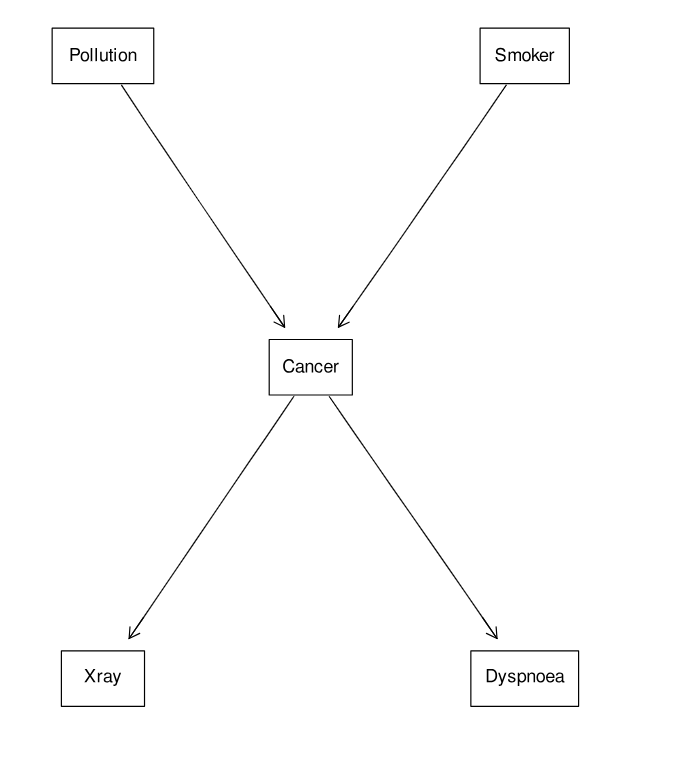
\includegraphics[width=\textwidth]{img/bayesianNetworks/cancerNetwork.png}
        \caption{Red Bayesiana $\childNetwork$ para analizar las enfermedades de niños de recién nacidos. Fuente: \cite{cancerNetwork}}
        \label{fig:cancer_network}
    \end{subfigure}
    \hfill
    \begin{subfigure}[b]{0.6\textwidth}
        \centering
        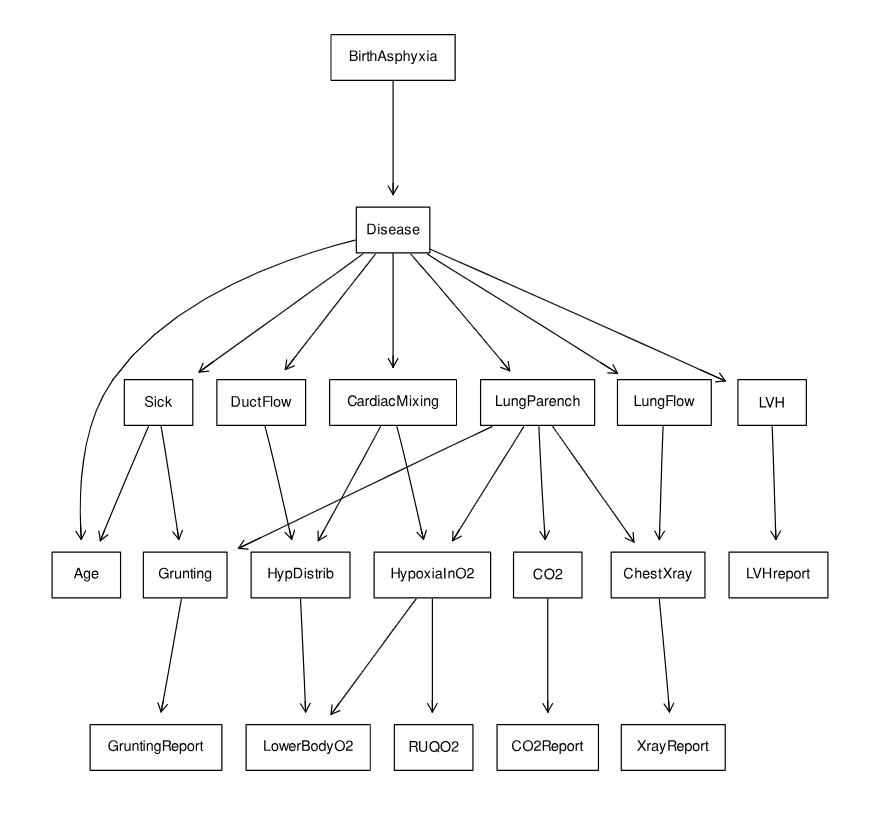
\includegraphics[width=\textwidth]{img/bayesianNetworks/childNetwork.png}
        \caption{Red Bayesiana \cancerNetwork para determinar la probabilidad de tener cáncer de distintos pacientes. Fuente: \cite{childNetwork}}
        \label{fig:child_network}
    \end{subfigure}

    \caption{Ejemplos de redes bayesianas utilizadas en los experimentos.}
    \label{fig:bayesian_networks_combined}
\end{figure}

\paragraph{Especificaciones de los experimentos}

\begin{itemize}
    \item \textbf{Procesador:} Intel(R) Core(TM) i5-7500 CPU @ 3.40GHz
    \item \textbf{Memoria RAM:} 16 GB
    \item \textbf{Sistema operativo:} Ubuntu 22.04 LTS
    \item \textbf{Python:} Versión 3.12
    \item  \textbf{Paquetes:} pgmpy (inferencia bayesiana), sklearn, networkx, shap
\end{itemize}

\subsection{Clases de equivalencia vs Órdenes Topológicos}

Para este experimento, vamos a comparar la implementación clásica de $ASV$ con nuestra idea de utilizar las clases de equivalencia para reducir los términos de la sumatoria. Para eso vamos a comparar la forma original de calcular ASV: 

$$\frac{1}{|topos(G)|} \sum_{\pi \in topos(G)} w(\pi) \left[ \charactheristicFunction(\pi_{<i} \cup {i}) - \charactheristicFunction(\pi_{<i}) \right] $$
con nuestra heurística:
$$\heuristicASVFormula$$

Hay dos métricas a tener en cuenta para ver cuál de estas dos estrategias es mejor. Primero, ver cuánto es el tiempo que se tarda en obtener los conjuntos sobre los que efectuar la sumatoria, que son $eqCl(G, x_i)$ y $topos(G)$. Luego comparar el tamaño de cada uno de esos conjuntos, puesto que por cada elemento de ese conjunto vamos a tener que evaluar a $\charactheristicFunction$ dos veces. Podría ocurrir que la construcción de las clases de equivalencia resulte computacionalmente costosa, y su cardinalidad no necesariamente presente una reducción significativa en comparación con $topos$. En tales casos, el costo adicional de calcularlas puede superar el beneficio esperado, incrementando el tiempo total de cómputo.

\begin{figure}[ht]
    \centering
    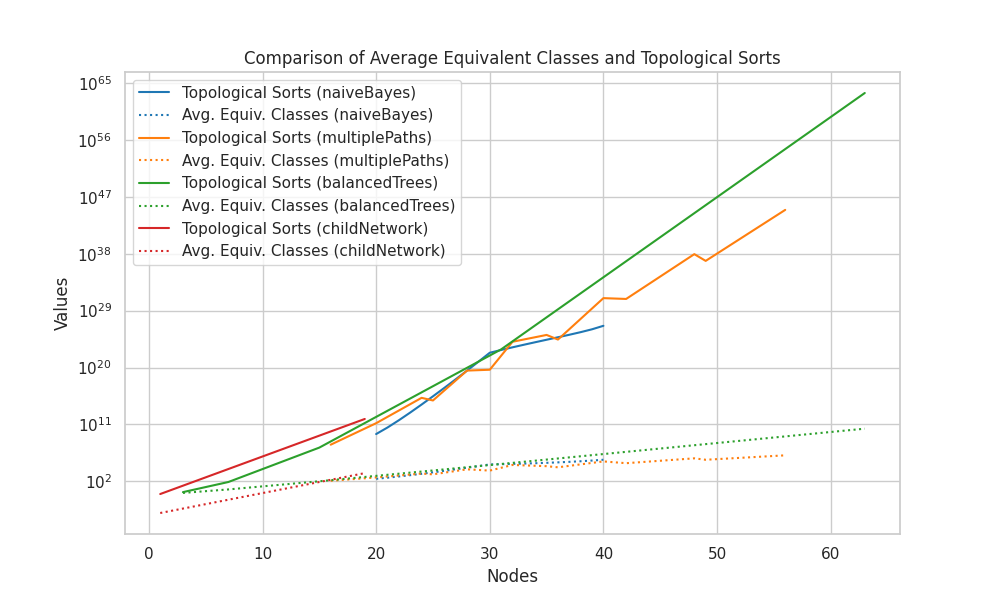
\includegraphics[width=1\linewidth]{img/equivalentClassesVsToposorts.png}
     \caption[Caption for image]{Comparación de clases de equivalencias y órdenes topológicos de distintas clases de grafos. Se utiliza un promedio, puesto que la cantidad de clases de equivalencia depende del nodo que elijamos para calcularlas. \footnotemark }
    \label{fig:equivalenceClassesVsToposortsNumberPlot}
\end{figure}

\footnotetext{La función no es monótona, ya que no se utilizaron todos los grafos posibles para cada una de las clases mencionadas, se realizó una estimación a partir de una muestra significativa de distintos grafos de cada clase. }

%\echu{¿Es mejor tener un gráfico para cada familia? A mi me parecía mejor unificarlos} Queda unificado

Las distintas clases de grafos mencionados en la Figura \ref{fig:equivalenceClassesVsToposortsNumberPlot} son: 
\begin{itemize}
    \item Naive Bayes: Una red Naive Bayes con $n$ nodos, que tiene $n/2$ hojas y que tiene un camino de longitud $n/2-1$ en una de sus hojas. %\santi{No dan las cuentas de la cantidad de nodos} \echu{¿Ahí si, no? Me faltaba la raíz}
    \item Multiple paths: Un bosque compuesto de múltiples caminos de igual longitud. 
    \item Balanced tree: Un árbol binario perfecto balanceado.  
    \item Child network: La red bayesiana \childNetwork, sin algunos de sus ejes para ser un polytree. 
    
\end{itemize}

En la Figura \ref{fig:equivalenceClassesVsToposortsNumberPlot}, podemos observar como el número de clases de equivalencia crece significativamente más lento que el número de órdenes topológicos. Por ejemplo, en el caso de la red $\childNetwork$, la red tiene $7.41\times10^{11}$ órdenes topológicos y 2003 clases de equivalencia en promedio, por lo que si utilizamos las clases disminuimos enormemente la cantidad de llamadas a $\charactheristicFunction$. Luego, para los árboles balanceados, la cantidad de órdenes topológicos es $10^{50}$ veces mayor, una diferencia muy significativa. A partir de estos ejemplos, queda claro que es una mejora hacer el cálculo sobre las clases de equivalencia. Ahora solo queda ver el costo de calcularlas. 

El costo de calcular las clases lo podemos ver en la Figura \ref{fig:equivalenceClassesTimePlot}. Para la mayoría de los grafos de ejemplo que utilizamos tarda menos de 10 segundos. Pero para grafos de mayor tamaño, el tiempo que tarda comienza a crecer exponencialmente, al igual que la cantidad de clases de equivalencia. En el caso puntual de la red \childNetwork tarda menos de 1 segundo en calcular todas sus clases. 


\begin{figure}[ht]
    \centering
    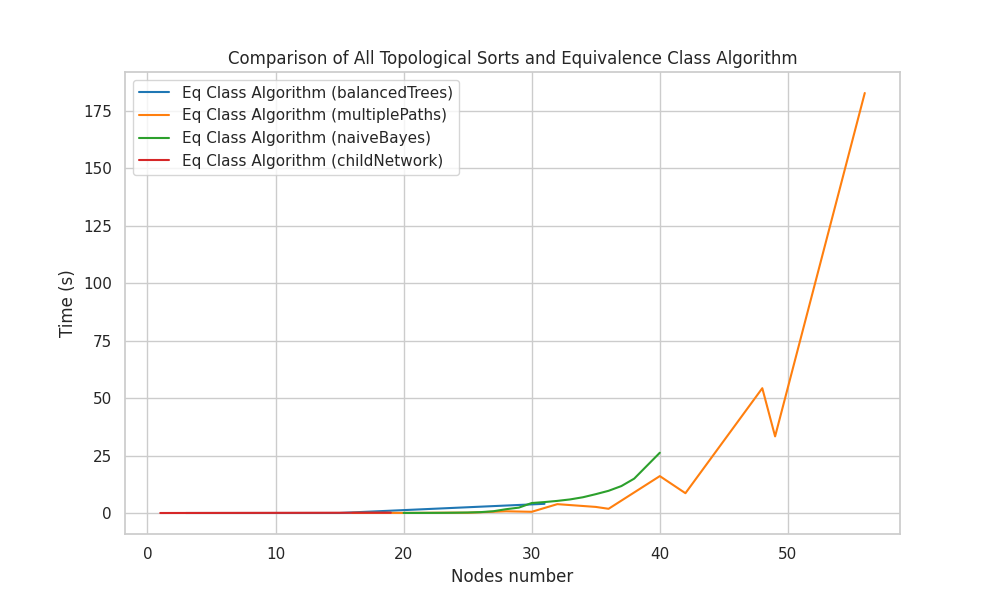
\includegraphics[width=1\linewidth]{img/equivalentClasses_time.png}
    \caption[Caption for image]{Comparación del tiempo que tarda el algoritmo para calcular las clases de equivalencia}
    \label{fig:equivalenceClassesTimePlot}
\end{figure}

\begin{figure}[ht]
    \centering
    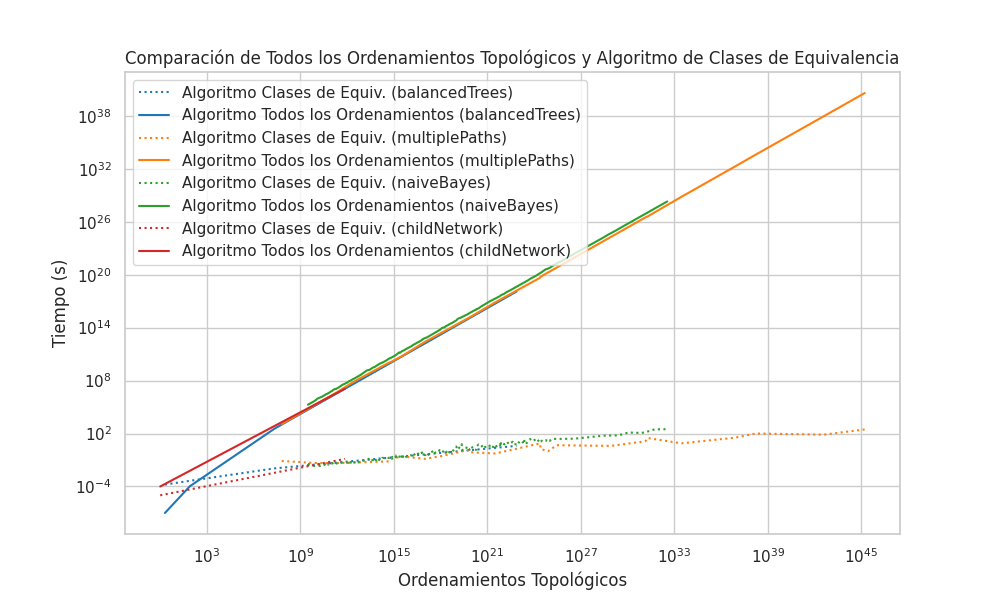
\includegraphics[width=1\linewidth]{img/equivalentClassesVsAllToposorts_time.png}
    \caption[Caption for image]{Comparación del tiempo que tarda el algoritmo para calcular las clases de equivalencia y calcular todos los órdenes topológicos, utilizando una \href{https://networkx.org/documentation/stable/reference/algorithms/generated/networkx.algorithms.dag.all_topological_sorts.html}{implementación} de la librería networkx. \footnotemark }
    \label{fig:equivalenceClassesVsToposortsTimePlot}
\end{figure}


\footnotetext{Para estimar el tiempo que tardaría se calcularon los primeros 1000 órdenes que devuelve el algoritmo exacto. Luego se utilizó ese tiempo para hacer una aproximación del tiempo total, sabiendo la cantidad de órdenes de cada grafo. Esto se realizó por simplicidad, ya que no era viable correr el algoritmo durante tanto tiempo.}

La Figura \ref{fig:equivalenceClassesVsToposortsTimePlot} nos muestra para distintos tipos de grafos cuánto tiempo toma cada algoritmo. En uno se obtienen todas las clases de equivalencia y en el otro todos los órdenes topológicos. A partir de $10^{15}$ órdenes topológicos el problema de calcularlos todos tardaría días, en cambio, calcular las clases de equivalencia sigue siendo una estrategia eficiente. Esto sucede así, puesto que, como vimos en el lema \ref{lemma:upper_bound_equivalence_classes}, la cantidad de clases de equivalencia depende de la estructura del grafo, y no de la cantidad de órdenes.
%\sergio{revisar esta frase, no tiene sentido que solo a partir de $10^{15}$ no es tratable} Rta: Ahí le puse la referencia al gráfico correspondiente y tuvo más sentido, si no era cualquier cosa. 

Por ende, a través de este experimento pudimos ver que la cantidad de clases de equivalencias es significativamente menor que la cantidad de órdenes, por lo que se reduce la cantidad de llamadas a $\charactheristicFunction$. Además, en la figura \ref{fig:equivalenceClassesVsToposortsTimePlot}, podemos ver cómo el tiempo para calcular las clases de equivalencia crece más lentamente que el tiempo de calcular todos los órdenes. Por lo tanto, podemos concluir que el algoritmo proporciona una mejora del tiempo para calcular todas las clases respecto a la implementación naive.
%\echu{Medio raro lo de doblemente efectiva, tal vez habría que expresarlo de otra forma}
%\sergio{Decir algo de que cambia el slope en la escala logarítmica notablemente}

\subsection{ASV vs SHAP}

%\echu{¿Uso emph, bold o alguna otra notación para las redes y las variables?} Sip, emph para redes y texttt para las variables

Este experimento consiste en calcular el valor del $ASV$ y $SHAP$, para cada uno de los features de los modelos utilizados en el experimento de la sección \ref{subSection:experimentoAlgoritmoPromedio}. Vamos a correr este experimento para 5 seeds distintas, ya que los valores obtenidos pueden depender de la aleatoriedad de los datos y queremos contrastar múltiples resultados. Aun así, vamos a elegir una seed para analizar para cada una de las redes, utilizando como criterio para elegir la seed el modelo con la mejor accuracy, ya que si el modelo no aprendió correctamente los patrones subyacentes de los datos, entonces los valores de $ASV$ y $SHAP$ pueden no correlacionarse con el grafo causal original. Los resultados de todas las corridas pueden verse en el apéndice en las Figuras ~\ref{fig:multipleSeedsASVvsShapleyChild} y \ref{fig:multipleSeedsASVvsShapleyCancer}. Correr el $ASV$ para todos los features de la red $\cancerNetwork$ tarda 1 segundo, y correrlo para todos los features de la red $\childNetwork$ tarda 3 minutos. 

Para obtener una intuición acerca de ambas redes y las distintas relaciones entre sus nodos nos basamos en \cite{childNetwork} para la red $\childNetwork$ y \cite{cancerNetwork} para la red $\cancerNetwork$.Además, generamos una Tabla \ref{tab:phi_smoker_with_shift} para ambas redes, para analizar el impacto de modificar cada una de las variables de la red. Por ejemplo, la probabilidad original de la variable \variableNetwork{Smoker} es $P(Smoker=True)=0.3$ pero si sabemos que el paciente tiene cáncer pasa a ser $P(Smoker=True|Cancer=True)=0.8255$. Por lo que (como era de esperarse), \variableNetwork{Cancer} es una variable significativa a la hora de calcular si un paciente es fumador o no. En este caso, vemos que la probabilidad de que sea fumador se vio modificada en 0.5255 al introducir la evidencia de que tenía \variableNetwork{Cancer}. Esta variación de la probabilidad es la que vamos a ver en la columna \emph{Probability Shift} en la Tabla \ref{tab:phi_smoker_with_shift}.

\begin{table}[ht]
    \centering
    \begin{tabular}{|c|c|c|c|}
        \hline
        \textbf{Variable} & \textbf{Smoker} & \textbf{New smoker probability} & \textbf{Probability Shift} \\
        \hline
        \multirow{2}{*}{Pollution = Low} & True  & 0.3 & \multirow{2}{*}{0.0} \\
                                         & False & 0.7 & \\
        \hline
        \multirow{2}{*}{Pollution = High} & True  & 0.3 & \multirow{2}{*}{0.0} \\
                                          & False & 0.7 & \\
        \hline
        \multirow{2}{*}{Cancer = True} & True  & 0.8255 & \multirow{2}{*}{0.5255} \\
                                       & False & 0.1745 & \\
        \hline
        \multirow{2}{*}{Cancer = False} & True  & 0.2938 & \multirow{2}{*}{0.0062} \\
                                        & False & 0.7062 & \\
        \hline
        \multirow{2}{*}{Xray = Positive} & True  & 0.3206 & \multirow{2}{*}{0.0206} \\
                                         & False & 0.6794 & \\
        \hline
        \multirow{2}{*}{Xray = Negative} & True  & 0.2946 & \multirow{2}{*}{0.0054} \\
                                         & False & 0.7054 & \\
        \hline
        \multirow{2}{*}{Dyspnoea = True} & True  & 0.3070 & \multirow{2}{*}{0.0070} \\
                                         & False & 0.6930 & \\
        \hline
        \multirow{2}{*}{Dyspnoea = False} & True  & 0.2969 & \multirow{2}{*}{0.0031} \\
                                          & False & 0.7031 & \\
        \hline
    \end{tabular}
    \caption{Variación de la probabilidad de ser fumador en base a la nueva evidencia}
    \label{tab:phi_smoker_with_shift}
\end{table}

Comencemos analizando el caso de la red $\cancerNetwork$. En la Figura \ref{fig:shapleyVsASVSingleSeedCancer} podemos ver que para $ASV$ la única variable significativa es \variableNetwork{Cancer}. Esto tiene sentido con lo visto en la Figura \ref{fig:cancer_network}, ya que es la única variable conectada directamente con \variableNetwork{Smoker}. Pero si nos basáramos en los resultados obtenidos en los Shapley Values, creeríamos que \variableNetwork{Xray} y \variableNetwork{Dyspnoea} también tienen un impacto significativo en si es fumador o no el paciente. La forma que tenemos para ver cuál de los métodos está detectando correctamente las variables relevantes es la Tabla \ref{tab:phi_smoker_with_shift}, en la cual podemos ver que la variable que más impacta es \variableNetwork{Cancer} y que la \variableNetwork{Dyspnoea} tiene un impacto mucho menor. Esta nueva métrica que vamos a utilizar es igual de arbitraria que Shap, pero nos permitió realizar una comparación y un análisis cuantitativo más allá del significado de cada una de las variables.
%\santi{Nunca definís como se calcula el probability shift}
%\echu{Esto quedo medio raro, lo que quiero decir es que utilizamos esta métrica para que la justificación meramente no sea "Tiene sentido esto, por lo que significan las variables en el mundo real" ¿Se entiende la idea?}.
%\santi{Se entiende, creo.}
Esto ocurre, ya que $ASV$ tiene en cuenta el grafo causal a la hora de realizar estos cálculos, a diferencia de $SHAP$. 

\begin{figure}
    \centering
    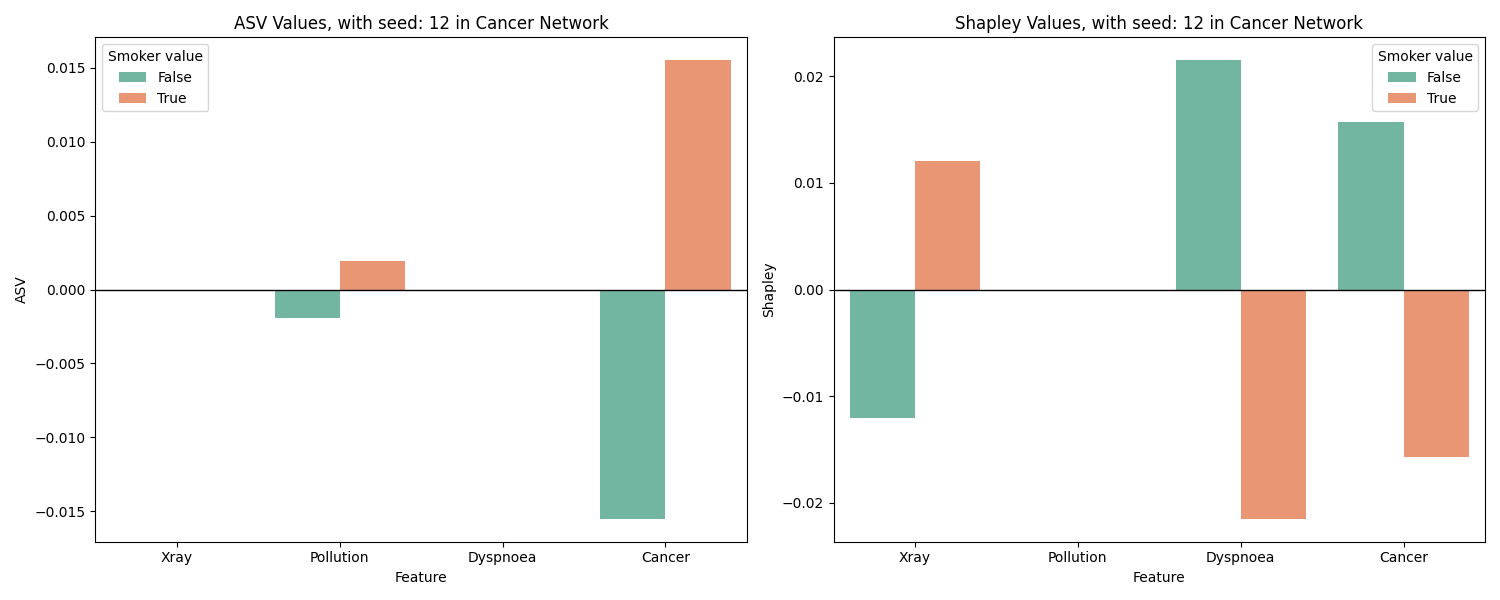
\includegraphics[width=1\linewidth]{img/asvResults/cancerASVAndShapleyExactASVAndShapley.png}
    \caption{Resultados del ASV y Shapley para el modelo con mayor accuracy de los 5 seeds para la red $\cancerNetwork$, con un 81\% de accuracy. }
    \label{fig:shapleyVsASVSingleSeedCancer}
\end{figure}

Luego en el caso de la red $\childNetwork$, estas son las 5 variables más relevantes para las distintas métricas propuestas:

\begin{itemize}
    \item \textbf{Mayor valor de Probability Shift}: Disease, Duct Flow, Sick, Cardiac Mixing, LVH
    \item \textbf{Mayor valor de ASV}: Disease, Duct Flow, Sick, LVH, LVH Report
    \item \textbf{Mayor valor de SHAP}: Disease, ChestXRay, CO2, RUQO2, LVH Report
\end{itemize}

Estos resultados\footnote{Los datos completos se pueden encontrar en \path{\pasantia-BICC\results}, para ver la tabla completa para todas las variables.} se basan en la Figura \ref{fig:shapleyVsASVSingleSeedChild}. Lo que podemos ver es que la intersección entre los features más relevantes de Probability Shift y $ASV$, es mayor a la de $SHAP$ con la misma métrica. Ya que aunque ambos logran identificar a los nodos \variableNetwork{Disease} y a \variableNetwork{LVH/LVH Report} como relevantes, sólo $ASV$ encuentra la relación con \variableNetwork{Sick} y \variableNetwork{DuctFlow}. Aún así esto podría variar según el modelo, ya que si el modelo no logró identificar correctamente las relaciones entre los datos, los valores de $ASV$ y $SHAP$ tampoco van a correlacionarse con el grafo causal. Analizar estos valores nos puede ayudar a ver si tiene sentido la elección de features más relevantes que está utilizando nuestro algoritmo para realizar sus predicciones. 
%\echu{Acá lo polémico es que uso la nueva métrica, Probability Shift, cómo un tipo de ground truth para ver cuáles son los features más relevantes}
%\santi{Si, se ve la complicación. Capaz estaría bueno decir algo más o comparar con otras métricas, pero buneo. Creo igual que el primer ejemplo ya convence de que hay algo raro en SHAP.} Rta: Lo dejamos así también, es lo polémico de usar métricas para comparar. Ninguna es mejor que todas

\begin{figure}
    \centering
    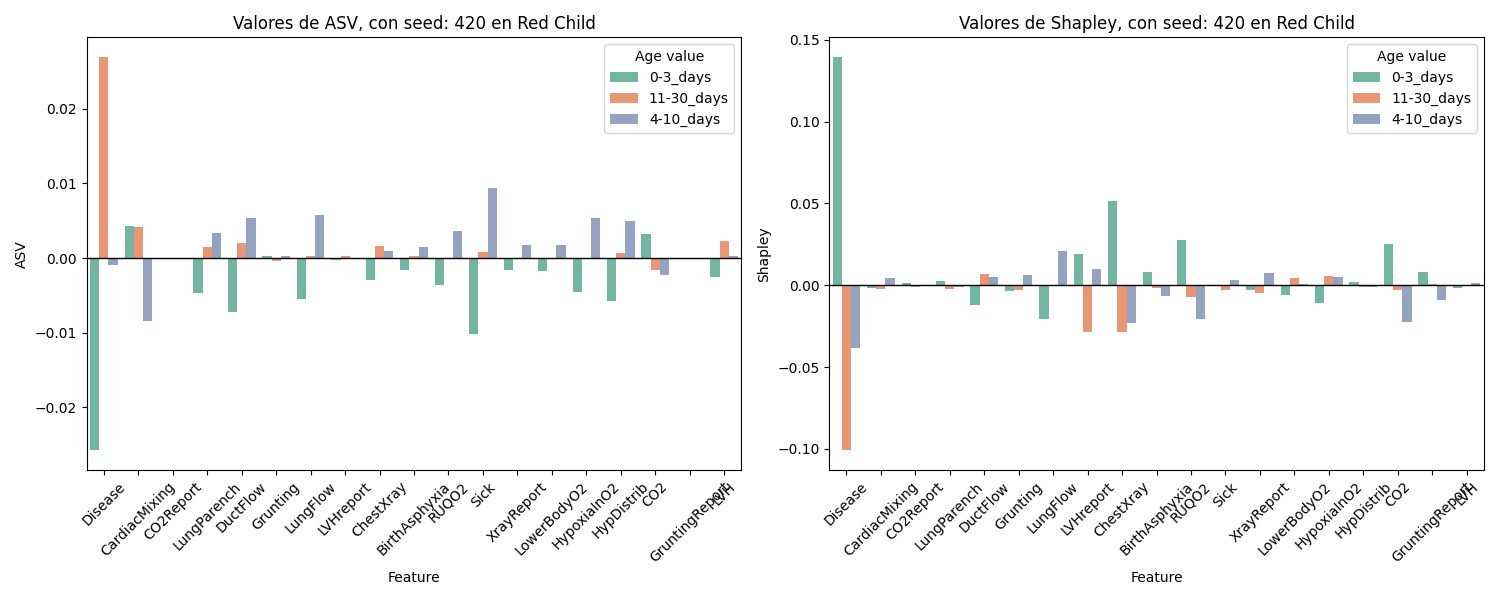
\includegraphics[width=1\linewidth]{img/asvResults/childASVAndShapleyExactASVAndShapley.png}
    \caption{Resultados del ASV y Shapley para el modelo con mayor accuracy de los 5 seeds para la red $\childNetwork$, con un 68\% de accuracy. }
    \label{fig:shapleyVsASVSingleSeedChild}
\end{figure}

En base a lo observado en estos dos casos, podemos ver que $ASV$ puede detectar relaciones entre los features que $SHAP$ no logra encontrar. Esto se debe a que utiliza la información del grafo causal, para ver cuáles features priorizar a la hora de realizar estos cálculos. 

\subsection{ASV exacto sin EqClasses vs ASV aproximado}

El objetivo de este experimento es comparar la performance de obtener los órdenes topológicos de un grafo que es un polytree, pero no es un \dtree. Por lo tanto, solo los podemos obtener sampleándolos con nuestro Algoritmo \ref{alg:topoSortSampling} o generándolos con el algoritmo de Knuth, puesto que las clases de equivalencia solo las podemos obtener para los \dtrees.

\begin{table}[h]
\centering
\begin{tabular}{|l|c|}
\hline
\textbf{Cantidad de órdenes sampleados} & \textbf{Tiempo de sampleo (s)}\\
    \hline
    100 & 0.9270 \\
    1000 & 1.1170 \\
    10000 & 4.7170 \\
    20000 & 7.7170 \\
    30000 & 10.8387 \\
    \hline
    \end{tabular}

\caption{Tiempos de ejecución para muestreo y generación de órdenes topológicos de la red $\childNetwork$}
\label{table:exactVsApproximateTopoSorts}
\end{table}

En la Tabla \ref{table:exactVsApproximateTopoSorts} podemos ver que el enfoque aproximado toma un tiempo tratable para samplear los órdenes. Aunque en nuestro análisis de la complejidad del mismo, habíamos llegado a una cota cuasi polinomial, el algoritmo se comporta de mejor manera en la práctica. También podemos observar que, como se mencionó al introducir el algoritmo de sampleo, su complejidad no es lineal en la cantidad de órdenes sampleados. Esto ocurre, pues vamos obteniendo múltiples candidatos en cada llamado recursivo de la función. 

En base a estos resultados, uno podría creer que la mejor opción es generarlos con el algoritmo de Knuth, el cual tarda menos de 1 segundo en generar los 30000 órdenes. El problema de este algoritmo es que no respeta la distribución de los órdenes.  Por ejemplo, si tuviéramos un grafo como el de la Figura \ref{fig:badExactToposortExample}, podría ocurrir que los primeros 1000 órdenes que nos devuelva el algoritmo tengan como primer nodo a $n_1$. Pero en realidad $n_1$ es el primer nodo en menos del 0.05\% de los casos, por ende no sería una muestra representativa. Para lograr esto deberíamos generar todos los órdenes, pero ya generar meramente un 1\% de los órdenes de la red $\childNetwork$ tomaría más de 2 días. 

%\echu{Este ejemplo, no tan detallado, lo mencionó también en el segundo parrafo de la sección de sampleo. ¿Vale la pena este experimento? Para mi esta bueno para ilustrar porque no garpa usar el algoritmo de Knuth, aunque no sume tantooo}

%\santi{Me parece bien.}

\begin{figure}[ht]
    \centering
    \begin{tikzpicture}
        % Define the rigth set of nodes
        \foreach \i in {1,2,3,4,5}
            \node[draw=none, circle, minimum size=5mm, inner sep=0pt] (L\i) at (4, -\i) {};

        % Define the left set of nodes
        \foreach \j in {1,2,3}
            \node[draw, circle, red, minimum size=5mm, inner sep=0pt] (source\j) at (0, -\j*2) {\scalebox{0.6}{$Source_\j$}};

        % Draw edges between nodes (example edges)
        \foreach \i in {1,2}
            \foreach \j in {1,2}
                \draw[->]  (source\j) -- (L\i); 

        \foreach \i in {4,5}
            \foreach \j in {2,3}
                \draw[->]  (source\j) -- (L\i); 

        \draw[->]  (source2) -- (L3);
        

         \draw [decorate, blue, decoration={random steps, segment length=10pt, amplitude=2pt}, thick]
        (4,-3) circle (2.4);

        %Número de ordenes topológicos para cada nodo

        \node[draw=none,minimum size=3mm, inner sep=0pt] () at (0, -1) {\small \textcolor{orange}{$n_1$=1000}};

        \node[draw=none,minimum size=3mm, inner sep=0pt] () at (0, -3) {\small \textcolor{orange}{$n_2$=100000}};

        \node[draw=none,minimum size=3mm, inner sep=0pt] () at (0, -5) {\small \textcolor{orange}{$n_3$=100000}};
    \end{tikzpicture}
    \caption{Posible comienzo del algoritmo exacto, con los candidatos a ser el primer nodo del orden en rojo y el resto del grafo en azul. Cada node fuente (source) tiene sus respectivas cantidades de órdenes topológicos en los que está primero.}
    \label{fig:badExactToposortExample}
\end{figure}

Por último, realizamos un experimento para calcular el error al calcular $ASV$ con el método aproximado, sampleando 1000 órdenes topológicos de la red $\childNetwork$. En la Figura \ref{fig:boxplotASVApproximateDifferences} podemos ver los resultados de esta corrida. La mayoría de los valores aproximados obtenidos tiene un error del 8\% con respecto a su valor exacto. Las diferencias más altas se corresponden a valores de $ASV$ muy pequeños, como 0.005, por lo que una pequeña diferencia en su valor calculado relativamente es más significativa. Esto es esperable, ya que el error mencionado en el Teorema \ref{theorem:asvSamplingError} es un error absoluto, no relativo. Para los features con valores mayores a 0.01, su diferencia es menor al 5\%.
%\santi{Esto es esperable: nuestro teorema habla de error absoluto, no del relativo. Podrías decirlo.}
Con estos resultados, podemos concluir que no es necesario obtener todos los ordenes y con una buena aproximación podemos obtener resultados medianamente precisos. 


\begin{figure}
    \centering
    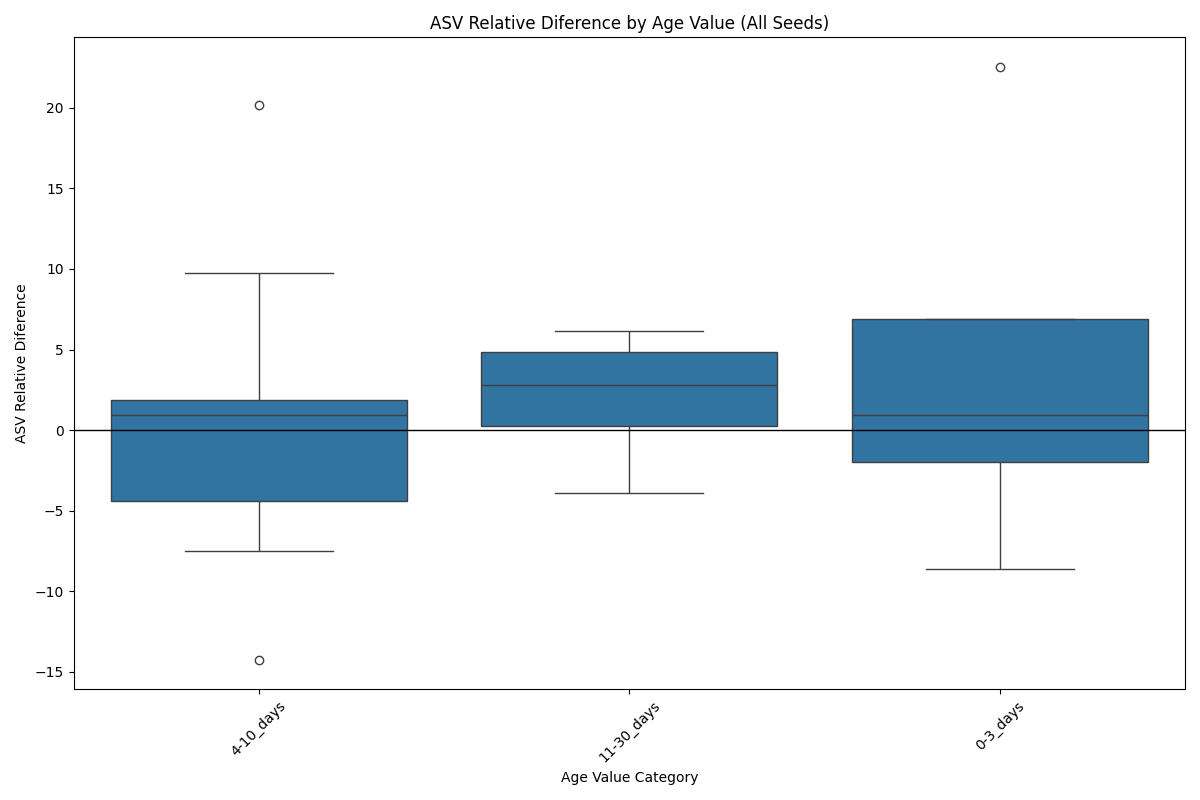
\includegraphics[width=0.8\linewidth]{img/asvResults/ChildAllSeedsASVBoxplot.png}
    \caption{Diferencia relativa entre los valores del ASV aproximado y el exacto para la red $\childNetwork$, se utilizaron las diferencias de cada una de las 5 seeds.}
    \label{fig:boxplotASVApproximateDifferences}
\end{figure}

% \echu{¿Tiene sentido hacer un experimento en el cuál comparo para distintos grafos, los árboles por ejemplo, cuán cercana es la distribución original a la sampleada? Puedo samplear y ver como me quedan distribuidas las clases de equivalencia. Intentando hacer algún calcúlo para ver cuán cercanas son esas clases de equivalencia a las originales. Respuesta de Santi: Noup, es justamente lo que hace el algoritmo, buscar samplear de las clases de equivalencia}

\subsection{Algoritmo de promedio para DT binarios}
\label{subSection:experimentoAlgoritmoPromedio}
Para este experimento vamos a comparar la forma naive de obtener la predicción promedio para una permutación y el algoritmo \ref{alg:meanPredBinDT}, que utiliza la estructura del árbol para calcularlo con complejidad $O(i|V| + (varElim)l)$. La idea es comparar el tiempo que tardan ambos algoritmos y ver cómo se asemejan estos promedios a las probabilidades originales de la red. Dentro del cálculo de $\assym(x,i)$, para la instancia $x$ y el feature $i$, lo que queremos calcular es:
$$\charactheristicFunction(\toOr) = \mathbb{E}_{\aBayesianNetwork(x' | x)}[f_y(x_{\toOr \leq i} \cup x'_{\toOr > i})]$$

%\echu{La segunda es la fórmula que utilizo en la sección 2 para introducir al promedio, pero me gusta más la que utilizo acá porque siento que se entiende más para explicar la idea. ¿Puedo decir que ambas significan lo mismo y explicar porque? Además a M le falta el $_y$, aunque podría usar $M_y$ en vez de $f_y$ tal vez.}

A través de una permutación $\toOr$ de los features de $x$ definimos qué features quedan fijos y cuáles varían. La función de probabilidad que se utiliza es $\aBayesianNetwork(x' | x)$, la cual utilizamos para calcular la probabilidad de los valores de $x'$ dados los valores de $x$. Esta predicción promedio la vamos a calcular para cada uno de los posibles valores\footnote{Recordemos que podemos tener variables no binarias, por lo que $y$ puede tomar más valores que 0 o 1.} $y$ de $p$, el feature a predecir. $f_y(x)$ es un clasificador binario que devuelve $1$ si nuestro árbol de decisión le asigna la clase $y$ a la instancia $x$ y $0$ en el caso contrario. A continuación presentamos la implementación naive para calcular $\charactheristicFunction$. 
%\santi{El $y$ es el resultado entonces? ¿No alcanza entonces con poner $f_1()?$} Rta: No se había entendido que era para variables no binarias
%\echu{No entendí, $y$ es la clase que queres clasificar. Cómo no necesariamente son binarios los párametros entonces puede tomar todos los valores del dominio de la variable a predecir} 

Para calcular $\mathbb{E}_{\aBayesianNetwork(x' | x)}[f_y(x_{\toOr \leq i} \cup x'_{\toOr > i})]$ lo que vamos a hacer es generar todas las instancias $x_{prom} \in (x_{\toOr \leq i} \cup x'_{\toOr > i})$, en las cuales los valores de los features que aparece luego de $x_i$ en $\toOr$ van a ser variables, y el resto van a ser fijos. Por fijos nos referimos a que van a tener los mismos valores que $x$, y sus otros features van a tomar todos los valores posibles. A partir de estas instancias vamos a calcular la función característica\footnote{La notación para la función característica es distinta a la utilizada al introducirla en la fórmula \ref{formula:characteristicFunctionDefinition}, pero su significado es el mismo. En este caso $(x_{\toOr \leq i} \cup x'_{\toOr > i})$ son nuestras instancias consistentes y $f_y$ es nuestro clasificador binario $M$. Para cada valor de $y$, $f_y$ devuelve 1 si la etiqueta clasificada es $y$ y 0 en el caso contrario.} cómo:

$$\charactheristicFunction(\toOr) = \sum_{x_{prom} \in (x_{\toOr \leq i} \cup x'_{\toOr > i})} p_\aBayesianNetwork(x_{prom} | x) f_y(x_{prom}) $$

%\santi{¿Para cuál valor de $y$?}
%\echu{Para cada valor de $y$ tenes una nueva función, lo aclare en el footnote. }

Por lo tanto, para esta cuenta vamos a necesitar generar todas las instancias $(x_{\toOr \leq i} \cup x'_{\toOr > i})$, y luego evaluar nuestro árbol de decisión $DT$ y a la red bayesiana $\aBayesianNetwork$ para cada una de estas instancias. Evaluar él $DT$ cuesta $O(d)$, siendo $d$ la profundidad del $DT$. Si tomamos a $c$ como la cardinalidad máxima de un feature y a $vars$ como el tamaño del conjunto de features variables, la complejidad temporal de la implementación naive es $O(vars^c(varElim + d)$, siendo $O(vars^c)$ la cantidad de instancias generadas. 

Así las complejidades que nos quedan son $O(vars^c(varElim + d))$ y $O(i|V| + (varElim)l)$, para cada uno de nuestros algoritmos. Podemos ver que la solución naive depende de la cantidad de features variables del $\toOr$, a diferencia del otro algoritmo, que corre el promedio directamente sobre la estructura del $DT$.

%\santi{$v$ no debería ser $|V|$? } Rta: Sip

%\echu{¿Tiene sentido lo de poner el valor que da la predicción del feature? Para mi un poco si para explicar que tipo de feature es y porque da esos valores. } Rta: Sip, tiene sentido

\begin{figure}[ht]
    \centering
    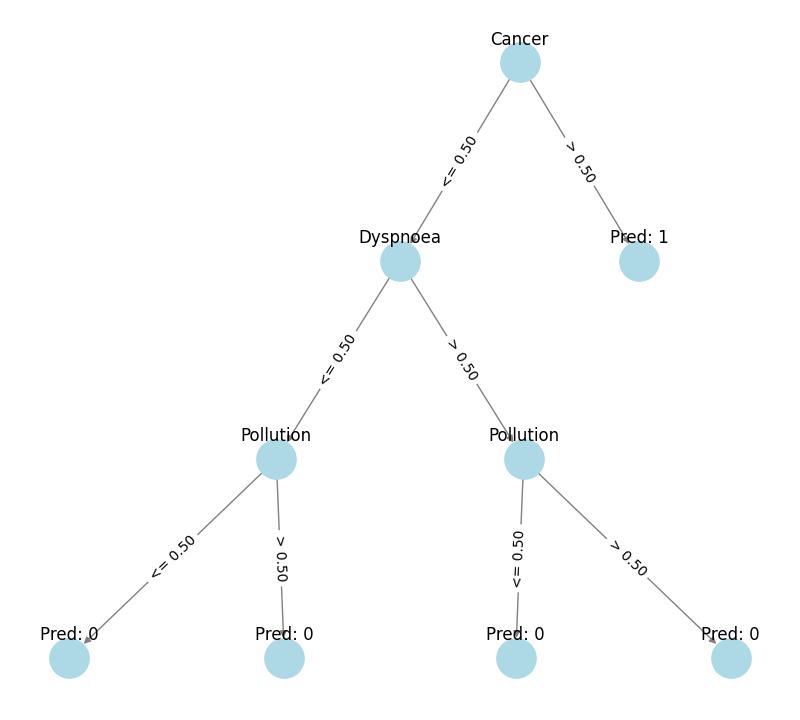
\includegraphics[width=0.7\linewidth]{img/cancerDecisionTree.png}
    \caption{Árbol de decisión generado a partir de los datos de la red $\cancerNetwork$. Las hojas contienen el valor de la predicción que devuelve el modelo (0 o 1)}
    \label{fig:cancerDecisionTree}
\end{figure}

Para la red $\cancerNetwork$ se generaron 600 instancias con un árbol de decisión de altura 3 y para la red $\childNetwork$ se generaron 10000 instancias con un árbol de decisión de altura 9. Las probabilidades de la red bayesiana son los valores que devuelve la consulta $P(X = z)$ para la red $\aBayesianNetwork$ y los distintos valores $z$ de cada feature $X$. El método \emph{Algoritmo promedio (probabilidades)} consiste de la predicción promedio, si en el árbol en vez de devolver una predicción de 1 o 0 se devolviera una probabilidad en las hojas. Este método es distinto al algoritmo evaluado en esta tesis, pero nos pareció interesante agregarlo para analizar la diferencia entre los promedios al usar una predicción probabilística. 
%\santi{Medio feo usar $y$ para dos cosas distintas.} Rta: Concuerdo

\begin{table}[ht]
    \centering
    \begin{tabular}{l c c}
        \toprule
        \textbf{M\'etodo} & \textbf{Predicci\'on} & \textbf{Tiempo (segundos)} \\
        \midrule
        Algoritmo promedio & [0.98255, 0.01745] & 0.0165 \\
        Algoritmo promedio (probabilidades) & [0.7213, 0.2787] & 0.0043 \\
        Implementaci\'on naive & [0.98255, 0.01745] & 0.0043 \\
        Probabilidades red bayesiana & [0.7, 0.3] & - \\
        \bottomrule
    \end{tabular}
    \caption{Valor promedio de la predicci\'on del feature \textbf{Smoker} en la red bayesiana $\cancerNetwork$, dejando variables todos los features}
    \label{table:cancerMeanResults}
\end{table}
%\sergio{Cuidado con la coherencia de CANCER, cancer, \it{cancer}} 

\begin{table}[ht]
    \centering
    \begin{tabular}{l c c}
        \toprule
        \textbf{M\'etodo} & \textbf{Predicci\'on} & \textbf{Tiempo (segundos)} \\
        \midrule
        Algoritmo promedio & [0.9916, 0.0, 0.0084] & 0.0258 \\
        Algoritmo promedio (probabilidades) & [0.7577, 0.0746, 0.1677] & 0.0258 \\
        Implementaci\'on naive & [0.9916, 0.0, 0.0084] & 19.6774 \\
        Probabilidades red bayesiana & [0.6490, 0.1715, 0.1795] & - \\
        \bottomrule
    \end{tabular}
    \caption{Valor promedio de la predicci\'on del feature \textbf{Age} en la red bayesiana $\childNetwork$, dejando variables 11 de los 20 features y utilizando a $x\in data$ t.q $f(x)=0$.}
    \label{table:childMeanResults}
\end{table}

Al analizar la Tabla \ref{table:cancerMeanResults} podemos ver que en ambos casos se tiende a sobrerrepresentar una clase. Esto ocurre ya que el modelo entrenado predice 0 para la mayoría de los inputs y la probabilidad de los inputs para los cuales predice 1 es más baja. En la Tabla \ref{table:childMeanResults} ocurre lo mismo respecto a la sobrerrepresentación. Por lo que, en realidad, la predicción promedio solo va a ser tan buena como el modelo que haya sido entrenado. Esto no depende del algoritmo, sino del entrenamiento del modelo.
Además, podemos ver que la implementación naive es más lenta. Esto se debe a que la mediana de la cardinalidad de cada feature es 3. Por lo que cada feature agregado va a hacer que se tarde 3 veces más en promedio. Para órdenes topológicos que dejaran los 19 features variables la implementación naive tardaría \textbf{más de 1 día}. En cambio, la performance del algoritmo promedio no se ve tan afectada por la cantidad de features variables, sino que depende del tamaño del árbol de decisión. Finalmente, se destaca que las predicciones más cercanas a las probabilidades generadas por la red bayesiana son aquellas que utilizan directamente las probabilidades como output, en lugar de predicciones binarias (0/1). Esto se debe a que estas predicciones son más granulares y, por ende, reflejan con mayor fidelidad las distribuciones probabilísticas subyacentes. Podemos ver en la Figura~\ref{fig:cancerDecisionTree} que el patrón aprendido por el árbol es muy simple $f(x) = $ \textbf{If} $x_{cancer} > 0.5$, \textbf{then} 1, \textbf{else} 0. Luego como $P(Cancer = 1) = 0.01745$, el valor del promedio que vemos en la Tabla \ref{table:cancerMeanResults} va a representar esa predicción. 

Se puede contemplar que los valores de la implementación naive y del algoritmo promedio son idénticos, puesto que ambos están calculando lo mismo. Solo que mientras nuestro algoritmo calcula la probabilidad de llegar a una hoja, la implementación naive genera todas las instancias que pueden llegar a la misma, para luego clasificarlas y calcular su probabilidad. Así que teniendo en cuenta que ambos calculan el mismo valor, podemos concluir que el algoritmo introducido ofrece una mejora significativa respecto a la implementación naive. 
%Esto ocurre ya que el algoritmo del promedio en $DT$ utiliza las hojas del $DT$ para realizar su cálculo, en cambio, la implementación naive genera instancias nuevas a partir de los features variables. Por lo que no necesariamente van a tener el mismo valor estos dos algoritmos, aun así su diferencia no va a ser significativa. Esto puede significar un problema para nuestro algoritmo si resulta que el árbol de decisión no tiene instancias representativas en sus hojas, ya que el valor del promedio no va a tener en cuenta a una muestra significativa. 
%\sergio{Revisar, repensar, repent. No deberia dar distinto, revisar el caso en el cual da y evaluar porque. Si es que no es un bug y tiene sentido, meteer una oraci[on que lo explique mejor. } RTA: Había flasheado, al final si eran iguales
%\santi{Adem[as en la seccion hablas del valor de la prediccion ylos comparas. Cuando en la intro solo hablas del tiempo, aclarar que se va a tener eso en cuenta tambi[en. Si no lo vas a hacer, remover el valor de las tablas.}


%\santi{Mover esta primer expeimentación al final, es la menos importante.}

%\sergio{recordar de unificar capitalización Tablas, Sección, Figura, etc.}

\section{Conclusión}\label{Section:Conclusion}

\begin{frame}{Conclusiones}
	\dificultyLevel{1}
	\begin{itemize}[<+- | alert@+>]
		\item Se optimiz\'o el c\'alculo de ASV en datos con distribuciones bayesianas y árboles de decisión.
		\item Se demostr\'o la tratabilidad para Naive Bayes.
		\item Se desarroll\'o un algoritmo exacto eficiente para la predicci\'on promedio en árboles de decisión.
		\item Se defini\'o una heur\'istica basada en clases de equivalencia para reducir las evaluaciones.
		\item Se construy\'o un algoritmo de sampleo de órdenes topológicos con performance tratable en grafos con grados acotados.
		%\item En la pr\'actica: la heur\'istica reduce llamadas a $\charactheristicFunction$, aunque requiere optimizaci\'on.
	\end{itemize}
\end{frame}

\begin{frame}{Conclusiones}
	\dificultyLevel{1}
	\begin{itemize}[<+- | alert@+>]
		\item Se implement\'o una versi\'on exacta y otra aproximada para ASV.
		\item Se comprobó empiricamente que las clases de equivalencia proporcionan una mejora significativa. 
		\item El principal aporte es la optimizaci\'on de ASV mediante clases de equivalencia respecto de los órdenes topológicos.
	\end{itemize}
\end{frame}

\begin{frame}{Trabajo Futuro}
	\dificultyLevel{1}
	\begin{itemize}[<+- | alert@+>]
		\item Generalizar algoritmo de clases de equivalencia a \emph{polytrees}.
		%\item Optimizar el algoritmo de conteo de órdenes topológicos.
		\item Implementar nuevas estrategias de sampleo y conteo. % \cite{HUBER2006420, efficientCountingOfToposorts}.
		\item Extender la implementación de ASV para modelos y distribuciones arbitrarios.
		\item Estudiar propiedades de complejidad del sampleo y conteo de órdenes tópologicos.
		\item Explorar algoritmos alternativos para enumerar órdenes tópologicos.
		
	\end{itemize}
\end{frame}



%%%% BIBLIOGRAFIA
\bibliography{biblio}{}
\bibliographystyle{plain}

\section{Apéndice}\label{Section:Apendice}

\begin{comment}
    %Con muchisimo dolor, esto se queda afuera de la tesis

    \subsection{Variable Elimination} \label{subSection:variableEliminationAlgorithm}

A continuación vamos a ver una explicación un poco más detallada del algoritmo \emph{Variable Elimination}. La operación de inferencia que queremos realizar con el mismo es $P(X_q \mid X_{e_1} = v_1 \land \ldots \land X_{e_j} = v_j)$, siendo $X_{e_1} = v_1 \land \ldots \land X_{e_j} = v_j$ la evidencia introducida en la red y las $X_{o_i} \neq X_q$ con $o_i \neq e_k$ nuestras variables ocultas. Primero descomponemos esta query en una sumatoria y multiplicación de probabilidades condicionales, basándonos en las dependencias de nuestra red bayesiana. Una vez que tenemos una sumatoria del estilo $\sum_{X_{h_1}} \ldots \sum_{X_{h_j}} P(..| ..) \ldots P(..| ..)$ nuestro algoritmo consiste en:  

\begin{enumerate} \label{alg:variableElimination}
    \item \textbf{Construir} un factor para cada distribución de probabilidad condicional.
    \item \textbf{Restringir} las variables observadas a sus valores observados.
    \item \textbf{Eliminar} cada variable oculta $X_o$:
    \begin{itemize}
        \item \textbf{Multiplicar} todos los factores que contienen $X_o$ para obtener un nuevo factor $g_j$.
        \item \textbf{Sacar} la variable $X_o$ del factor $g_j$ mediante suma.
    \end{itemize}
    \item \textbf{Multiplicar} los factores restantes.
    \item \textbf{Normalizar} el factor resultante, para que las probabilidades sumen 1.
\end{enumerate}

\santi{Estos itemizes generan un monton de duda ¿Qué es un factor? ¿Cómo es lo de eliminar una variable oculta?}

Su complejidad es polinomial basándose en la cantidad de variables y exponencial en base al tamaño de su mayor factor (siendo el tamaño la cantidad de variables del mismo). No podemos hacer algo mejor que la exponencial en el tamaño, pues el tamaño de una CPT de una variable de la red bayesiana $\aBayesianNetwork$ está dado por $O(c^f)$, siendo $c$ la cardinalidad máxima de una variable y $f$ la cantidad de variables en el factor. Por lo tanto, en principio $VE$ sería polinomial en el tamaño de $\aBayesianNetwork$, puesto que las operaciones de construir, restringir, multiplicar, remover y normalizar son polinomiales en base al tamaño. Dado que además la cantidad de nuevos factores que vamos a introducir son $O(n)$, con $n$ la cantidad de variables de $\aBayesianNetwork$.

%\santi{El tamaño no es en realidad $O(\sum_{v \in N} c_v^{f_v})$ donde $c_v$ es la cardinalidad del nodo $v$ y $f$ su cantidad de padres?} Echu: Noup, porque acá estoy hablando de una CPT individual de una variable, esa cota sería para todas las CPT's. Reformule la oración porque no se entendía eso. 

Pero tenemos un problema, en el tercer paso al eliminar la variable oculta $X_o$ puede ser que el nuevo factor $g_j$ sea mayor que todos los factores originales de $\aBayesianNetwork$, en ese caso la complejidad puede no ser polinomial. Al tamaño máximo de los nuevos factores $g_j$ se le llama ancho de eliminación (\emph{elimination width}). Esta medida se relaciona con el \emph{tree width}, puesto que el mejor \emph{elimination width} que uno puede obtener para los $n!$ órdenes posibles de eliminación de $\aBayesianNetwork$ es el \emph{tree width}. A raíz de esto es que se define la complejidad de este algoritmo como exponencial en el \emph{tree width} de $\aBayesianNetwork$, siendo esta $O(n*c^{ew})$, con $n$ la cantidad de variables, $c$ la cardinalidad máxima de una variable y $ew$ el ancho de eliminación. 

Igualmente, un valor acotado de $ew$ no alcanza, ya que encontrar el orden óptimo de eliminación es un problema \NP{-hard} \cite{orderingNpHard}, por lo que podría ser que encontrar este orden tampoco sea posible en tiempo polinomial. 

La complejidad de este algoritmo fue estudiada en varios artículos, por ejemplo en \cite{peyrard2018exactapproximateinferencegraphical} muestran distintos tipos de grafos en los cuáles \emph{Variable Elimination} (VE) puede realizarse en tiempo polinomial. Los \emph{polytrees} son uno de estos casos, ya que el orden de eliminación óptimo se puede encontrar en tiempo polinomial, el cuál corresponde al inverso del orden topológico. Puesto que en cada paso de la eliminación la cantidad de vecinos de ese nodo va a ser 1, por lo que su \emph{elimination width} va a ser 1, y por lo tanto la ejecución del algoritmo va a tardar un tiempo polinomial en el tamaño de la red. Por lo que la familia de grafos 
 %Ver si tiene sentido poner las explicaciones, ejemplos y dibujos del paper peyrard2018exactapproximateinferencegraphical, que la verdad están muy buenas. 
 %RTA Cifu: Ya está quedando muy larga, no agreguemos cosas que no suman tanto. 

\end{comment}
 

\subsection{Fórmulas }

\subsubsection{Funciones auxiliares del cálculo de los unrelated trees} \label{subsubSection:auxiliaryFormulasUnrelatedTrees}

Está es la definición de la función \textit{union} utilizada en la Ecuación \ref{formula:unrelated_equiv_classes}:

\begin{align}\label{formula:union}
&\union(((repEC_1, lTopo_1, rTopo_1), ...., (repEC_{|n|}, lTopo_{|n|}, rTopo_{|n|})), n_t) = \nonumber \\ 
&\left(\bigcup_{j=1}^{|n|} repEC_j \cup \set{n_t}, \binom{\sum_{i=1}^{|n|} L(repEC_i)}{L(repEC_1), \ldots, L(repEC_{|n|})} \prod_{i=1}^{|n|} lTopo_i, 
\binom{\sum_{i=1}^{|n|} R(repEC_i)}{R(repEC_1), \ldots, R(repEC_{|n|})} \prod_{i=1}^{|n|} rTopo_i \right)
\end{align}

La función $\union$ está definida en la Ecuación~\ref{formula:union}, y es la encargada de unir las distintas clases de equivalencia de los hijos de un nodo $n$. Más formalmente, $\union(n, ((repEC_1, lTopo_1, rTopo_1), \ldots)$ es la clase de equivalencia que se representa con $repEC$ en la cual el nodo $n$ está a la izquierda de $x_i$ y es compatible con las clases $repEC_i$ (en el sentido de que si un nodo aparece a la izquierda en $repEC_i$ entonces este también aparece a la izquierda en $repEC$, y de la misma forma con los que aparecen a la derecha). Para calcular la cantidad de órdenes topológicos a la izquierda y a la derecha de la clase utilizamos una fórmula muy similar a \ref{for:topoCountingDTrees}. Se puede aplicar la misma lógica porque no hay dependencias entre los nodos de los árboles no relacionados y sus subárboles, por lo que podemos combinar los órdenes topológicos sin restricciones.

\paragraph{Complejidad temporal de $union$}

$\union$ realiza 4 operaciones de costo $O(n)$ (pues $d_{out}(node)<n)$, 2 $\prod \ y \ \sum$. El coeficiente multinomial\footnote{Utilizamos el modelo de 
memoria RAM teniendo en cuenta que los factoriales pueden estar precalculados y que multiplicar números es $O(1)$ más allá de su tamaño. Igualmente si el multinomial tomara $O(n^2)$, la complejidad total seguiría siendo la misma.} tiene costo $O(n)$, por lo que $\union$ tendrá una complejidad temporal de $O(n)$



\subsubsection{Función completa de \leftPossibleOrders} \label{subsubSection:leftOrdersImplementation}

A continuación vamos a ver la implementación del algoritmo descrito en la sección \ref{alg:leftOrdersAlgorithm}. Los parámetros de la función serán:
\begin{itemize}
    \item $p$: posición en la que se colocó el último ancestro.
    \item $i$: índice del ancestro que vamos a colocar.
    \item $nodesPerAncestor$: una lista que tiene, en la posición $i$-ésima, el número de nodos a la izquierda del unrelated tree de $a_i$.
        \begin{itemize}
            \item Debido a la ligera mejora mencionada en la sección \ref{slight_improvement}, solo habrá un árbol debajo de cada $a_i$, ya que si hay más de uno, estos árboles serán fusionados en uno solo. 
        \end{itemize}
\end{itemize}

Estas son las funciones auxiliares que vamos a utilizar:
\begin{itemize}
    \item $\mathrm{possibleCombinations}(l,i,nodesPerAncestor) \ \text{o} \ pb$, que devuelve todas las formas posibles de sumar los primeros $i$ elementos de $nodesPerAncestor$ para obtener $l$.
        \begin{itemize}
            \item Por ejemplo, $\mathrm{possibleCombinations}(5,3,[4,2,1,7,\dots])= [[4,0,1], [4,1], [3,1,1], [3,2], [2,2,1]]$.
        \end{itemize}
    \item $\mathrm{hasPlaced}(placedNodes, nodesPerAncestor) \ \text{o} \ hp$, devuelve una lista $l$ que tiene en la posición $i$-ésima el elemento $l[i]= nodesPerAncestor[i] - placedNodes[i]$. Lo que hace es restar de $nodesPerAncestor$ los elementos que ya colocamos en $placedNodes$.
    \item $\mathrm{canPlace}(i ,nodesPerAncestor) \ \text{o} \ cp$, devuelve la suma de los primeros $i$ elementos de $nodesPerAncestor$.
\end{itemize}
Teniendo en cuenta estas función, la fórmula\footnote{Pueden encontrar este algoritmo en \path{\pasantia-BICC\asvFormula\classesSizes\recursiveFormula.py}} que vamos a utilizar para calcular los posibles ordenamientos de los nodos de las distintas clases de equivalencia de cada subárbol es:

%\label{formula:left_possible_orders}

 \[
    \leftPossibleOrders(p,i,npa) = 
    \begin{cases} 
    \begin{aligned}
        \binom{ cp(i, npa)}{npa[1], \ldots, npa[i]} 
    \end{aligned} & \text{if $|A|=i$} \\
    \begin{aligned}
    &\sum_{toFill=p}^{p+cp(i,npa)} \sum_{comb \in pb(toFill-p-1,i, npa)} \Big(\binom{ sum(comb)}{comb_1, \ldots, comb_i} \\
    &  * \leftPossibleOrders(toFill,i+1,hp(comb, npa)\Big)
    \end{aligned}
    & \text{otherwise}
    \end{cases}
\]

%\echu{ Esto en realidad es más complejo, hay algunas transformaciones que se tienen que hacer a left. ¿Las anoto o no tiene sentido? (Es lo que se hace en leftElementsOfClasses en el código)} Rta: No hace falta, ya es suficientemente compleja la explicación y esa información no suma a entender el algoritmo

Nuestro caso base es cuándo ya hemos colocado todos los ancestros, por lo que sólo queda combinar los nodos que nos quedan por colocar. Luego en el caso recursivo, el $toFill-p-1$ es el número de posiciones que necesitamos llenar entre el $a_i$ que estamos colocando y el $a_{i-1}$ que se colocó antes. En cada paso realizamos la sumatoria de, cada posible combinación, $comb$, de los elementos de $npa$, teniendo en cuenta todas las posibilidades de la cantidad de posiciones a llenar $toFill$ entre $a_i$ y $a_{i-1}$, las posiciones van desde $p$ hasta $p$ más la máxima cantidad de nodos que podemos colocar ($cp(i,npa)$). 
Ahora, con todas estas funciones definidas, la llamada que resolverá $leftOrders(A, left)$ será $\leftPossibleOrders(0,0,left)$.

Para entender un poco como funciona este algoritmo veamos cuál podría ser un paso del mismo. En la Figura \ref{fig:leftOrdersIterationTopoOrder} podemos ver como sería el estado actual de los órdenes topológicos que estamos contando, teniendo en cuenta las decisiones previas que tomamos. Los nodos pintados en naranja que vemos en la Figura \ref{fig:leftOrdersIterationGraph} son los nodos que tenemos disponibles para rellenar ese espacio en rojo. En cambio los nodos de $u_i$ no los podemos utilizar todavía, ya que todavía no colocamos el nodo $a_i$, una vez que lo coloquemos podremos utilizarlos. 

%\echu{ Hace falta agregar un dibujo o ilustración para que el algoritmo quede más claro?}
%\%sergio{Creo que vendría muy bien}

\begin{figure}[ht]
    \centering
    \begin{tikzpicture}
        % Línea principal
        \draw[thick] (0,0) -- (10,0);

        % Segmento azul: inicio -> a_{i-1}
        \draw[blue, very thick] (0,0) -- (4,0);

        % Segmento rojo: a_{i-1} -> a_i
        \draw[red,  very thick] (4,0) -- (6,0);
        
        % Marcas y etiquetas
        \foreach \x/\etiqueta in {2/$a_1$, 4/$a_{i-1}$, 6/$a_i$, 8/$a_{|A|}$} {
            \draw (\x,0.2) -- (\x,-0.2);          % ticks
            \node[below] at (\x,-0.2) {\etiqueta}; % etiquetas
        }

        % Puntos suspensivos
        \node at (1,0.2) {$\cdots$};
        \node at (5,0.2) {$\cdots$};
        \node at (9,0.2) {$\cdots$};
    \end{tikzpicture}
    \caption{$i$-ésimo paso de \leftPossibleOrders, la línea azul son son los nodos ya colocados y la línea roja tiene longitud $toFill-p-1$, definiendo el espacio que hay para colocar los nodos disponibles.}
    \label{fig:leftOrdersIterationTopoOrder}
\end{figure}


\begin{figure}[H]
    \centering
    \begin{tikzpicture}[scale=.65, transform shape, 
    unrelated/.style={circle, draw=red},
    ancestor/.style={circle, draw=blue},
    wiggly/.style={decorate, decoration={snake, amplitude=.2mm, segment length=2mm}}  % Define wiggly line style
    ]

        \node[draw=none, fill=none] (a1) at (0, 0) {};
        \node[ancestor] (a2) at (1, -2) {$a_{i-1}$};

        \drawUnrelatedTreeWithTag{u2}{-1}{-4}{$u_{i-1}$}{orange}{Available nodes: npa[i-1]}

        \drawUnrelatedTree{u4}{0}{-7}{$u_{i}$}
        \node[ancestor] (a3) at (3, -6) {$a_i$};

        \node[draw=none, fill=none] (xi) at (3, -8) {};

        \drawUnrelatedTreeWithTag{r1}{6}{0}{$u_5$}{orange}{Available nodes: npa[0]};
        \drawUnrelatedTreeWithColor{r2}{10}{0}{$u_6$}{orange};


         \path [->] (a1) edge[arista,  decorate, decoration={snake, amplitude=.4mm, segment length=4mm, post length=1mm}] (a2);

         \path [->] (a2) edge[arista]  (u2);
         \path [->] (a2) edge[arista]  (a3);

         \path [->] (a3) edge[arista]  (u4);
         \path [->] (a3) edge[arista,  decorate, decoration={snake, amplitude=.4mm, segment length=4mm, post length=1mm}] (xi);
    \end{tikzpicture}
    \caption{Los nodos pintados en naranja son los nodos disponibles para ser colocados en el paso $i$, para cada conjunto de subárboles $npa$ tiene la cantidad de nodos disponibles.}
    \label{fig:leftOrdersIterationGraph}
\end{figure}


\paragraph{Complejidad temporal de $\leftPossibleOrders$}
Analicemos la complejidad temporal de $\leftPossibleOrders$, para obtenerla necesitamos saber cuánto cuesta calcular cada nodo y cuántos estados posibles hay. %, ya que estamos utilizando programación dinámica. 

Comencemos con los estados posibles. Tenemos los parámetros $i$, $p$ y $nodesPerAncestor$. $i$ tiene $|A|$ valores posibles, con $|A| \in O(n)$.Luego $p$ puede tomar $O(n)$ valores posibles, debido a que un orden topológico puede tener como máximo $n$ nodos. Ahora tenemos que calcular el número de estados posibles para $nodesPerAncestor$.

Para cada posición $npa[i]$, vamos a tener el número de nodos a la izquierda de los unrelated trees bajo $a_i$. Definimos $size(ut_i)$ el tamaño del unrelated tree $ut_i$ bajo el nodo $a_i$ (si no hay ninguno, es 0). Para la posición $i$-ésima, tenemos $size(ut_i)$ valores posibles. Por la Fórmula \ref{formula:number_of_equiv_classes}, sabemos que $\numEqCl(ut_i) > size(ut_i)$, por lo que los valores posibles de $nodesPerAncestor$ están acotados por $\prod_{i=0}^{|A|} size(ut_i) < \prod_{i=0}^{|A|} \numEqCl(ut_i)$ (esta es la combinatoria de cada valor posible en cada posición). Utilizando la Fórmula \ref{formula:number_of_equiv_classes}, sabemos que $\prod_{i=0}^{|A|} \numEqCl(ut_i) < |equivalenceClasses|$, ya que la productoria de las clases de cada subárbol no puede ser mayor a la cantidad total de clases. Con eso, podemos concluir que los valores posibles de $npa$ \emph{están acotados por el número de clases de equivalencia}.

Entonces, concluimos que el número de estados de \leftPossibleOrders \ es $values(i) * values(p) * values(npa) \in O(n) * O(n) * |equivalenceClasses| = O(n^2 * |equivalenceClasses|)$.

Queda ver cuánto cuesta computar cada nodo. El coeficiente multinomial toma $O(n^2)$. Así que el número de sumas determinará nuestra complejidad. $toFill$ puede tomar como máximo $\sum_{j=0}^i nodesPerAncestor[j] \in O(n)$ valores en cada iteración. Resta determinar cuántos valores puede tomar $\mathrm{possibleCombinations}(l,i,nodesPerAncestor)$.

Sabemos que para cada resultado $res$ tal que $res \in pb(l,i,npa)$ se cumple que $\forall 0<j<|res|, 0<res[j]<npa[j]$. Usando un argumento similar al de $nodesPerAncestor$, podemos concluir qué $size(pb(l,i,npa)) < |equivalenceClasses|$. Así concluimos que el costo de calcular cada estado es $O(n \cdot |equivalenceClasses| \cdot n^2) = O(n^3 |equivalenceClasses|) $, que es la cantidad de iteraciones de la primer y segunda sumatoria, multiplicado por el costo de evaluar el multinomial. Por lo que finalmente la complejidad de calcular $leftSize$ es $O(|estados|)\cdot O(computarNodo)$ = $O(n^5 * |equivalenceClasses|^2)$

\subsubsection{Funciones auxiliares del cálculo de clases de equivalencias} \label{subsubSection:auxiliaryFormulasEquivalenceClasses}

\begin{align*}
eqClass(A, D, ((eqCl_1, \_ , \_ ), ...., (eqCl_{|UR|}, \_ , \_))) 
    &=  \set{a_l \mid a \in A} \cup \set{d_r \mid d \in D} \cup (\bigcup_{j=1}^{|UR|} eqCl_j) \\ 
\eqClassSize(A, D, mix) 
    &= leftSize(A,mix) * rightSize(D, mix)  \\ 
leftSize(A, ((_, l_1, \_), ...., (_, l_{|UR|}, \_))) 
    &= leftOrders(A, [ l_1, \dots, l_{|UR}]) * \prod_{i=1}^{|UR|} l_i  \\
rightSize(D, ((eqCl_1, \_, r_1), ...., (eqCl_{|UR|}, \_, r_{|UR|} ))) 
    &= \binom{|D| + \sum_{i=1}^{|n|} R(eqCl_i)}{R(eqCl_1), \ldots, R(eqCl_{|n|}), |D|} * \prod_{i=1}^{|UR|} r_i * \numTopo(x_i)
\end{align*}


En $eqClass$ obtenemos representación de la clase de equivalencia $\equivalenceClassRep$, colocando los nodos en $A$ antes de $x_i$m los nodos en $D$ después y dejando con el mismo tag los nodos de $mix$. En $\#eqClass$ obtenemos el tamaño de la clase de equivalencia, multiplicando todos los órdenes topológicos posibles de la izquierda por los de la derecha, ya que una combinación de ambos respetará la clase de equivalencia. Para $rightSize$ usamos la misma fórmula que antes y simplemente añadimos los órdenes topológicos de los descendientes utilizando la fórmula de \ref{for:topoCountingDTrees}. Y para $leftSize$ calculamos las posibles combinaciones usando la función que aparece a continuación.

\paragraph{Complejidad de \eqClassSize} \label{subsubSection:eqClassComplexity}

Primero, necesitamos calcular la complejidad temporal de $rightSize$, que es $O(n^2)$. Tenemos el coeficiente multinomial, que toma $O(n)$ tiempo , el $\prod$ que es $O(n)$, ya que $|UR|<n$ y $\numTopo(x_i)$ que puede implementarse en $O(n^2)$. Entonces, la suma de estas operaciones tiene complejidad $O(n^2)$.

%\santi{Antes dijiste $O(n^2)$}

Luego para $leftSize$ sabemos que la complejidad temporal del algoritmo \ref{alg:leftOrdersAlgorithm}, es de $O(n^5 * |equivalenceClasses|^2)$. En la sección \ref{subsubSection:leftOrdersImplementation} del apéndice se encuentra la justificación de esta complejidad. 

Eso nos deja con una complejidad temporal de $O(n^5 * |equivalenceClasses|^2)$ para $\eqClassSizes$, puesto que la complejidad de $rigthSize$ está acotada por la de $leftSize$.



\subsubsection{Complejidad de \texttt{allPossibleOrders}} \label{subsubSection:allPosibleOrdersComplexity}

El cálculo para obtener la complejidad de $allPosibleOrders$ es muy similar al hecho en \ref{subsubSection:eqClassComplexity} para \leftPossibleOrders. Sólo que ahora no tenemos las clases de equivalencia para acotar los valores, por lo que tenemos que hacer las cuentas combinatorias, para tener una complejidad en función del digrafo $D$. Al también usar dinámica vamos a tener que calcular la cantidad de estados y cuánto cuesta computar cada uno. 

Los valores que tenemos que tener en cuenta para nuestros estados son $nodeIndex, nodesBefore, nodesAfter$. 

El algoritmo \texttt{allPossibleOrders} utiliza programación dinámica con memoización. Su complejidad total se obtiene al multiplicar la cantidad de \emph{estados} posibles por el \emph{costo computacional por estado}.

Sean:
\begin{itemize}
    \item $k = d_{\text{in}}(v) + d_{\text{out}}(v) + 1$ el número total de vecinos (padres e hijos) del nodo actual más el propio nodo.
    \item $S$ la cantidad total de nodos a colocar, es decir, $S = \texttt{nodosRestantes} - k$.
\end{itemize}

\paragraph{Número de estados} Cada estado está definido por: un índice $i \in [0, k]$ y  dos vectores de tamaño $k$: \texttt{nodesBefore}, \texttt{nodesAfter}, con entradas en $\mathbb{N}$ cuya suma total es $S$. La cantidad de formas de repartir $S$ unidades entre $2k$ casillas (coordenadas de los vectores \texttt{nodesBefore} y \texttt{nodesAfter}) es:
\[
\binom{S + 2k - 1}{S}
\]
Entonces, el número total de estados es: $O\left(k \cdot \binom{S + 2k - 1}{S}\right).$

\paragraph{Costo por estado} Dentro de cada estado: se generan todas las combinaciones posibles de distribuir $t \leq S$ nodos\footnote{En realidad no se tiene en cuenta hasta $S$, sino meramente los nodos que se pueden colocar en ese momento, pero utilizamos $S$ cómo cota. } entre hasta $k$ posiciones, para cada $t$, hay $\binom{t + k - 1}{k - 1}$ combinaciones posibles. Luego por la identidad de la escalera se cumple que:
    \[
    \sum_{t=0}^{S} \binom{t + k - 1}{k - 1} = \binom{S + k}{k},
    \]
     Cada una de estas combinaciones se procesa en $O(k)$. Por lo tanto, el costo por estado es: $O\left(\binom{S + k}{S} \cdot k\right).$



\paragraph{Complejidad total}

Multiplicando la cantidad de estados por el costo por estado:

\[
T(S, k) = O\left(
    k^2\cdot
    \binom{S + 2k - 1}{S} \cdot
    \binom{S + k}{S}
\right).
\]

\paragraph{Casos particulares}

A continuación analizamos cómo se comporta la complejidad en función de los parámetros $S$ y $k$:

\begin{itemize}
    \item \textbf{Caso 1: $k$ constante (por ejemplo, $k = 3$)}.  
    Si el número de vecinos involucrados en la combinación es una constante fija, entonces los binomios
    \[
    \binom{S + 2k - 1}{S} \quad \text{y} \quad \binom{S + k}{S}
    \]
    se comportan como polinomios en $S$ de grado $2k - 1$ y $k$ respectivamente. Por lo tanto, la complejidad total se acota por un polinomio:
    \[
    T(S) = O\left(S^{3k - 1}\right),
    \]
    lo que resulta eficiente para instancias en las que el número de vecinos a combinar está acotado.

    \item \textbf{Caso 2: $k = O(n)$ y $S = O(n)$}.  
    En el peor caso, donde el nodo actual tiene un número lineal de vecinos (por ejemplo, si el grafo es muy denso o el nodo es central en la topología), tanto $k$ como $S$ pueden crecer linealmente con $n$. En este escenario, los coeficientes binomiales se comportan asintóticamente como:
    \[
    \binom{S + 2k - 1}{S} = \Theta\left( \frac{(3n)!}{n! \cdot (2n)!} \right),
    \qquad
    \binom{S + k}{S} = \Theta\left( \frac{(2n)!}{n! \cdot n!} \right),
    \]
    lo cual implica una complejidad exponencial. En particular:
    \[
    T(n) = O\left( n^2 \cdot \binom{3n}{n} \cdot \binom{2n}{n} \right),
    \]
    que es significativamente mayor que $n!$ y confirma que el algoritmo no es eficiente en este caso. 
\end{itemize}

%\echu{Acá estoy mintiendo un poco porque no estoy teniendo en cuenta a nodesToPutBefore, pero agrega un $*O(n)$ nada más y me obligaría a explicar más en detalle la función. ¿Puedo ignorarlo y utilizar sólo los otros dos para hacer las cuentas?}


\subsection{Demostraciones}

\subsubsection{ASV puede calcularse en tiempo polinomial para una distribución Naive Bayes} \label{subsubSection:proofASVPolynomialNaiveBayes}

\begin{theorem}
Los Asymmetric Shapley Values pueden calcularse en tiempo polinomial para distribuciones dadas como una Red Bayesiana Naive y para una familia de modelos \(\mathcal{F}\) si y solo si los Shapley values pueden calcularse para la familia \(\mathcal{F}\) bajo una distribución producto arbitraria en tiempo polinomial.
\end{theorem}

\begin{proof}
Primero, probamos la implicación de derecha a izquierda. Sea \(x_1\) el padre de todos los demás nodos en el DAG. Vamos a mostrar como calcular \(\assym_{M,e,\Pr}(x_j)\) para cualquier \(2 \leq j \leq n\) y \(\assym_{M,e,\Pr}(x_1)\) de forma independiente.

Observemos que el DAG tiene \((n-1)!\) órdenes topológicos, uno para cada permutación de los features \(\{x_2, \ldots, x_n\}\), y \(\pi(x_1) = 1\) para todas ellas. Entonces,

\[\label{eq:assymetric_for_naive_child}
\assym_{M,e,\Pr}(X_j) = \sum_{\pi \in \topo(G)} w(\pi) \left[ \charactheristicFunction_{M,e,\Pr}(\pi_{<j} \cup \{x_j\}) 
- \charactheristicFunction_{M,e,\Pr}(\pi_{<j}) \right]
\]

es equivalente a:

\[
\assym_{M,e,\Pr}(X_j) = \frac{1}{(n-1)!} \sum_{\pi \in \perm(\{x_2, \ldots, x_n\})} \left[ \charactheristicFunction_{M,e,\Pr}(\{x_1\} \cup \pi_{<j} \cup \{x_j\}) - \charactheristicFunction_{M,e,\Pr}(\{x_1\} \cup \pi_{<j}) \right]
\]

Así una vez que \(x_1\) está fijado, la distribución para las variables \(x_2, \ldots, x_n\) es una distribución producto con \(p_{x_j} = P(X_j = 1 | X_1 = e(x_1))\). Para simplificar, asumamos que \(e(x_1) = 1\), y consideremos la distribución de producto \(\Pr'\) definida como:

\[
\Pr\,'[X_i = 1] = p_i = 
\begin{cases}
1 & i = 1 \\
\Pr[X_i = 1 | X_1 = e(x_1)] & \text{en otro caso}
\end{cases}
\]

que intuitivamente se obtiene de \(\Pr\) fijando \(X_1 = 1\). Siempre que \(x_1\) esté fijo, ambas distribuciones \(\Pr\) y \(\Pr'\) se comportan de la misma forma:


\begin{lemma}\label{lemma:valuation_of_prob_function}
Para cualquier \(S \subseteq X \setminus \{x_1\}\), se cumple que:
\[
\charFunML_{M,e,\Pr}(\{x_1\} \cup S) = \charFunML_{M,e,\Pr'}(\{x_1\} \cup S) = \charFunML_{M,e,\Pr'}(S)
\]
\end{lemma}

\begin{proof}
Esto se sigue de directamente manipulando la expresión:
    
    \begin{align}
        \charFunML_{M,e,\Pr}(\{x_1\} \cup S) &= \sum_{e' \in \consistsWith(e,\{x_1\} \cup S)} \Pr[e' | S] M(e') \nonumber \\
        &= \sum_{e' \in \consistsWith(e, \{x_1\} \cup S)} \left( \prod_{\substack{e'(y) = 1 \\ y \notin \{x_1\} \cup S}} p_y \prod_{\substack{e'(y) = 0 \\ y \notin \{x_1\} \cup S}} (1-p_y)\right) M(e')\\
        &= \sum_{e' \in \consistsWith(e, S)} \left( \prod_{\substack{e'(y) = 1 \\ y \notin S}} p_y \prod_{\substack{e'(y) = 0 \\ y \notin S}} (1-p_y)\right) M(e') \nonumber\\
        &= \sum_{e' \in \consistsWith(e, S)} \Pr\,'[e' | S] M(e') \nonumber\\
        &= \charFunML_{M,e,\Pr'}(S) \nonumber
    \end{align}
    
    donde la segunda igualdad viene de reemplazar $Pr$ por la distribución producto y la tercera igualdad se deduce al observar que para todas las entidades $e' \in \consistsWith(e, S)$ tales que $e'(x_1) = 0$ se cumple que 
    
    $$\prod_{\substack{e'(y) = 1 \\ y \notin S}} p_y \prod_{\substack{e'(y) = 0 \\ y \notin S}} (1-p_y) = 0$$
    
    Además, la segunda ecuación es igual a $\charFunML_{M,e,\Pr'}(\{x_1\} \cup S)$.
    \end{proof}

    
%TODO: Seguir repasando esta demo y ver de entenderla bien de pi a pa
    Usando este lema, ahora demostramos
    
    \begin{align}\label{eq:relation_between_assym_and_shap_naive_child}
        \assym_{M,e,\Pr} (x_j) = \Shap_{M,e,\Pr'}(x_j)
    \end{align}
    
    Se cumple que %\sidesergio{Super menor, pero quizás en estas circunstancias siempre poner dos puntos:, o nunca}
    
    \begin{align*}
        \Shap_{M,e,\Pr'}(x_j) &= \frac{1}{n!} \sum_{\pi \in \perm(X)} \left[ \charFunML_{M,e,\Pr'}(\pi_{<j} \cup \{x_j\}) - \charFunML_{M,e,\Pr'}(\pi_{<j}) \right]\\
        &= \frac{1}{n!} \sum_{\pi \in \perm(X)} \left[ \charFunML_{M,e,\Pr'}(\{x_1\} \cup \pi_{<j} \cup \{x_j\}) - \charFunML_{M,e,\Pr'}(\{x_1\} \cup \pi_{<j}) \right]\\
        &= \frac{n}{n!} \sum_{\pi \in \perm(\{x_2,\ldots,x_n\})} \left[ \charFunML_{M,e,\Pr'}(\{x_1\} \cup \pi_{<j} \cup \{x_j\}) - \charFunML_{M,e,\Pr'}(\{x_1\} \cup \pi_{<j}) \right] \\
        &= \frac{1}{n-1!} \sum_{\pi \in \perm(\{x_2,\ldots,x_n\})} \left[ \charFunML_{M,e,\Pr}(\{x_1\} \cup \pi_{<j} \cup \{x_j\}) - \charFunML_{M,e,\Pr}(\{x_1\} \cup \pi_{<j}) \right]\\
        &= \assym_{M,e,\Pr}(x_j)
    \end{align*}
    
    donde la segunda y cuarta igualdad se siguen del Lema~\ref{lemma:valuation_of_prob_function}, la última igualdad de la Ecuación~\ref{eq:assymetric_for_naive_child} y la tercera al observar que para cada permutación de $\perm(\{x_2,\ldots,x_n\})$ podemos construir $n$ permutaciones de $\perm(X)$ insertando $x_1$ en todos los lugares posibles, y que para cada una de estas permutaciones la expresión dentro de la suma es la misma. Así, la Ecuación~\ref{eq:relation_between_assym_and_shap_naive_child} muestra que calcular $\assym_{M,e,\Pr}(x_j)$ se reduce a calcular los valores Shapley habituales para una distribución independiente particular.
    
    Ahora consideramos $\assym_{M,e,\Pr}(x_1)$. Observemos que
    
    \begin{align*}
        \assym_{M,e,\Pr}(x_1) &= \frac{1}{|\topo(G)|} \sum_{\pi \in \topo(G)} \left[ \charFunML_{M,e,\Pr}(\pi_{<1} \cup \{x_1\}) - \charFunML_{M,e,\Pr}(\pi_{<1}) \right]\\
        &= \frac{1}{|\topo(G)|}( \charFunML_{M,e,\Pr}(\{x_1\}) - \charFunML_{M,e,\Pr}(\emptyset))
    \end{align*}

    %\echu{¿En esta fórmula de Shap no falta el $\frac{1}{|\topo(G)|}$? Porque sino no se estaría normalizando el resultado.}
    
    ya que para todas las permutaciones el conjunto $\pi_{<1} = \emptyset$. Además, sabemos que $\charFunML_{M,e,\Pr}(\{x_1\}) = \charFunML_{M,e,\Pr'}(\emptyset)$ por el Lema~\ref{lemma:valuation_of_prob_function}, y que
    
    \begin{align*}
        \charFunML_{M,e,\Pr}(\emptyset) &= \sum_{e' \in \entities(X)} \Pr[e] M(e)\\
        &= \sum_{\substack{e' \in \entities(X) \
        \ e'(x_1) = 1}} \Pr[e' | e'(x_1) = 1] \Pr[X_1 = 1] M (e') + \sum_{\substack{e' \in \entities(X) \\ e'(x_1) = 0}} \Pr[e' | e'(x_1) = 1] \Pr[X_1 = 0] M (e')\\
        &= \Pr[X_1 = 1] \charFunML_{M,e,\Pr'}(\emptyset) + \Pr[X_1 = 0] \charFunML_{M,e,\Pr''}(\emptyset)
    \end{align*}
    
    donde la distribución $\Pr''$ es la distribución producto obtenida al fijar $X_1 = 0$ como
    
    \begin{align*}
        \Pr \, ''[X_i = 1] = \begin{cases}
            0 & i = 0\\
            Pr[X_i = 1 | X_1 = 0] & \text{de otro modo}
        \end{cases}
    \end{align*}
    
    Finalmente,
    
    \begin{align*}
        \assym_{M,e,\Pr}(x_1) = \frac{1}{|\topo(G)|}( (1 - \Pr[X_1 = 1]) \charFunML_{M,e,\Pr'}(\emptyset) - \Pr[X_1 = 0] \charFunML_{M,e,\Pr''}(\emptyset))
    \end{align*}
    
    y reducimos el problema de calcular $\assym_{M,e,\Pr}(x_1)$ al de calcular la predicción promedio del modelo $M$ para dos distribuciones independientes diferentes $\Pr'$ y $\Pr''$. Según \cite{van2022tractability}[Teorema 1], se cumple que estos promedios pueden ser calculados en tiempo polinomial si y sólo si los valores de Shapley pueden ser calculados en tiempo polinomial para una distribución de producto arbitraria.
    
    La demostración de izquierda a derecha sigue al observar que una distribución producto es un caso particular de una Distribución Naive Bayes en la cual, para cualquier valor del padre $X_1$, las distribuciones condicionales son las mismas.

    %\echu{ ¿Debería escribir la demo de izquierda a derecha? ¿O inecesario? No se si tiene mucho sentido, ya está muy pesada la tesis} Rta: No hace falta, con esto alcanza. 
        
    \end{proof}

\subsubsection{Cota superior para la cantidad de clases de equivalencia} \label{subsubSection:proofUpperBoundEquivalenceClasses}

\begin{lemma}
    Para cualquier árbol $T$ y su raíz $n$, donde $l$ es el número de hojas del árbol y $h$ es su altura. Entonces, para la fórmula: 
    \[
    \numEqCl(n) = 
    \begin{cases} 
    2 & \text{if $n$ is a leaf} \\
    \prod_{c \in children(n)} \numEqCl(c) + 1 & \text{oc.}
    \end{cases}
    \]
    Tenemos la cota $\numEqCl(n) \leq (2+h)^l + 1$
      
\end{lemma}

\begin{proof}
    Queremos demostrar qué $\numEqCl(n) \leq (2+h)^l + 1$. Esto aplica a cualquier árbol $T$ y su raíz $n$, donde $l$ es el número de hojas del árbol y $h$ es su altura.

    Debemos demostrar esto para los dos casos que presenta la fórmula.

    \textbf{Caso 1: $n$ es una hoja}
    Si $n$ es una hoja, entonces tiene altura 0, y su número de hojas es 1. Esto nos deja con $\numEqCl(n) = 2 \leq  3 = (2+0)^1 + 1$. 

    \textbf{Caso 2: $n$ tiene hijos}

    Nuestra \textit{hipótesis inductiva} es que para cada subárbol $T_h$ que tiene un hijo $c$ de $n$ como raíz, nuestra fórmula se cumple. Esto significa que $\forall c \in children(n), \numEqCl(c) \leq (2+ h_c)^{l_c} + 1$. Con esto en mente, veamos que
\begin{align*}
    \numEqCl(n)  
        &= \prod_{c \in children(n)} \numEqCl(c) + 1 \\
        &\leq \prod_{c \in children(n)} ((2+ h_c)^{l_c} + 1) 
            && \text{(por hipótesis inductiva)} \\
        &\leq \prod_{c \in children(n)} (2+ h_c)^{l_c} + 1 \\
        &\leq \prod_{c \in children(n)} (2+ h)^{l_c} + 1 
            && \text{(porque $h > h_c$)} \\
        &= (2+ h)^{\sum_{c \in children(n)} l_c} + 1 \\
        &= (2+ h)^l + 1 
            && \text{(dado que $\sum_{c \in children(n)} l_c = l$)} \\
\end{align*}


    %\santi{No es muy estándar esto de poner entre paréntesis el motivo de la simplificación después de la desigualdad. Capaz es más común ponerlo al fondo a la derecha en la misma línea (como si fuera un comentario de código)}

    Así concluimos que nuestra fórmula tiene una cota superior de $(2+ h)^l + 1$. 
\end{proof}

\subsubsection{Error para la estimación de ASV a través de sampleos} \label{subsubSection:proofErrorSamplingASV}

El siguiente lema nos permite ver que dado un mecanismo de sampleo de este tipo sería posible aproximar el ASV de forma eficiente.

\begin{lemma}[Estimación de ASV a través de sampleos]
    \label{theorem:asvSamplingError}

    Sea $M$ un modelo, $e$ una entidad, $G$ un grafo causal para el conjunto de features $X$ de $M$ y $\Pr$ una distribución sobre el conjunto de entidades. Supongamos que existe un algoritmo $\anAlgorithm$ que dado un subconjunto $S \subseteq X$ de features, calcular el valor $\nu_{M, e, \Pr}(S) =\mathbb{E}[M(e') | \consistsWith{}(e, S)]$. Supongamos también que existe un mecanismo $\aMechanism$ para samplear órdenes topológicos de $G$ de forma uniforme.

    Luego, dada una precisión $\varepsilon > 0$ y una probabilidad $\delta \in (0, 1)$, es posible estimar el ASV para un modelo $M$, una entidad $e$ y una feature $x$ con precisión $\varepsilon$ y probabilidad de error $1-\delta$ usando $O(\log(1-\delta)/\varepsilon^2)$ sampleos de $\aMechanism$ y $O(\log(1-\delta) / \varepsilon^2)$ llamados a $\anAlgorithm$.
    
\end{lemma}

\begin{proof}
    Veamos a $\aMechanism$ como una variable aleatoria distribuida uniformemente sobre 
    
    \begin{align*}
        T = \{\overline{x} \in \pi(X) : \overline{x} \text{ es un orden topológico de $G$}\}
    \end{align*}
    
    (es decir, sobre los órdenes topológicos de $G$). Luego, si definimos $g: T \to \mathbb{R}$ como

    \begin{align*}
        g(\overline{x}) = \nu_{M, e, \Pr}(\overline{x}_{<x} \cup \{x\}) - \nu_{M, e, \Pr}(\overline{x})
    \end{align*}

    tenemos que

    \begin{align}\label{eq:ASV_to_sample}
        ASV(M, e, x) = \frac{1}{|T|} 
        \sum_{\overline{x} \in T} g(\overline{x}) = \mathbb{E}[g(\aMechanism)]
    \end{align}

    Notemos que podemos samplear la variable $g(\aMechanism)$ sampleando primero $\aMechanism$ y luego usando el algoritmo $\anAlgorithm$.
    
    La ecuación \eqref{eq:ASV_to_sample} nos dice que podemos estimar el ASV estimando el valor $\mathbb{E}[g(\aMechanism)]$, el cual a su vez podemos estimar sampleando la variable $g(\aMechanism)$. Para obtener una cota a la cantidad de sampleos necesarios para obtener precisión $\varepsilon$ usaremos desigualdades tradicionales, como la de Hoeffding. La misma dice que dadas variables aleatorias $\{X_i\}_{1 \leq i \leq k}$ independientes e idénticamente distribuidas con valores en el rango $(a, b)$ se tiene que

    \begin{align*}
        P(|\sum_{i=1}^k X_i - \mathbb{E}[X_i]| \geq \varepsilon) \leq 2e^{-2\varepsilon^2k / (b-a)}
    \end{align*}

    En nuestro caso, la variable $g(\aMechanism)$ tiene valor en el rango $[-1, 1]$, por lo que podemos pedir que la probabilidad de error sea a lo sumo $1-\delta$ despejando la ecuación

    \begin{align*}
        2e^{-\varepsilon^2 k} \leq 1 - \delta
    \end{align*}

    , de lo cual se obtiene que

    \begin{align*}
        \frac{\log ((1 - \delta) / 2)}{e^2} \leq k
    \end{align*}

    Por lo tanto, haciendo $k = O(\log(1-\delta) / \varepsilon^2)$ sampleos se obtiene un estimador con precisión $\varepsilon$ y probabilidad $\delta$.
    
\end{proof}


\newpage

\subsection{Figuras}

\begin{figure}[ht]
    \centering
    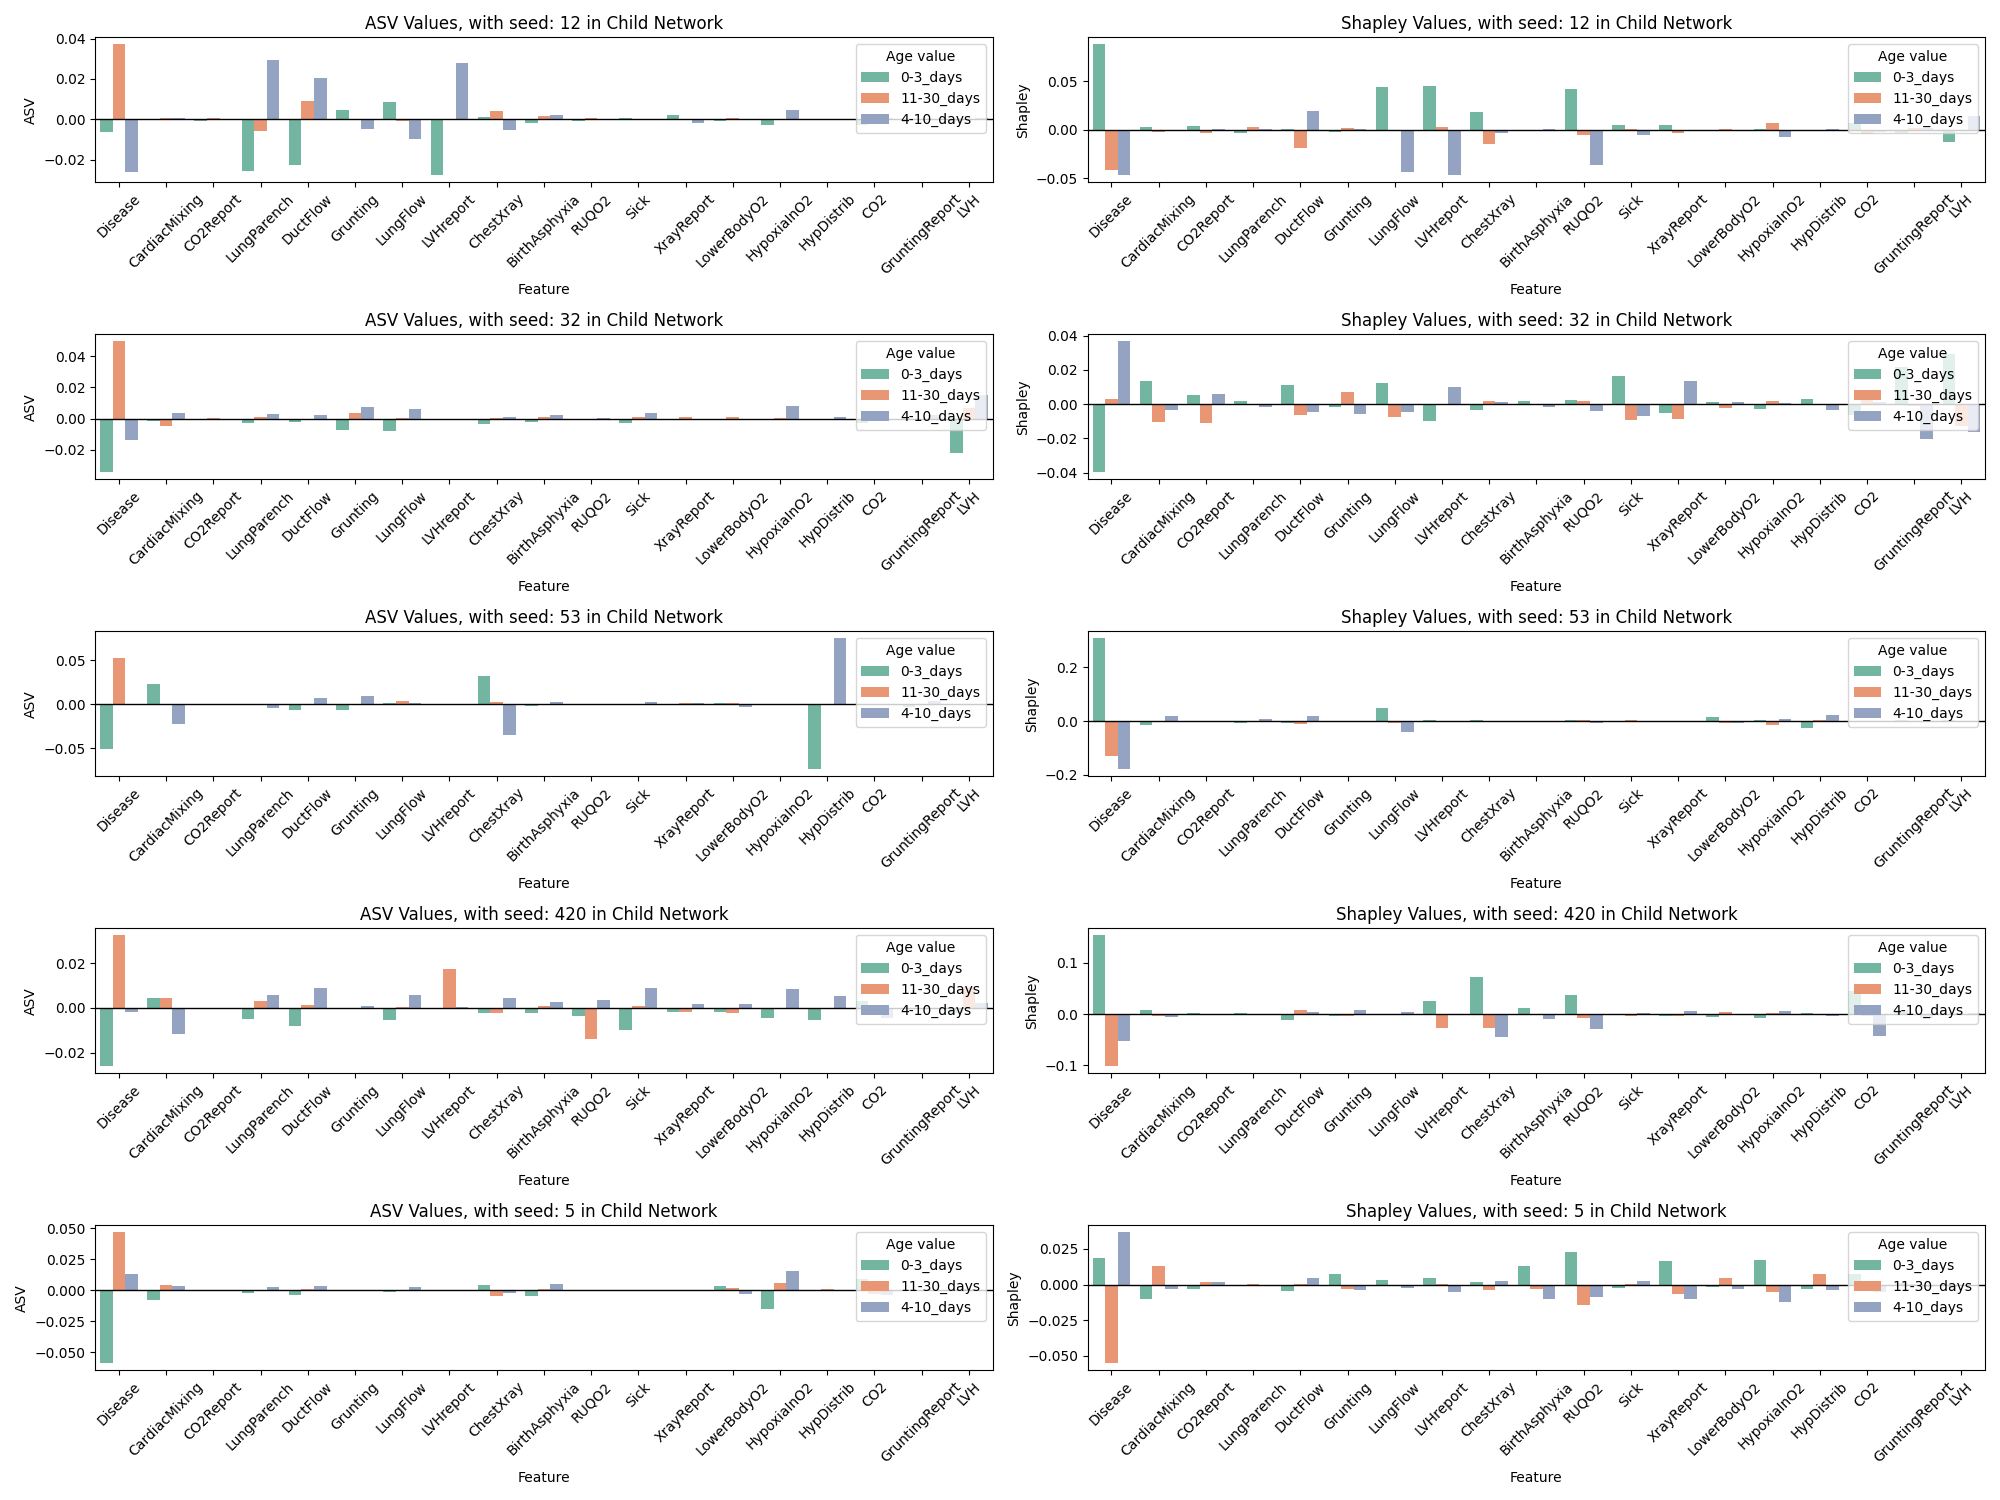
\includegraphics[scale=0.3]{img/asvResults/childMultipleSeedsASVandShapley.png}
    \caption{Comparación de los valores de ASV y Shapley para distintas seeds para la red Child}
    \label{fig:multipleSeedsASVvsShapleyChild}
\end{figure}

\begin{figure}[ht]
    \centering
    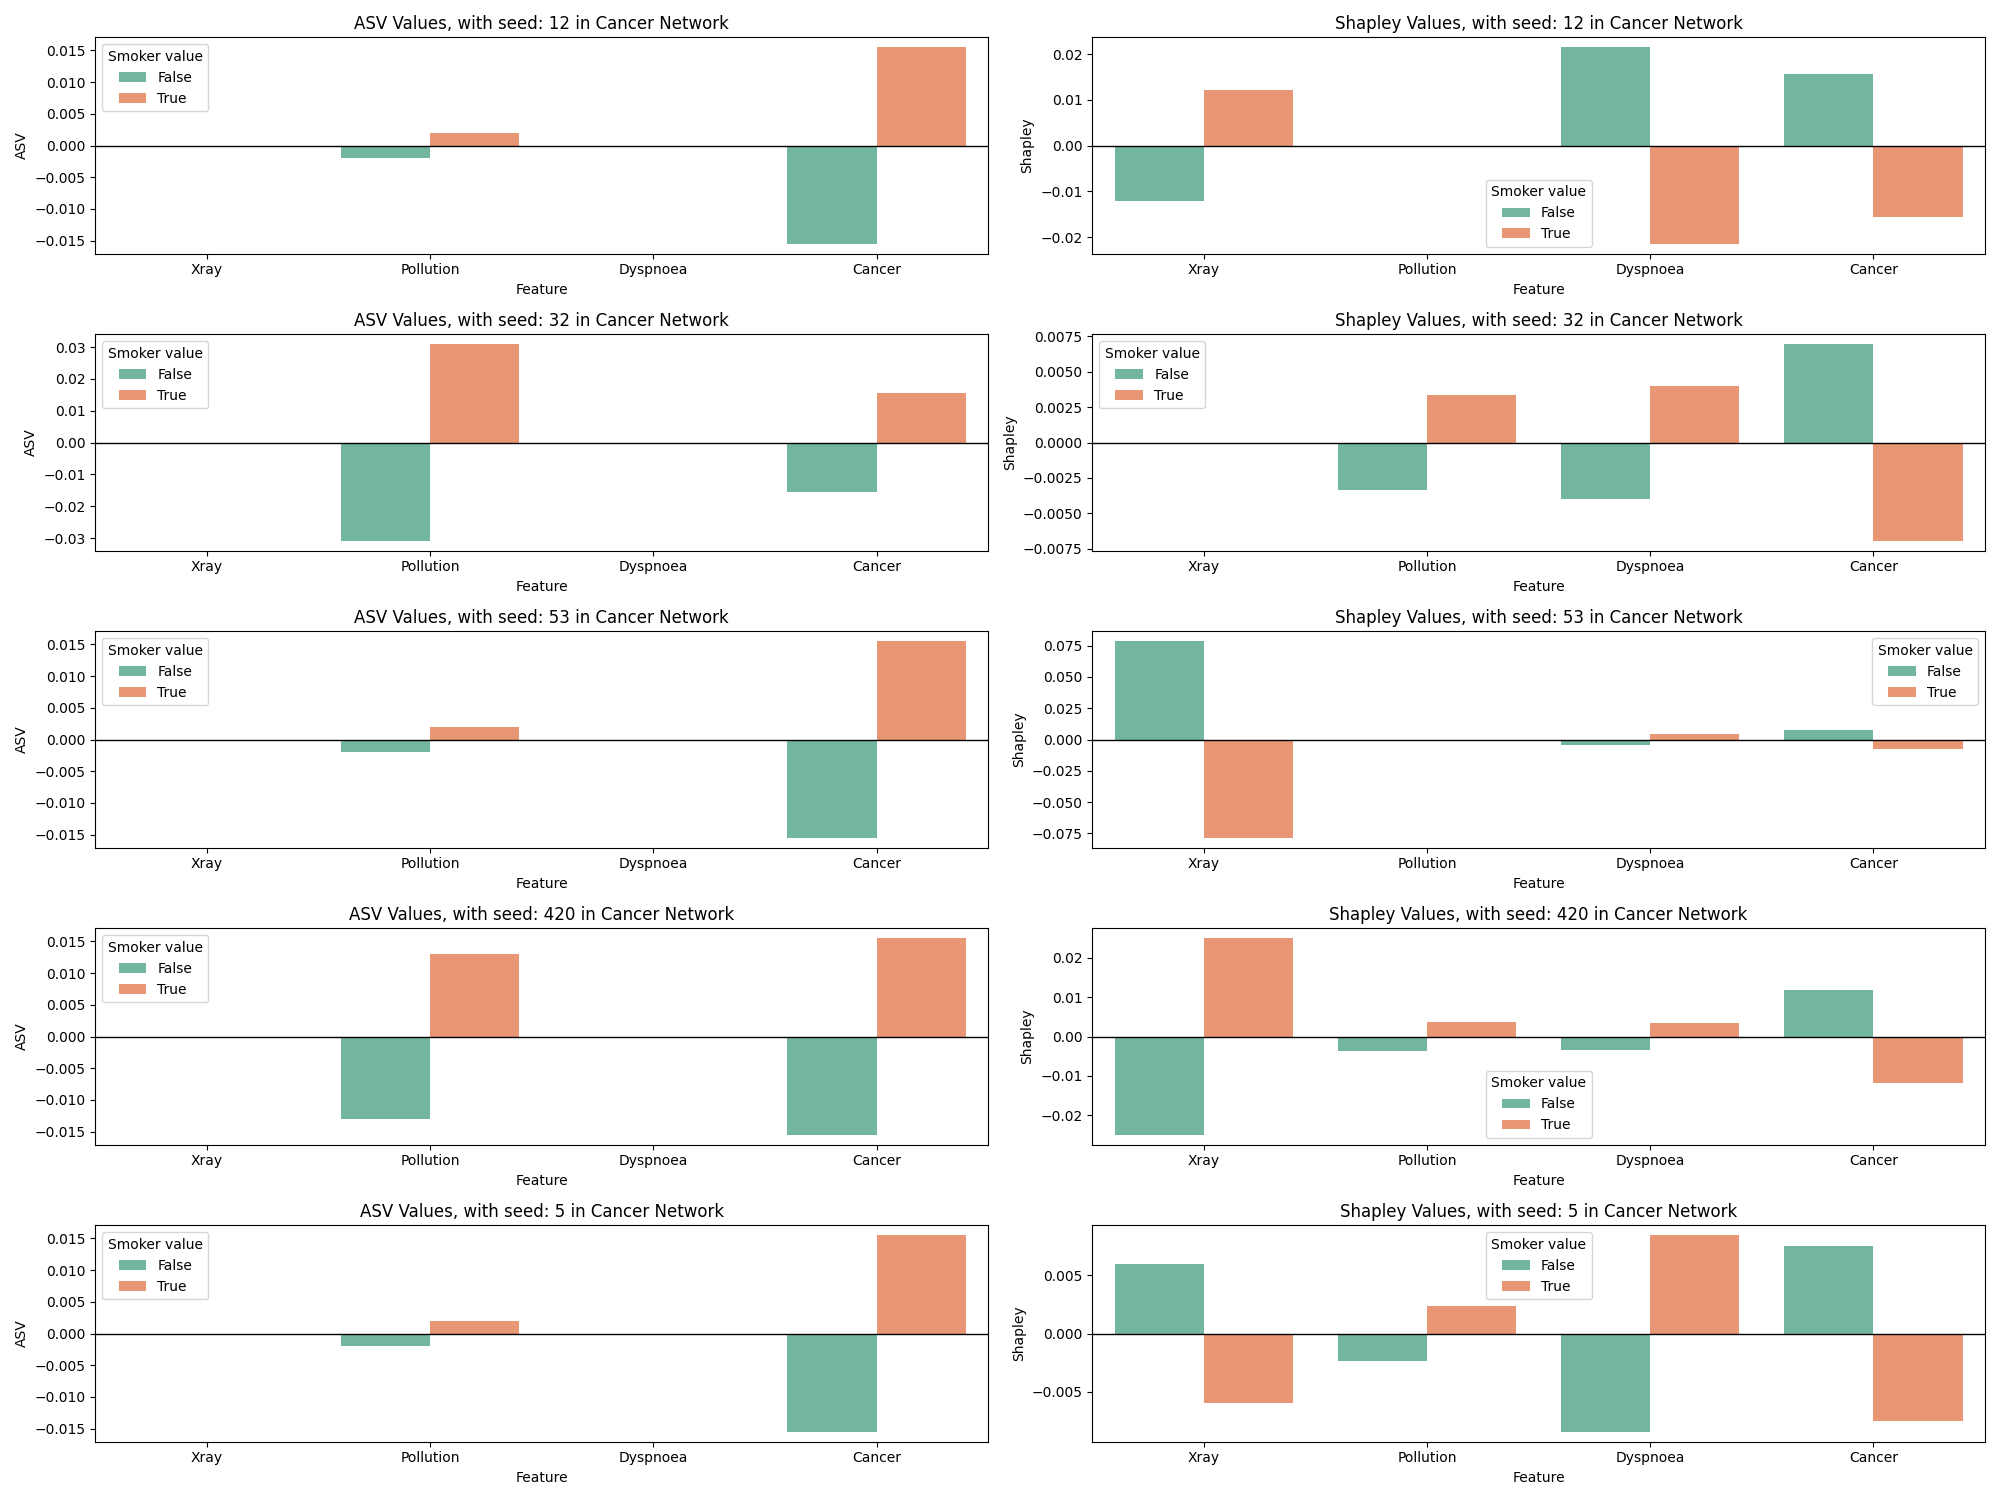
\includegraphics[scale=0.3]{img/asvResults/cancerMultipleSeedsASVandShapley.png}
    \caption{Comparación de los valores de ASV y Shapley para distintas seeds para la red Cancer}
    \label{fig:multipleSeedsASVvsShapleyCancer}
\end{figure}

\end{document}
